\newcommand{\duedate}{17 September 2026}
\documentclass{16384_doc}
\newcommand{\assignmentname}{Assignment 1: Forward Kinematics}

%Feedback url
\newcommand{\feedbackURL}{https://forms.gle/s6zeEiw8dUXC97WYA}

\begin{document}
\maketitle

\tableofcontents

\section{Overview}
Welcome to the first assignment for Robot Kinematics and Dynamics! This assignment aims to build a strong foundation in the core principles of kinematics, including:

\begin{itemize}
\item Degrees of freedom
\item Homogeneous transformations
\item Forward kinematics
\end{itemize}

In the next homework, you will have your first opportunity to interact directly with the robots. 

\subsection{Accessing the Robots}

The robots are accessible in the Robotics Engineering Lab (REL) and will be available for use starting next week. Please be mindful of others and share the robotic resources fairly. We ask that you keep your sessions with the robots to a maximum of 30 minutes at a time to ensure that all students have equal opportunity to engage with the technology. An online google sheet that acts as a scheduler will become available online in the future.

\section{Background}

This section outlines the essential concepts that will be covered in this assignment. You are expected to be familiar with these terms as they are fundamental to understanding robot kinematics and dynamics. Reference the attached summary of the relevant topics annexed in this document. 

\subsection{Key Concepts}

\begin{itemize}
    \item \textbf{Coordinate Frames}:
    Understand the use of coordinate frames in robotics, including origin points and orthonormal axes. All frames used will be right-handed.
    
    \item \textbf{Point and Vector}:
    Learn the representation of points and vectors within different coordinate frames. Points denote fixed positions in space, while vectors represent quantities like displacements and forces that have both magnitude and direction.
    
    \item \textbf{Rigid Body and Rigid Motion}:
    Explore the properties of rigid bodies, which maintain constant distances between points, and understand rigid motions like translations and rotations that can be applied to these bodies.
    
    \item \textbf{Mathematical Spaces}:
    Familiarize yourself with $\mathbb{R}^2$ for two-dimensional Cartesian space and $SE(2)$ for the combination of positional and rotational parameters in two dimensions.
    
    \item \textbf{Workspace}:
    Analyze the workspace of a robot, which is the set of all points that the robot’s end effector can reach through any configuration of its joints.
\end{itemize}

\subsection{Robots and Robot Diagrams}

Gain a clear understanding of the structural and operational aspects of robots used in this class, focusing on:

\begin{itemize}
    \item \textbf{Links and Joints}: Links are the rigid bodies making up the robot, and joints are the connections allowing constrained relative motions between these links.
    
    \item \textbf{Revolute and Prismatic Joints}: Understand the two main types of joints used in the class, where revolute joints allow rotational movement and prismatic joints permit translational movement along an axis.
    
    \item \textbf{Kinematic Chain}: Comprehend the configuration of a robot as a series of links connected by joints, forming a chain that determines the robot’s motion capabilities.
    
    \item \textbf{Degrees of Freedom}: Determine the degrees of freedom in a system, which represent the number of independent movements allowed in the system.
\end{itemize}

\subsection{Transforms in Robotics}

\begin{itemize}
    \item \textbf{Rigid Motions and Transforms in Two Dimensions}: Delve into how rotations and translations are used to describe the motion of points and the transformation between coordinate frames.
\end{itemize}

\subsection{Learning Objectives}

Through this assignment, you are expected to:

\begin{itemize}
    \item Apply the concepts of coordinate frames to define the motion and orientation of robot components.
    \item Use transformations to calculate the positions of points and orientations of links in various robot configurations.
    \item Understand the physical limitations and capabilities of robots through the analysis of workspaces and degrees of freedom.
\end{itemize}

\subsection{Course Logistics}

In this class you would be using the following websites regularly:

% \begin{itemize}
    % \item \href{https://google.com}{Piazza}: This is the best way to ask course staff questions, and see course announcements.
    % \item \href{http://gradescope.com}{Gradescope}: Create an account using your CMU email. You should have already been added to the course. If you haven't, please contact the course staff via email or Piazza post.
% \end{itemize}
\begin{itemize}
    \item \href{https://canvas.cmu.edu/courses/56566}{Canvas}: The main course web page. This links to everything relevant to the class (including the next two links).
    \item \href{https://canvas.cmu.edu/courses/56566/external_tools/11046}{Piazza}: This is the best way to ask course staff questions, and see course announcements.
    \item \href{https://canvas.cmu.edu/courses/56566/external_tools/11047?display=borderless}{Gradescope}: This is where you will be turning in your homework. You should have already been added to the course. If you haven't, please contact the course staff via email or Piazza post.
\end{itemize}

\newpage
\writtenSection
\newpage

\section{Theory Questions}
\begin{questions}

    \titledquestion{\textbf{Matrix Analysis Review}}[5]
    Given the Matrix
    $ A = \begin{bmatrix}
    -\sin(\theta_1) - \sin(\theta_1 + \theta_2) & -\sin(\theta_1 + \theta_2) \\
    \phantom{-}\cos(\theta_1) + \cos(\theta_1 + \theta_2) & \phantom{-}\cos(\theta_1 + \theta_2)
\end{bmatrix} $

    \begin{enumerate}[label=\alph*.]
        \item \text{[1 point]} Is A an element of $SO(2)$?
        \item \text{[1 point]} For what values of $\theta_2$ does $\rank(A) = 1$? Are there similar values for $\theta_1$?
        \item \text{[1 point]} What is the inverse of $A$?
        \item \text{[1 point]} Using (2), what values of $\{\theta_1, \theta_2\}$ can you \emph{not} solve $Ax = b$, where $x$ and $b$ are column vectors?
        \item \text{[1 point]} Algebraically write the constraint that defines the set of vectors $b$ that have a solution when $\rank(A)=1$.
    \end{enumerate}

    \begin{tcolorbox}[height=15cm]
        % TODO: ENTER YOUR ANSWER HERE
    \end{tcolorbox}

\titledquestion{\textbf{Basic Transformations}}[5]
    %Let \vec{t} = \smcolvec{-1\\1}, \th~=-\piover{4}
    Let $t = \begin{bmatrix} -1 \\ 1 \end{bmatrix}, \theta = \frac{\pi}4$

    \begin{enumerate}[label=\alph*.]
        \item \text{[1 point]} Write the matrix $H_1$ that is the homogeneous transformation that translates a
        point by $t$.
        \item \text{[1 point]} Write the matrix $H_2$ that is the homogeneous transformation that rotates a
        point by $\theta$.  
        \item \text{[2 points]} Show \emph{algebraically} that $H_1 H_2$ is not equal to $H_2 H_1$. 
        \item \text{[1 point]} Show \emph{geometrically} (either via transforming a body defined by set coordinates mathematically or via drawing the transformation) that $H_1 H_2$ is not equal to $H_2 H_1$.
    \end{enumerate}
        


    \begin{tcolorbox}[height=16cm]
        % TODO: ENTER YOUR ANSWER HERE
    \end{tcolorbox}
    
\titledquestion{\textbf{Basic degrees of Freedom}}[5]
    How many degrees of freedom do each of these robots have (assume $\mathbb{R}^2$)? Show your work with the Grubler formula for part 4. 
    

    \begin{enumerate} [label=\alph*.]
        \item \text{[1 point]}
        \begin{align*}
        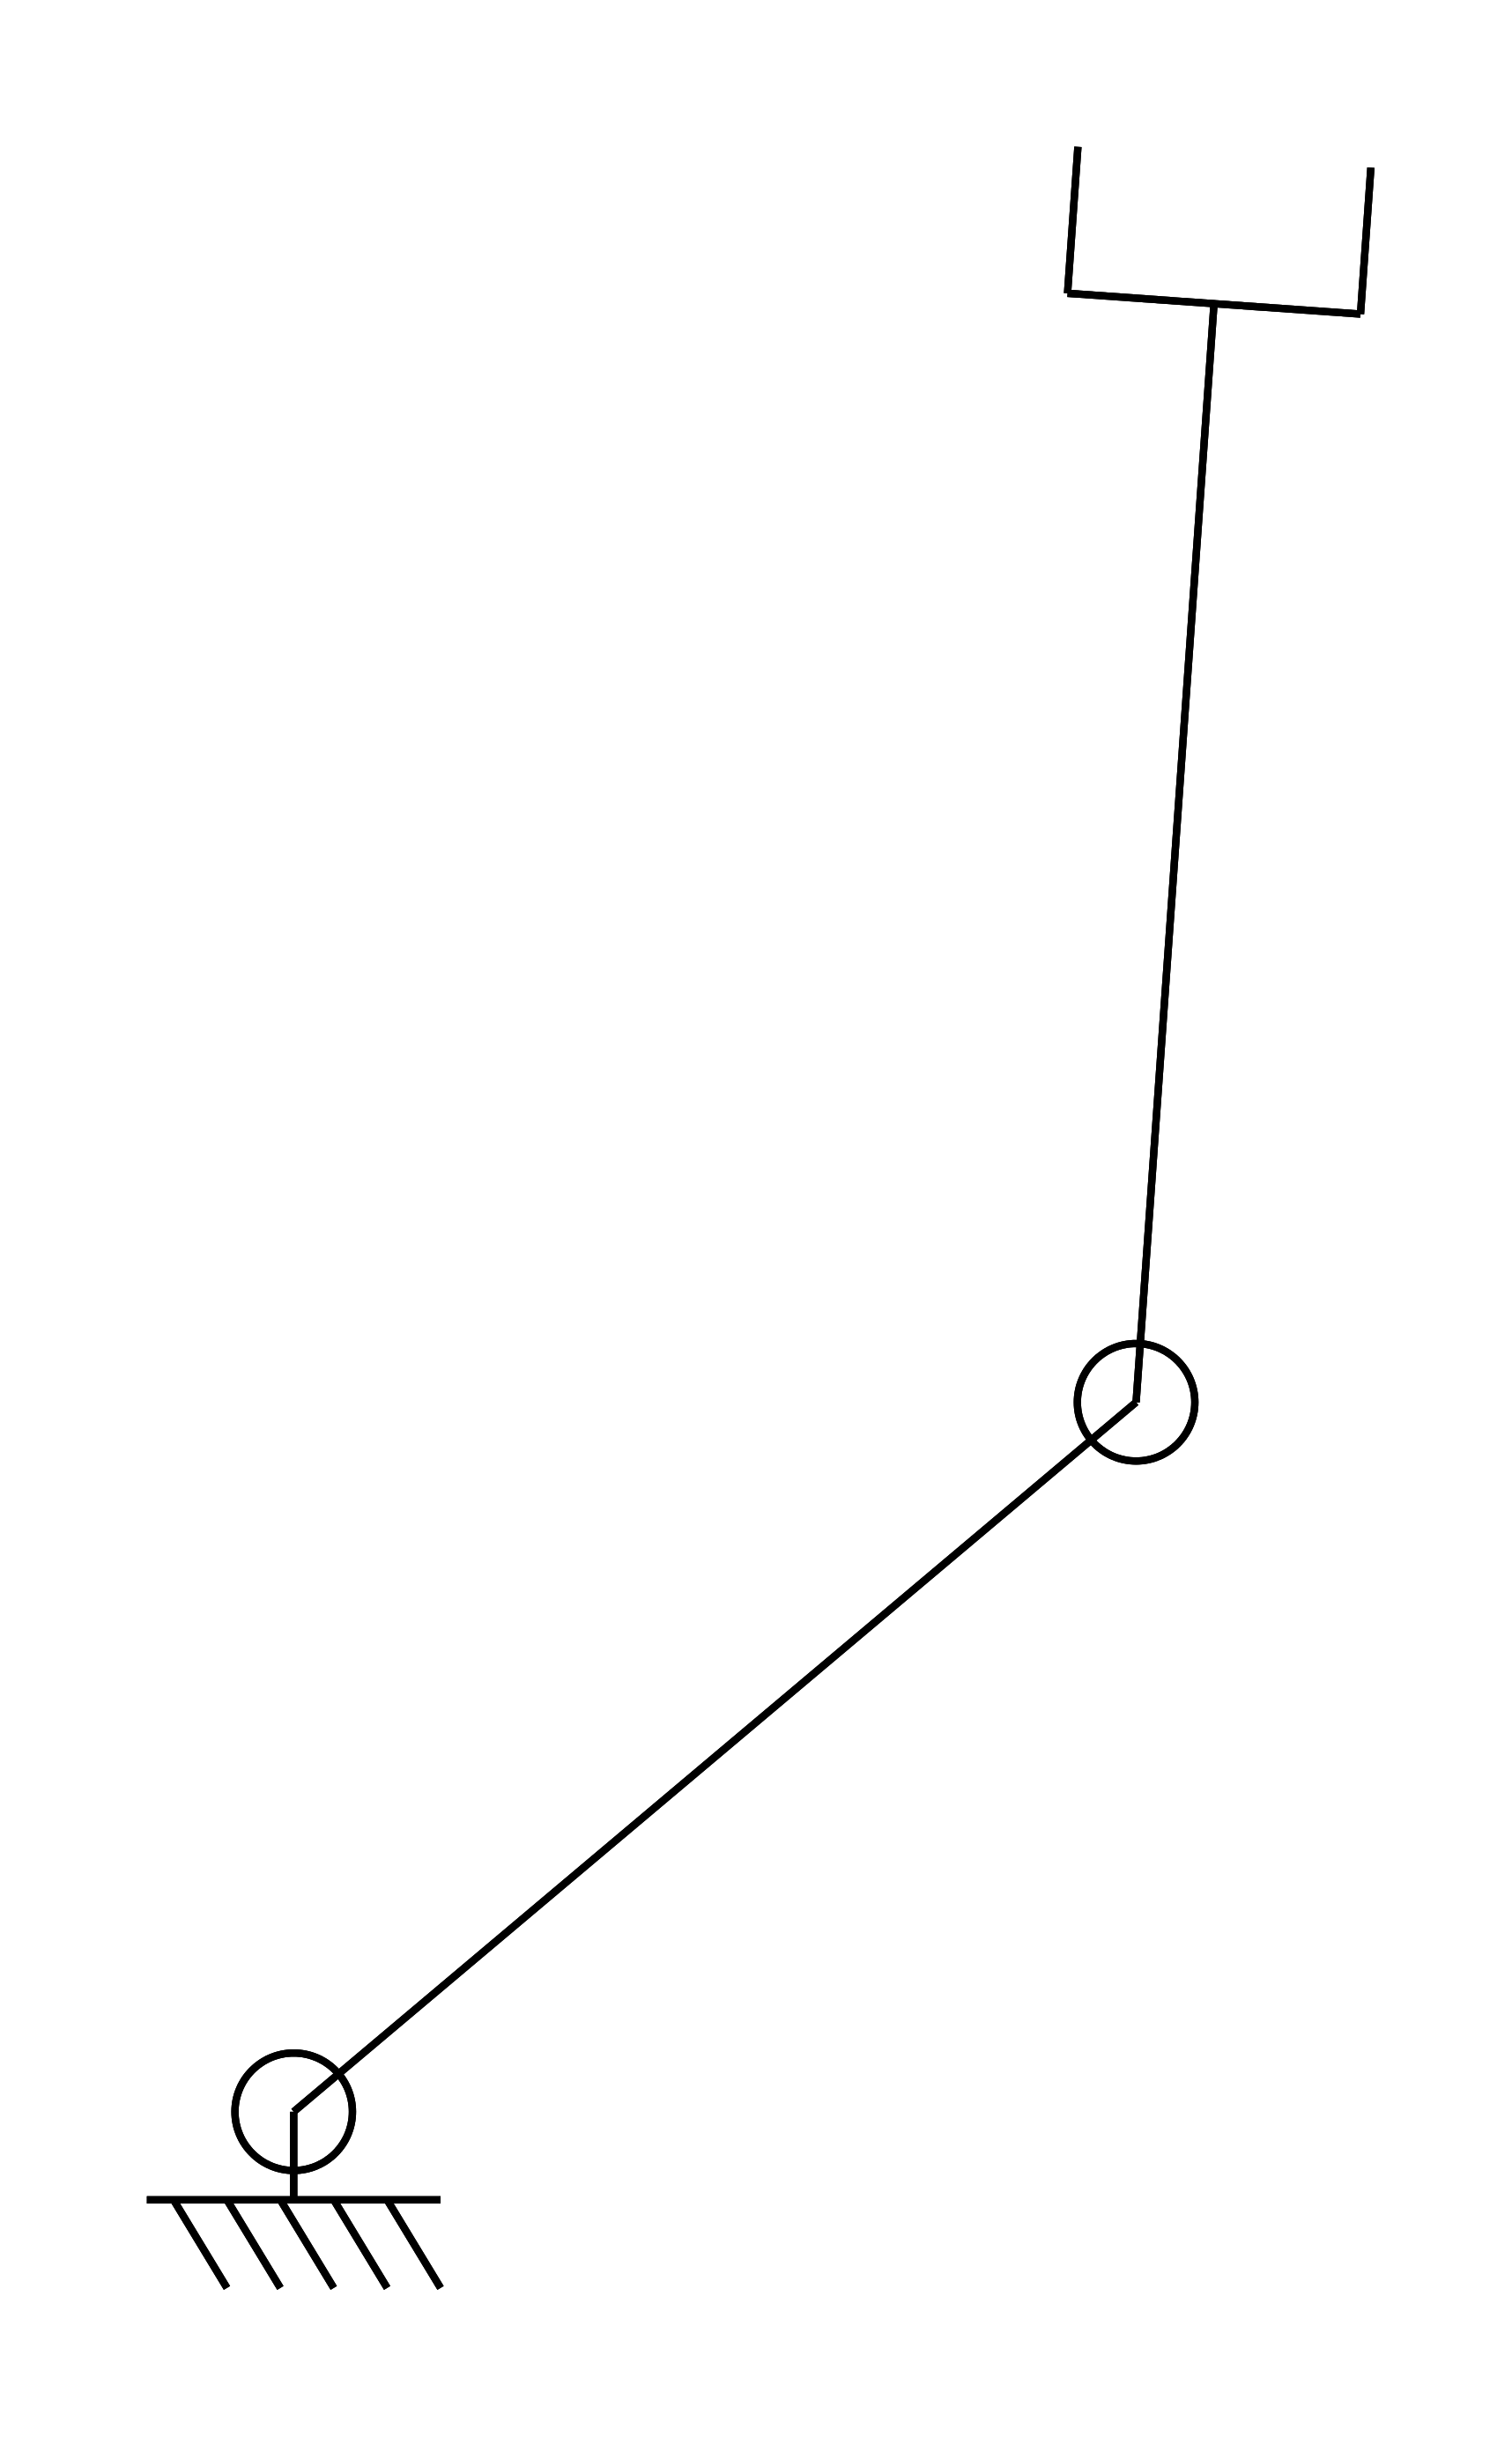
\includegraphics[scale=0.07]{generated_figures/robot_1a.png}
        \end{align*}

        \begin{tcolorbox}[height=3cm]
         % TODO: ENTER YOUR ANSWER HERE
        \end{tcolorbox}

        \item \text{[1 point]}
        \begin{align*}
        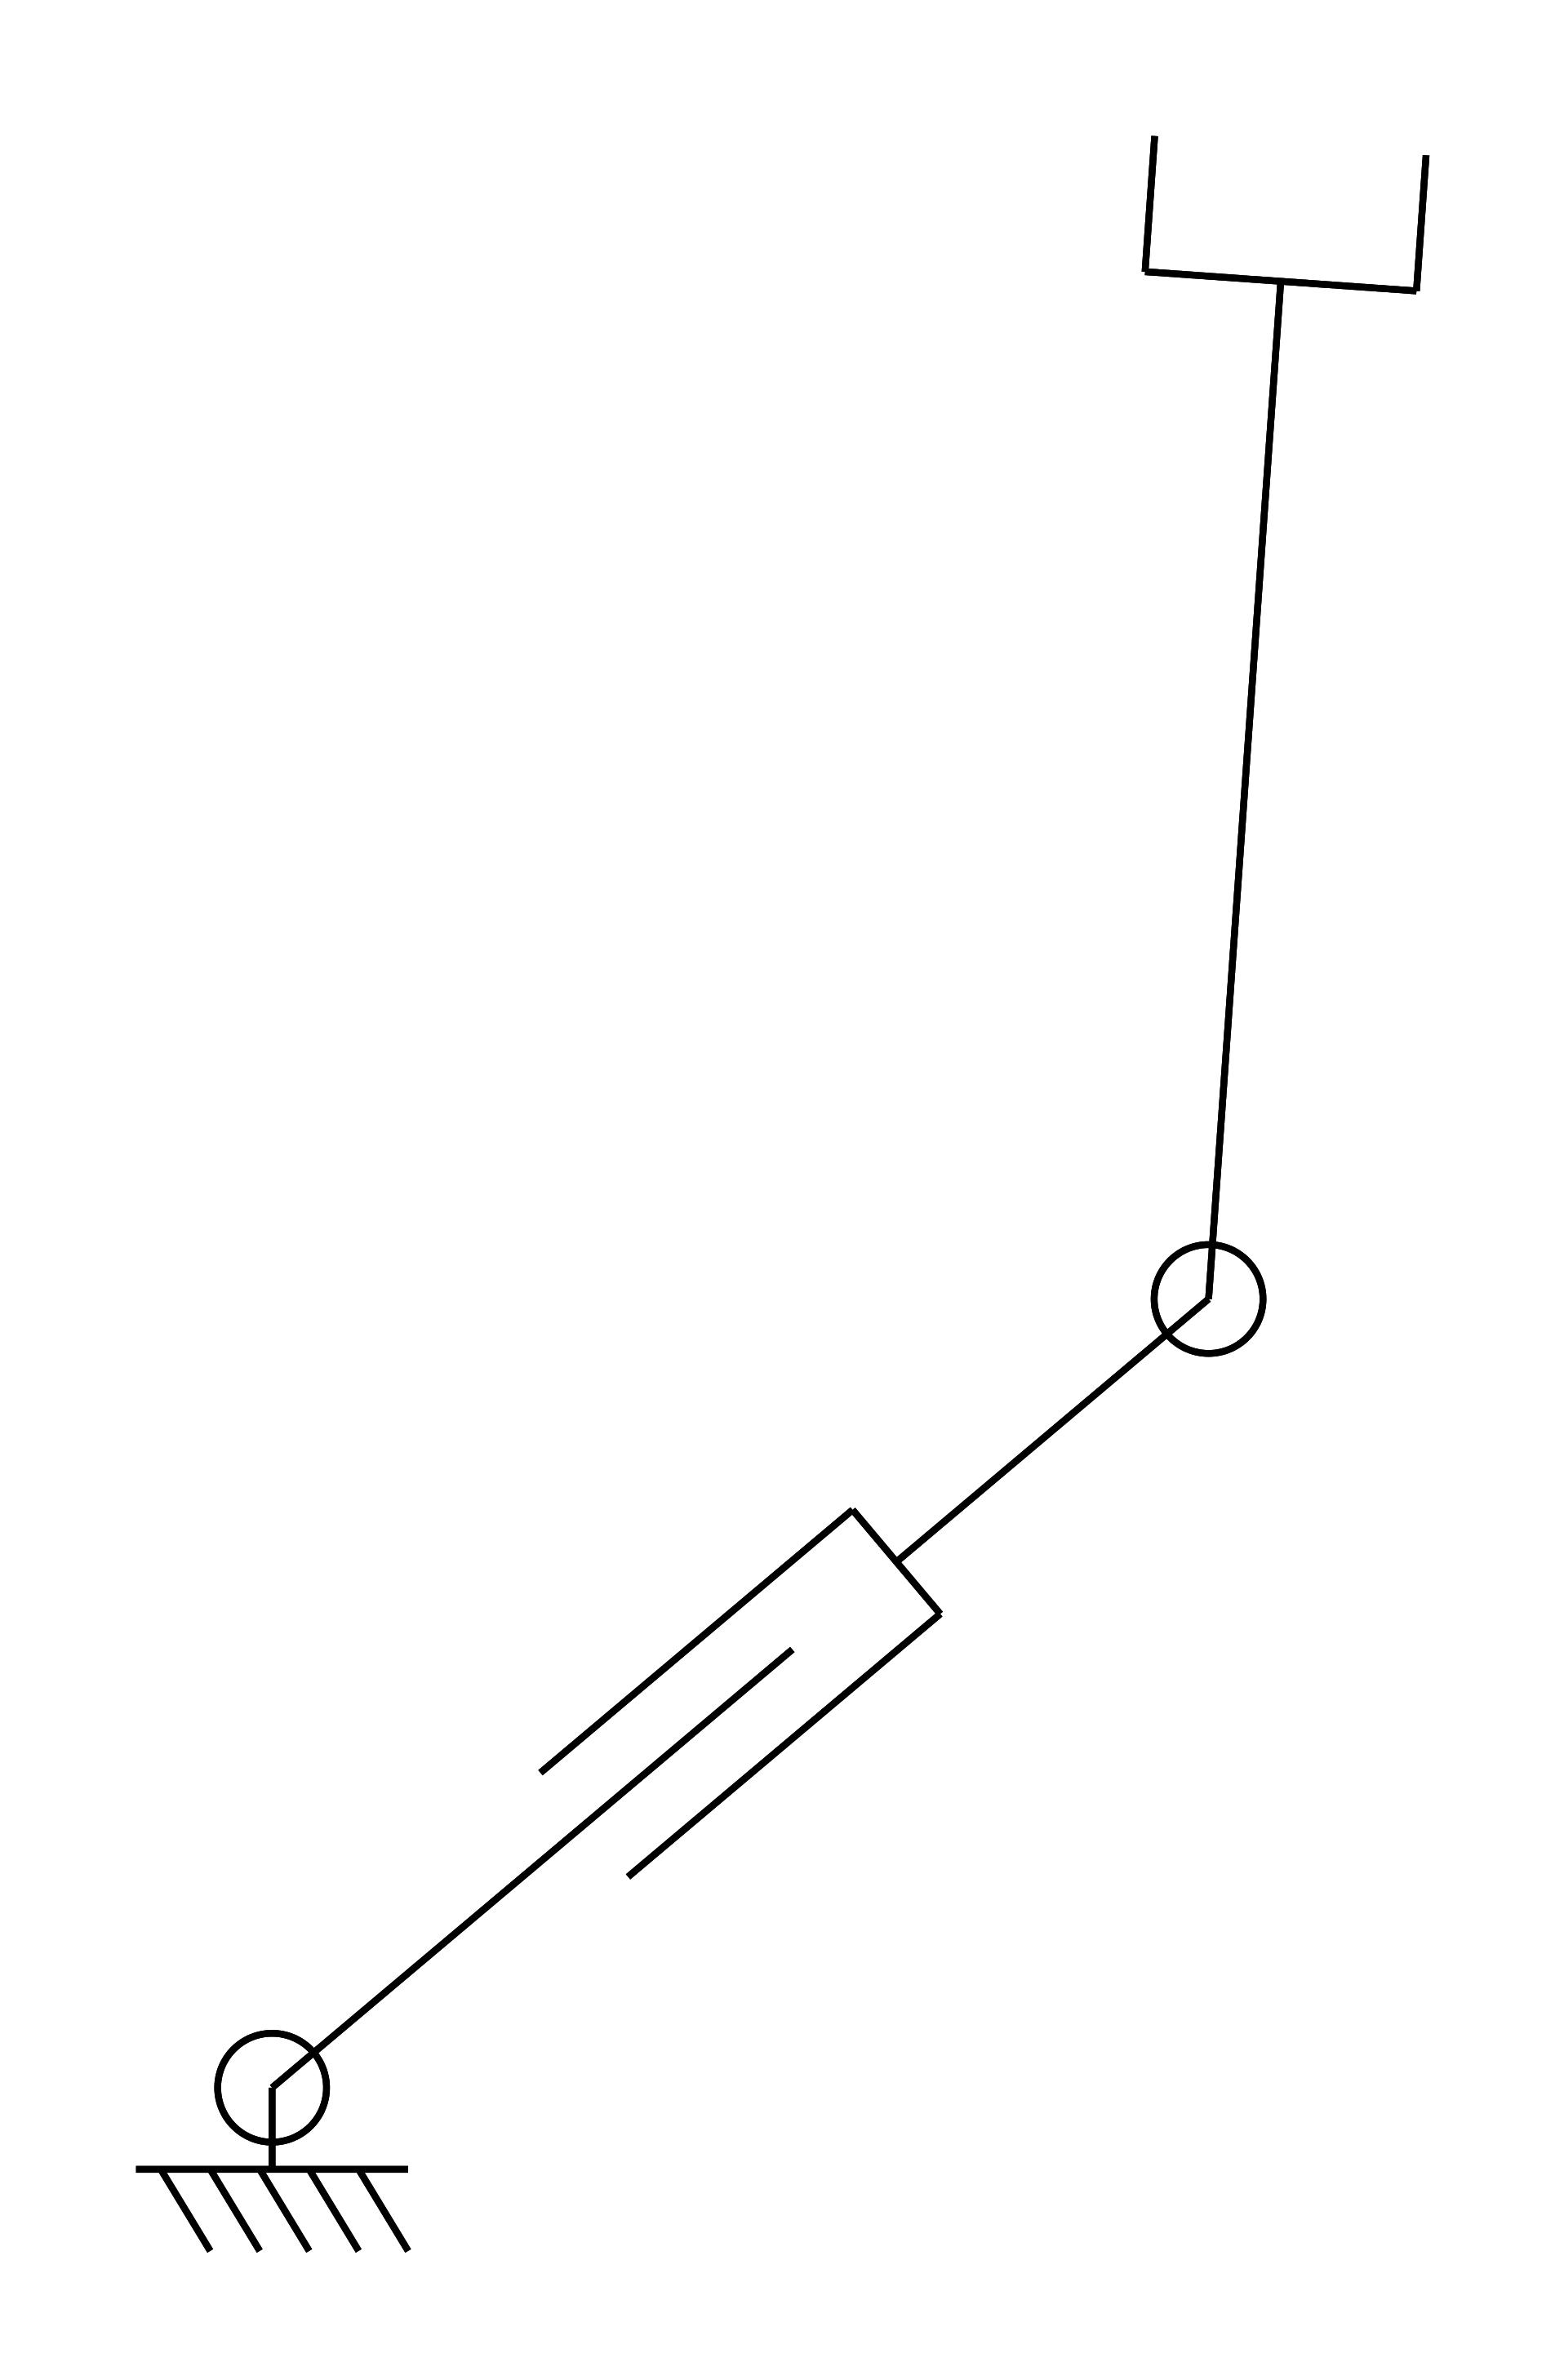
\includegraphics[scale=0.07]{generated_figures/robot_1b.png}
        \end{align*}
        
        \begin{tcolorbox}[height=3cm]
         % TODO: ENTER YOUR ANSWER HERE
        \end{tcolorbox}


        \item \text{[1 point]}
        \begin{align*}
        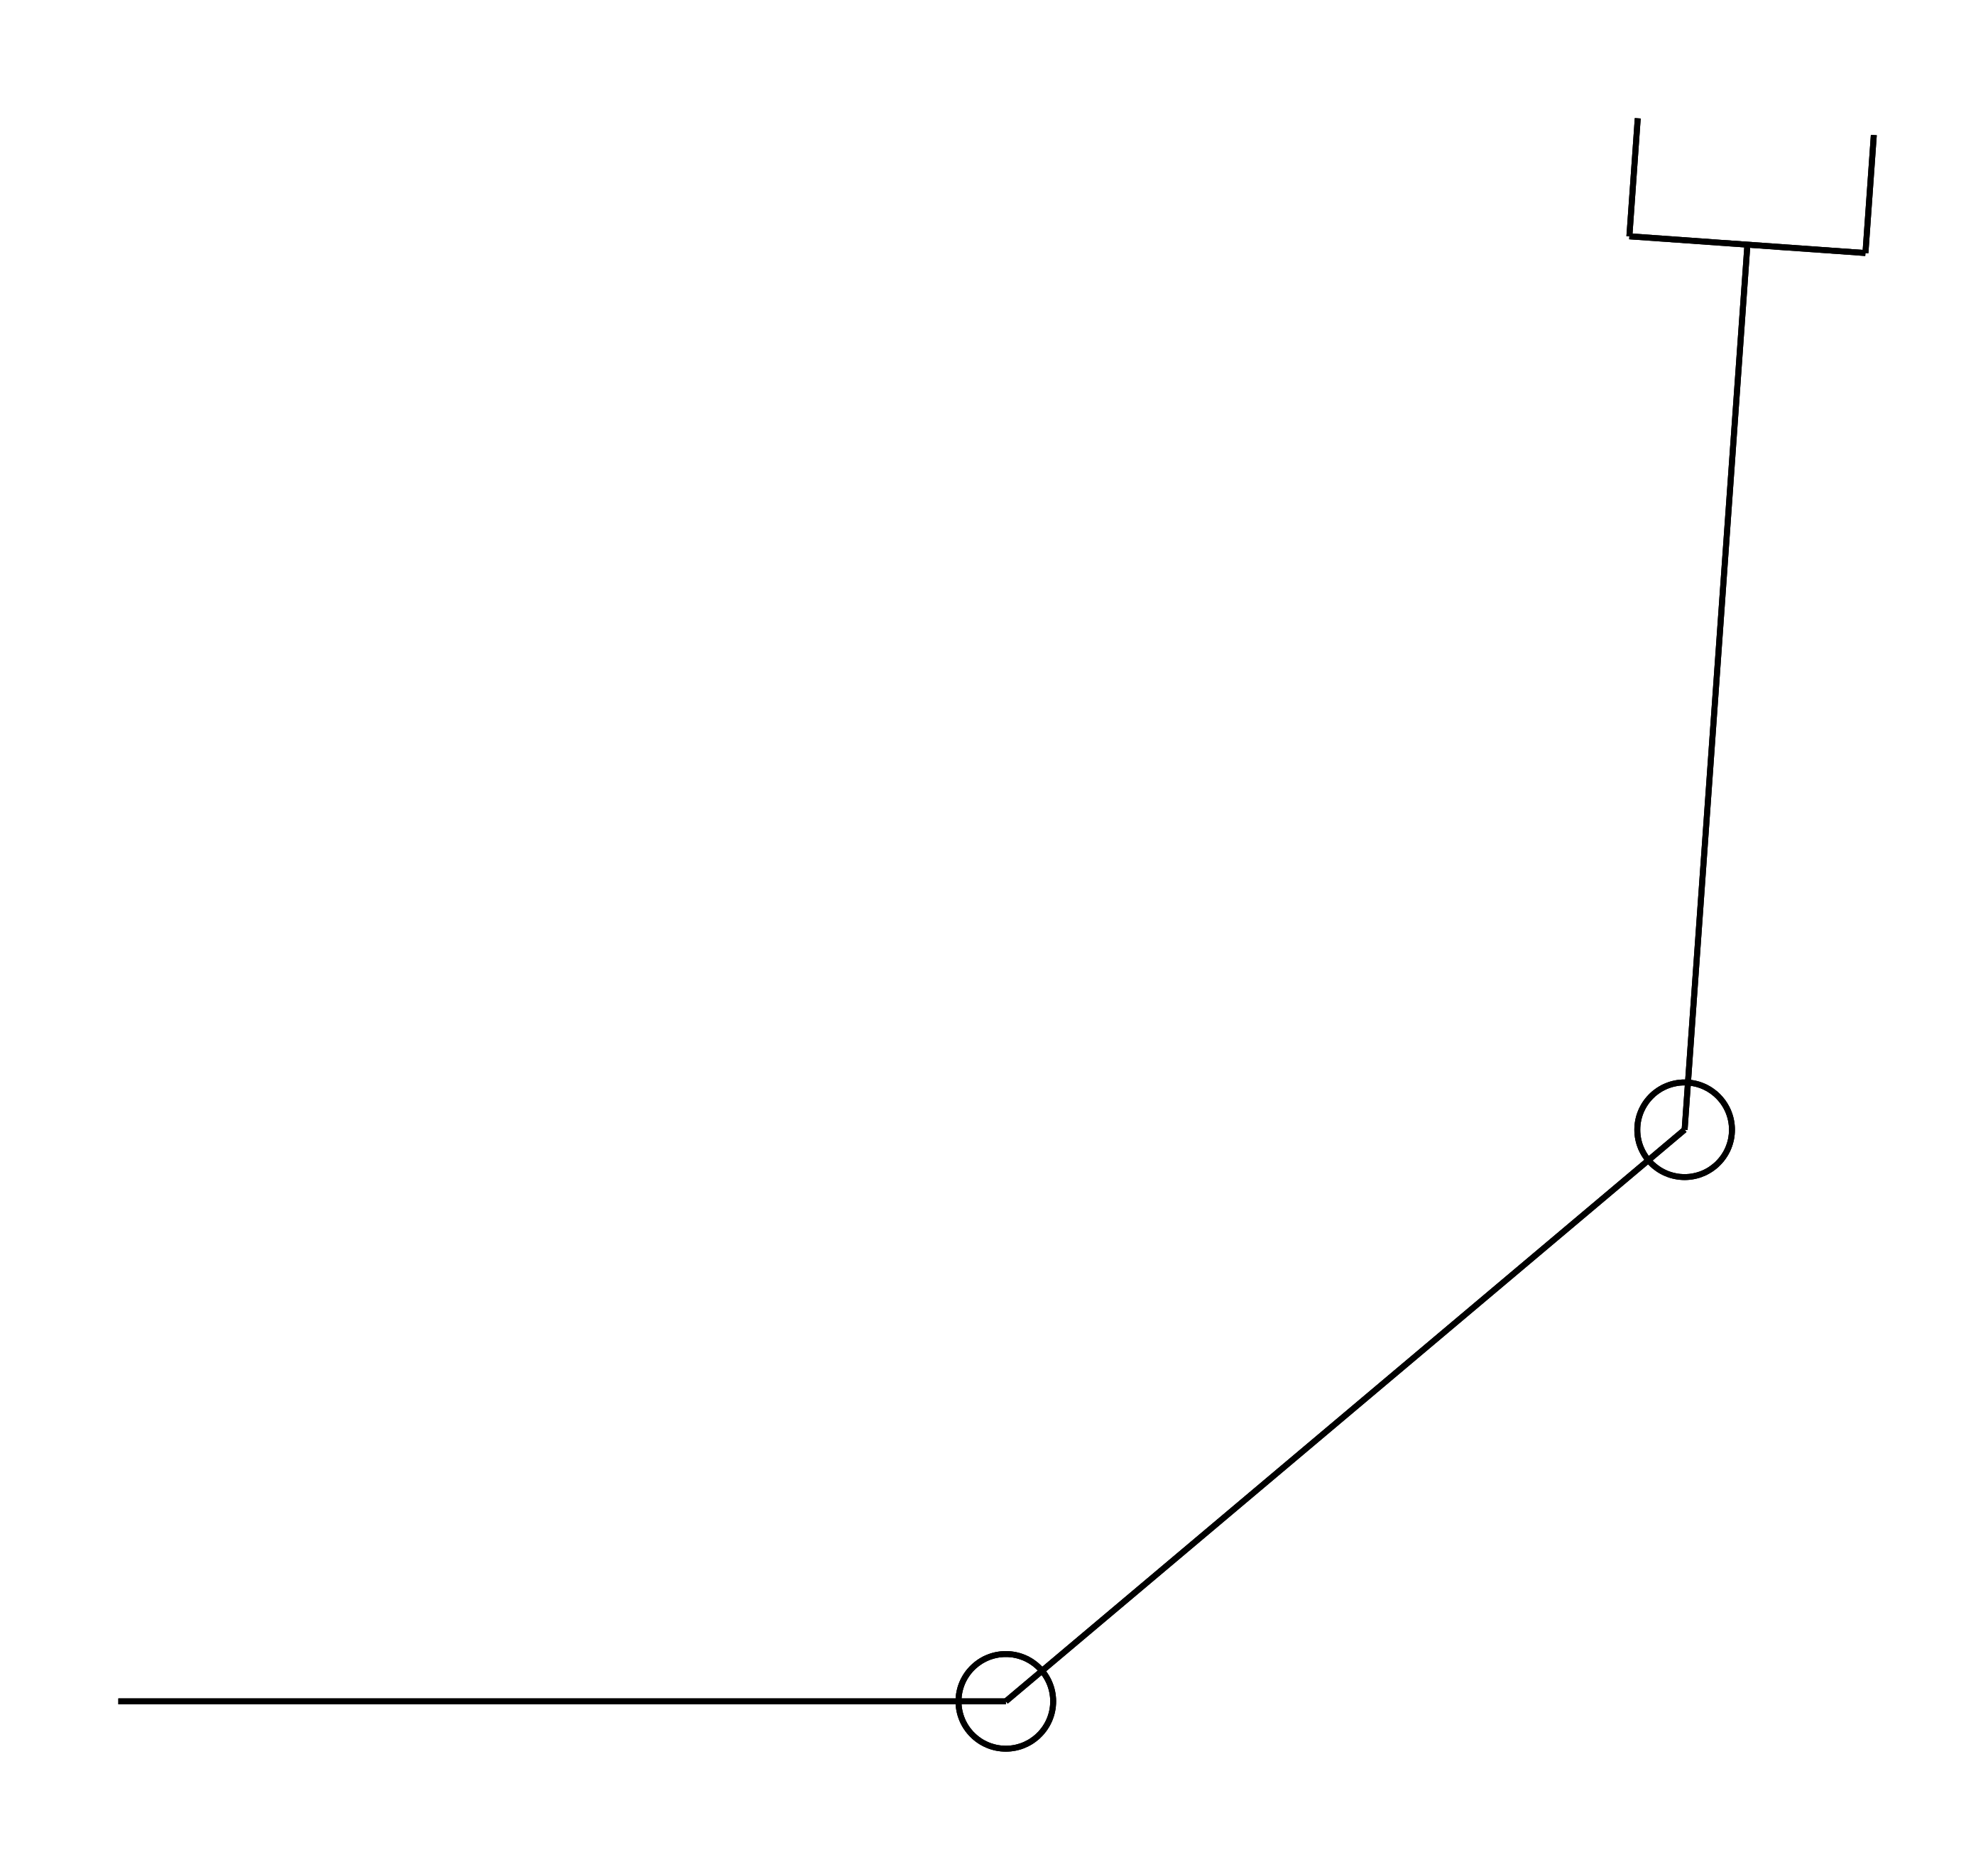
\includegraphics[scale=0.07]{generated_figures/robot_1c.png}
        \end{align*}
        
        \begin{tcolorbox}[height=3cm]
         % TODO: ENTER YOUR ANSWER HERE
        \end{tcolorbox}
        
        \item \text{[2 point]}
        \begin{align*}
        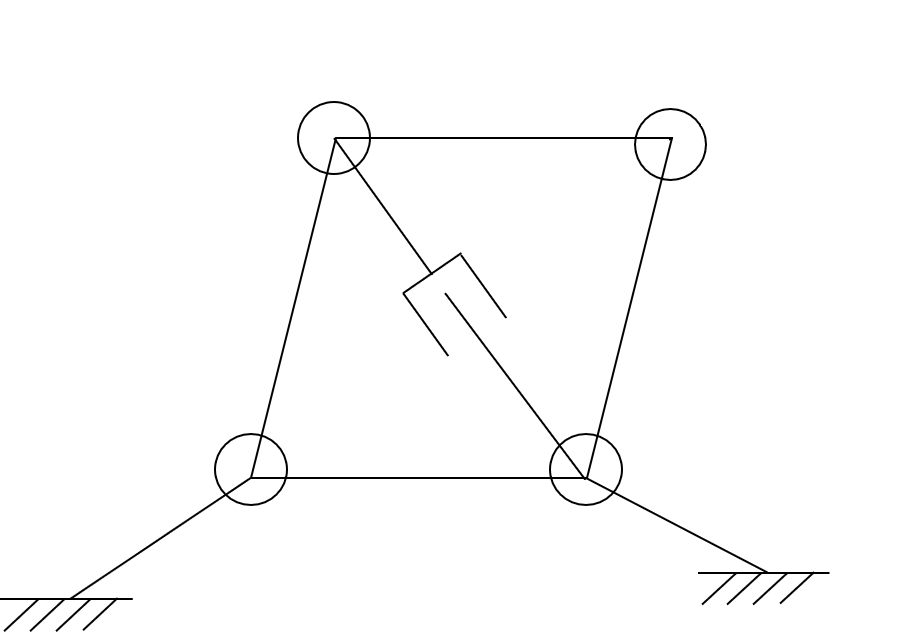
\includegraphics[scale=1]{generated_figures/robot_1d.png}
        \end{align*}
        
        \begin{tcolorbox}[height=10cm]
         % TODO: ENTER YOUR ANSWER HERE
        \end{tcolorbox}
        
    %\end{parts}
    \end{enumerate}

\titledquestion{\textbf{Real-world DOF Determination}}[20]

This exercise involves analyzing the degrees of freedom in human arms and their interaction with external systems like vehicles or rehabilitation robots. Understanding these concepts is critical in fields such as biomechanics, robotics, and ergonomic design.


\begin{enumerate}[label=\alph*.]
    \item \textbf{[5 points] Degrees of Freedom in the Human Arm:}
    Determine the number of degrees of freedom starting from your shoulder and going to your palm (excluding fingers and thumb). List the degrees of freedom at the shoulder, elbow, forearm, and wrist, then add them up.


    \begin{tcolorbox}[height=3cm]
         % TODO: ENTER YOUR ANSWER HERE
    \end{tcolorbox}

    \item \textbf{Degrees of Freedom While Driving:}
    Assuming your arms have $n$ degrees of freedom, analyze the combined system of your arms and the steering wheel while driving. Consider that your torso is stationary due to a seatbelt, and your 2 hands are fixed on the steering wheel at specific positions and angles. 

    \begin{enumerate} [label=(\roman*)]
        \item \text{[2 points]} In 3 dimensional space $SE(3)$, 6 constraints are placed on an arm by requiring its end effector be at a certain position and angle. Calculate and explain the total degrees of freedom available in terms of $n$ in the 2-arms-plus-steering wheel system, \textbf{if the steering wheel cannot rotate or move}.
        \begin{tcolorbox}[height=3cm]
         % TODO: ENTER YOUR ANSWER HERE
        \end{tcolorbox}

        \item \text{[1 points]} How many degrees of freedom does a steering wheel have when not frozen at a specific angle (i.e. it can rotate as a standard steering wheel)? 
        \begin{tcolorbox}[height=3cm]
         % TODO: ENTER YOUR ANSWER HERE
        \end{tcolorbox}

        \item \text{[2 points]} Suppose the steering wheel is now unfixed (i.e. it can rotate like a standard steering wheel) just like in the previous problem.  Calculate and explain the total degrees of freedom available in terms of $n$ in the 2-arms-plus-steering wheel system.
        \begin{tcolorbox}[height=3cm]
         % TODO: ENTER YOUR ANSWER HERE
        \end{tcolorbox}
    \end{enumerate}

    \item \textbf{[10 Points] Human-Robot Interaction in Rehabilitation:}
    Referring to the figure below of a robot used for human arm rehabilitation. Determine the number of degrees of freedom in the chain formed by the human arm coupled with the rehabilitation robot. \textbf{Note: Assume the human torso represented by the stick figure is frozen and part of the ground for the purposes of DOF calculation).}
    \begin{align*}
        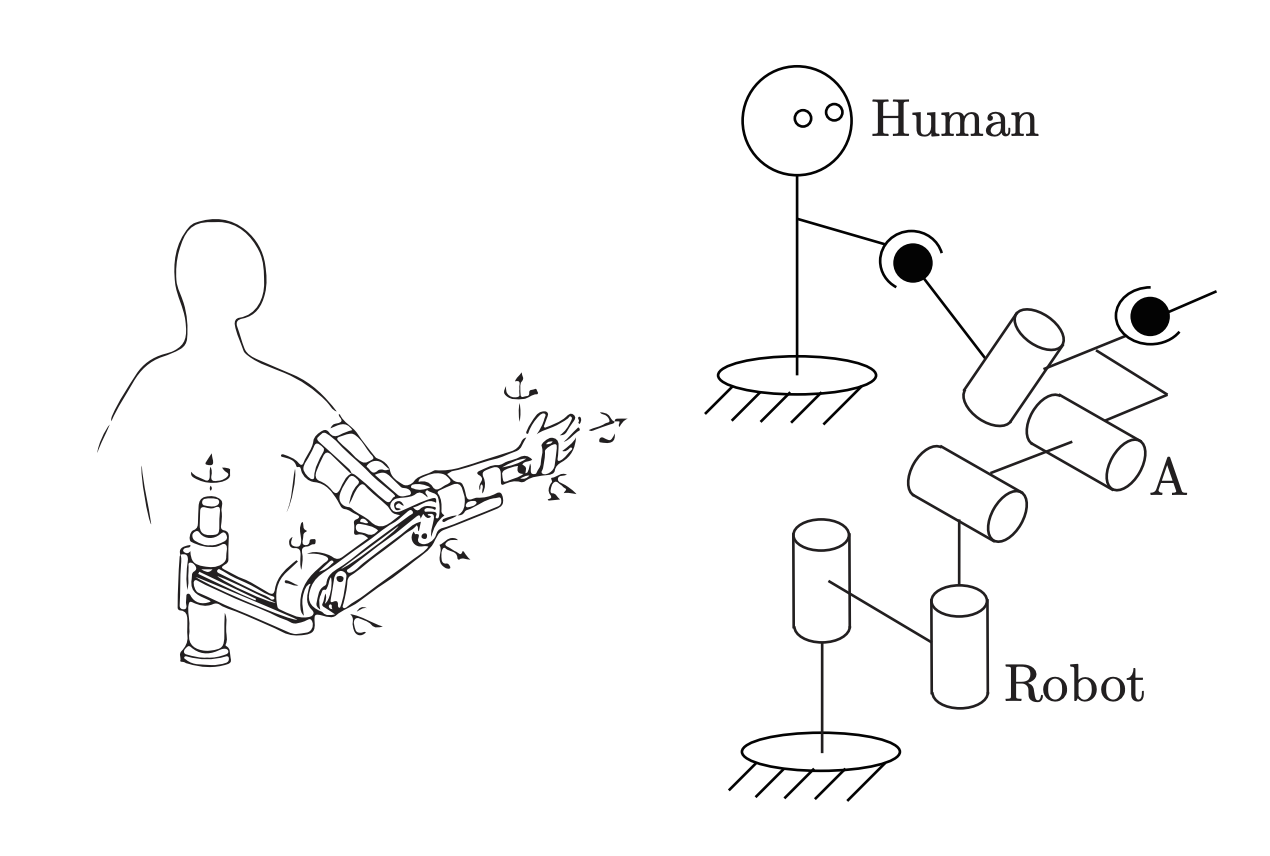
\includegraphics[scale=0.4]{generated_figures/q4_3.png}
    \end{align*}
    \begin{enumerate} [label=(\roman*)]
        \item \text{[5 points]} List the number of links, and the number of each type of joint in the diagram.
        \begin{tcolorbox}[height=3cm]
         % TODO: ENTER YOUR ANSWER HERE
        \end{tcolorbox}

        \item \text{[5 points]} Calculate the number of degrees of freedom. 
        \begin{tcolorbox}[height=3cm]
         % TODO: ENTER YOUR ANSWER HERE
        \end{tcolorbox}

    \end{enumerate}
\end{enumerate}

    \titledquestion{\textbf{Rotation Matrices}}[3]
    %Let \vec{p} = \smcolvec{10\\0}.
    Let $p = \begin{bmatrix} 10 \\ 0 \end{bmatrix}$
    
    %\begin{parts}
    \begin{enumerate}[label=\alph*.]
    %\part[1] 
    \item \text{[1 point]}
    Let $R$ be the rotation matrix representing a rotation by $\frac{\pi}4$.  Find $R$.
    \begin{tcolorbox}[height=3cm]
         % TODO: ENTER YOUR ANSWER HERE
    \end{tcolorbox}
    %\part[1] 
    \item \text{[1 point]}
    Let $p'$ be the result of applying $R$ to $p$.  Find $p'$.

    \begin{tcolorbox}[height=3cm]
         % TODO: ENTER YOUR ANSWER HERE
    \end{tcolorbox}
    %\part[1] 
    \item \text{[1 point]}
    Draw and label a set of axes, and plot $p$, and $p'$ in this frame.

    \begin{tcolorbox}[height=3cm]
         % TODO: ENTER YOUR ANSWER HERE
    \end{tcolorbox}
    \end{enumerate}

    

    %\newpage

    \titledquestion{\textbf{[5 points] Inverting Homogeneous Transformations}}[5]
    % Algebraically show that if \H{i}{j} =
    % \smcolvec{\R{i}{j}&\t{i}{j}\\\trans{\vec{0}}&1}, then \inv{\H{i}{j}} =
    % \smcolvec{\trans{\R{i}{j}}&-\trans{\R{i}{j}}\t{i}{j}\\\trans{\vec{0}}&1}.
    
    Given $H_i^j = \begin{bmatrix} R_i^j & d_i^j \\ \mathbf{0} & 1 \end{bmatrix}$, \emph{algebraically} show that $(H_i^j)^{-1} = \begin{bmatrix} (R_i^j)^T & -(R_i^j)^T d_i^j \\ \mathbf{0} & 1 \end{bmatrix}$.

    You do not need a formal proof, but you must show your steps clearly.

    \begin{tcolorbox}[height=15cm]
     % TODO: ENTER YOUR ANSWER HERE
    \end{tcolorbox}

    \titledquestion{\textbf{Homogeneous Transformations}}[15]
    % Let \vec{t} = \smcolvec{2\\5}, \th~=\piover{4}.
    Let $t = \begin{bmatrix} \alpha^x \\ \alpha^y \end{bmatrix} = \begin{bmatrix} 2\\ 5\end{bmatrix}, \theta = \frac\pi4,$

    \begin{enumerate}[label=\alph*.]
        \item \text{[1 point]} 
        Let $T_1$ be the homogeneous transformation that translates a
        point by $t$. What is $T_1$?

        \begin{tcolorbox}[height=3cm]
         % TODO: ENTER YOUR ANSWER HERE
        \end{tcolorbox}

        \item \text{[1 point]}
        Let $T_2$ be the homogeneous transformation that rotates a
        point by $\theta$. What is $T_2$?

        \begin{tcolorbox}[height=3cm]
         % TODO: ENTER YOUR ANSWER HERE
        \end{tcolorbox}

        \item \text{[5 points]} 
        Find $H_\alpha^0$, using the frames shown in the figure. Then verify your solution by using this matrix to transform the following
        points $p, q$ and vectors $v, u$ (given in \frame{\alpha}) to \frame{0})
        \begin{center}
        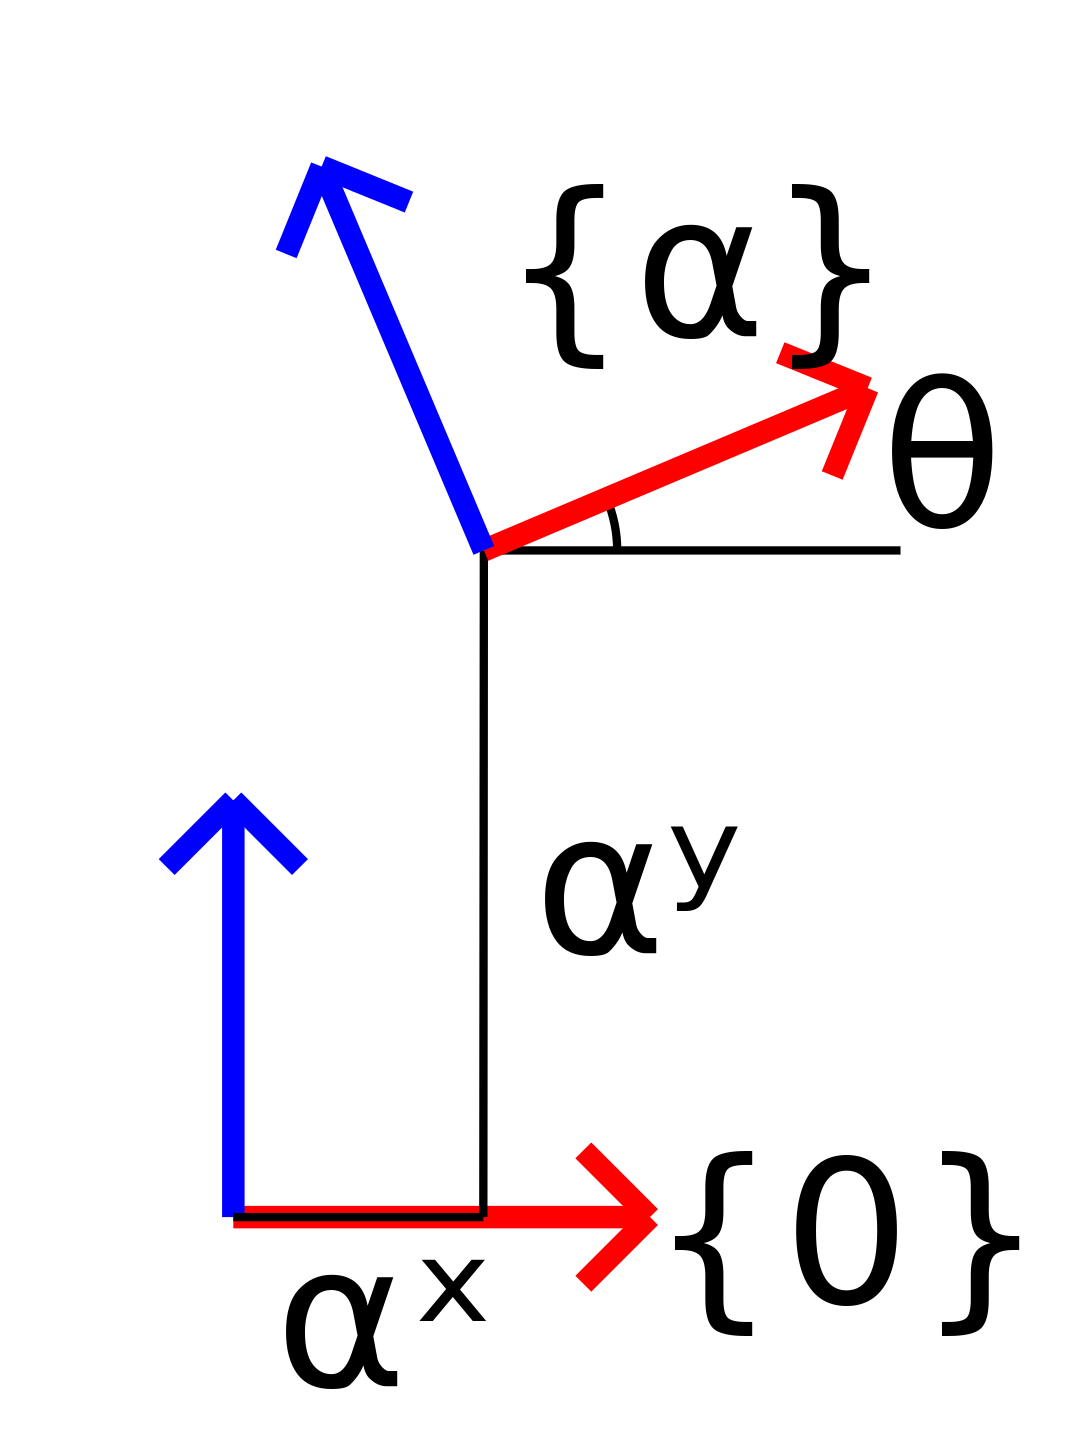
\includegraphics[scale=0.1]{generated_figures/frames_4c.png}
        \end{center}
        %Let $\theta = \frac\pi4$. 
        \begin{enumerate} [label=(\roman*)]
          \item What is $H_\alpha^0$?
          \item $p^\alpha = \begin{bmatrix} 0 \\ 0 \end{bmatrix}$
          
          %\item \transform{q}{}{\alpha} = \smcolvec{1\\0}
          \item $q^\alpha = \begin{bmatrix} 1 \\ 0 \end{bmatrix}$
          
          %\item \transform{v}{}{\alpha} = \smcolvec{0\\1}
          \item $v^\alpha = \begin{bmatrix} 0 \\ 1 \end{bmatrix}$
          
          %\item \transform{u}{}{\alpha} = \smcolvec{1\\1}
          \item $u^\alpha = \begin{bmatrix} 1 \\ 1 \end{bmatrix}$
          
        \end{enumerate}
        \noindent Ensure that the coordinates make sense in the
        new representation.

        \begin{tcolorbox}[height=3cm]
         % TODO: ENTER YOUR ANSWER HERE
        \end{tcolorbox}

        \setcounter{partno}{3}

        \item \text{[5 point]}
        Find $H_\beta^0$, using the frames shown in the figure.
        \begin{center}
        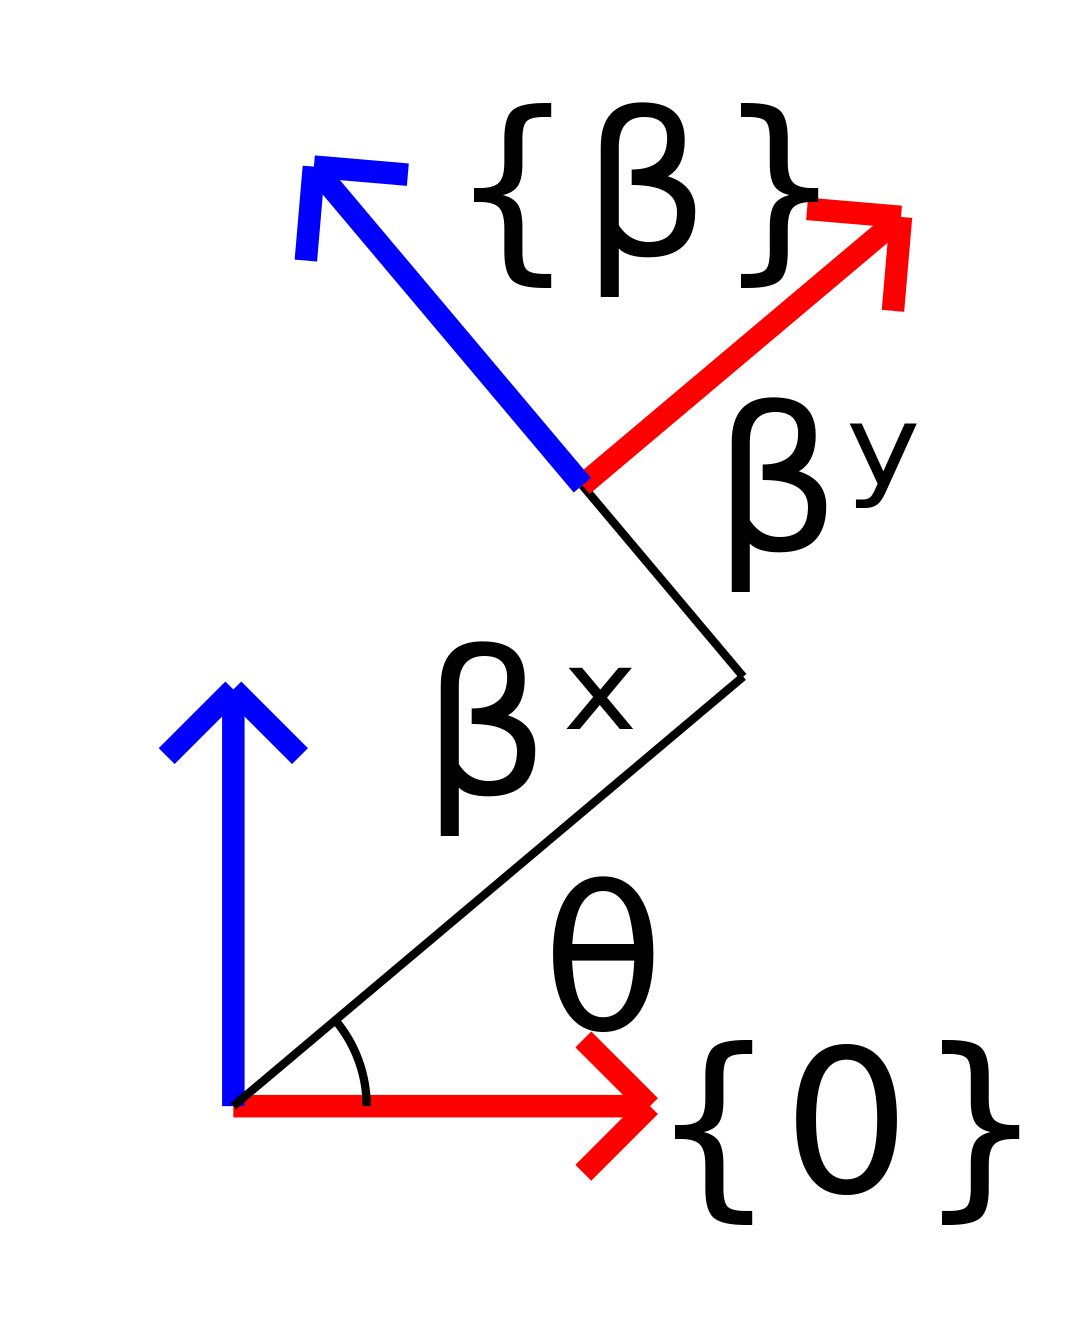
\includegraphics[scale=0.1]{generated_figures/frames_4d.png}
        \end{center}
        Let $\theta=\frac\pi4$. Verify your solution by using this matrix to transform the following
        points $p, q$ and vectors $v, u$ (given in \frame{\beta})  to \frame{0})
        \begin{enumerate} [label=(\roman*)]
          \item $p^\beta = \begin{bmatrix} 0 \\ 0 \end{bmatrix}$
          
          % \item \transform{q}{}{\beta} = \smcolvec{1\\0}
          \item $q^\beta = \begin{bmatrix} 1 \\ 0 \end{bmatrix}$
          
          	% \item \transform{v}{}{\beta} = \smcolvec{0\\1}
           \item $v^\beta = \begin{bmatrix} 0 \\ 1 \end{bmatrix}$
          	
          	% \item \transform{u}{}{\beta} = \smcolvec{1\\1}
           \item $u^\beta = \begin{bmatrix} 1 \\ 1 \end{bmatrix}$
          	
        \end{enumerate}
        \noindent Ensure that the coordinates make sense in the
        new representation.

        \begin{tcolorbox}[height=3cm]
         % TODO: ENTER YOUR ANSWER HERE
        \end{tcolorbox}

        \item \text{[1 point]} 
        Find $H_\beta^\alpha$. %\H{\beta}{\alpha}.

        \begin{tcolorbox}[height=3cm]
         % TODO: ENTER YOUR ANSWER HERE
        \end{tcolorbox}


        \item \text{[2 points]} 
        Compute $H_\alpha^0$ and $(H_\alpha^0)^{-1}$.
        %Compute \H{\alpha}{0} and \inv{\H{\alpha}{0}}. 
        Verify that
        %(\inv{\H{\alpha}{0}} \H{\alpha}{0}) = \smcolvec{1&0&0\\0&1&0\\0&0&1}.
        $(H_\alpha^0)^{-1} H_\alpha^0 = I_{3\times3}.$

        \begin{tcolorbox}[height=3cm]
         % TODO: ENTER YOUR ANSWER HERE
        \end{tcolorbox}

        
    \end{enumerate}

    \titledquestion{\textbf{Workspace and Frames}}[8]
    \textbf{Before continuing, please read over the appendix.}
    Consider the following robot:

    \begin{center}
    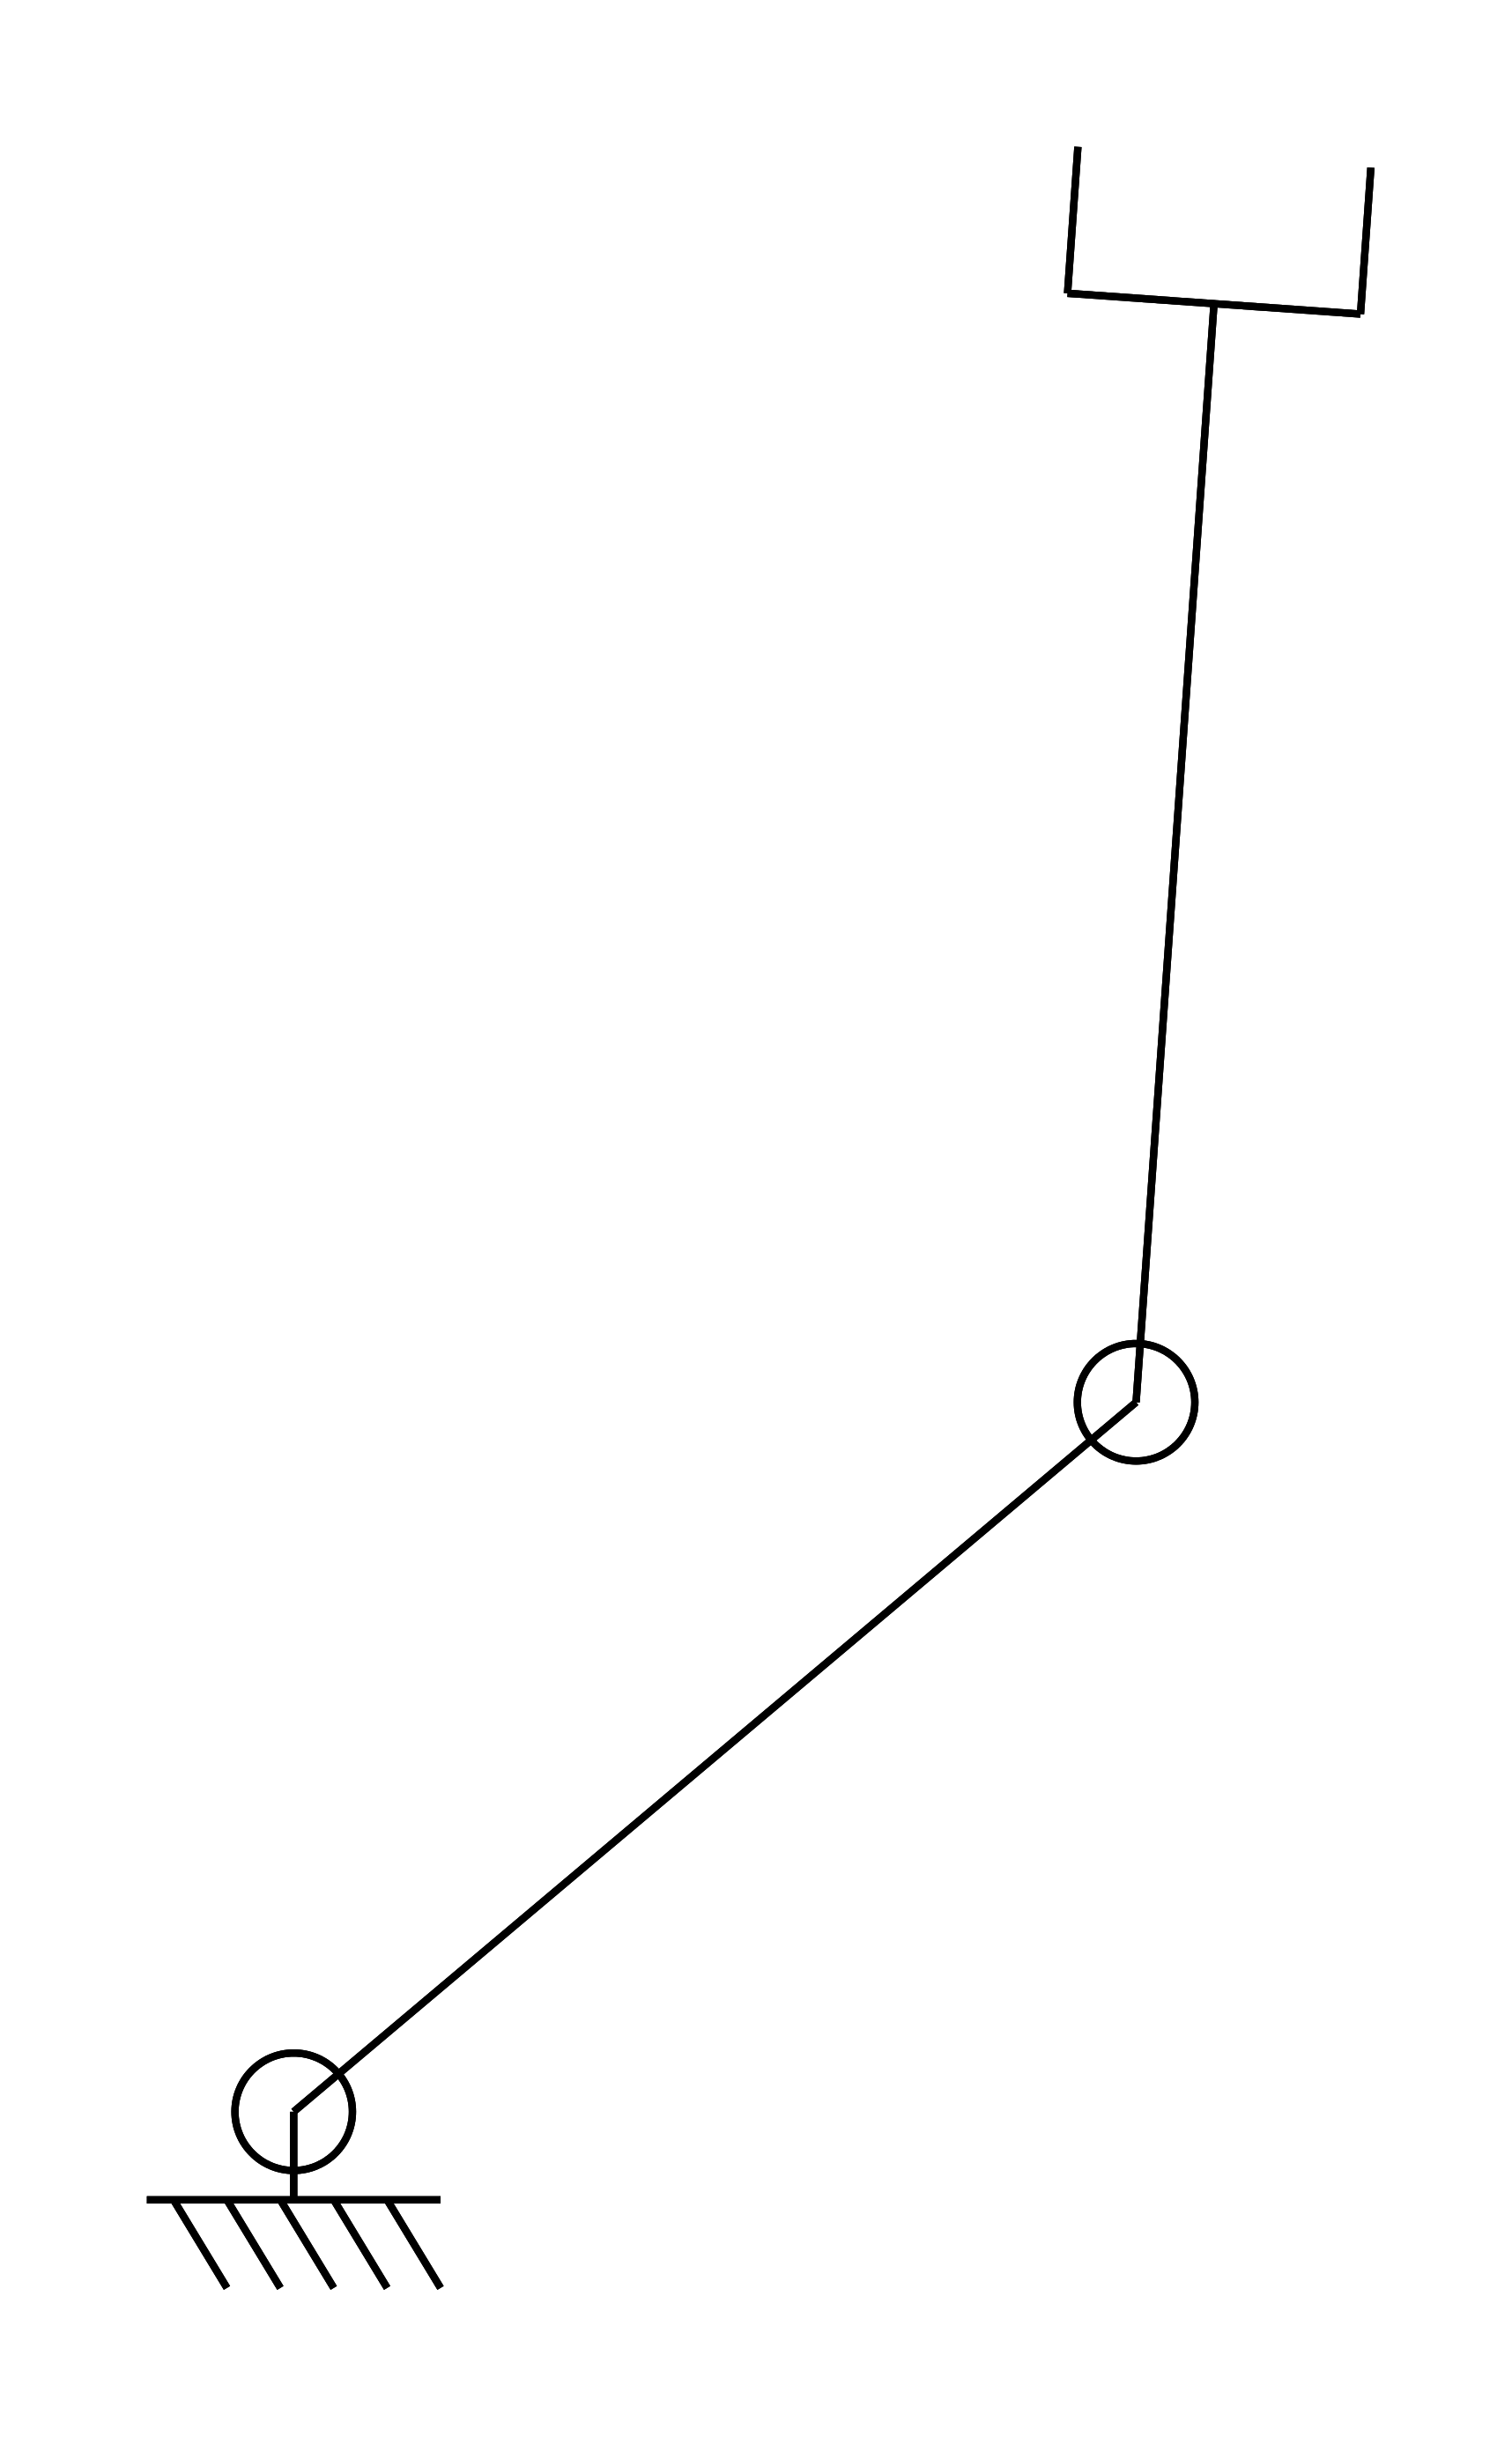
\includegraphics[width=1.5in]{generated_figures/robot_5.png}
    \end{center}

    Draw and clearly label the following, \textbf{using the frame conventions given in
    the background for this assignment}.
    \begin{enumerate}[label=\alph*.]
        \item \text{[1 point]} The base frame of the entire robot: \frame{0}.
        \begin{tcolorbox}[height=3cm]
         % TODO: ENTER YOUR ANSWER HERE
        \end{tcolorbox}
        \item \text{[1 point]} The starting frame for the first link: \frame{1}
        \begin{tcolorbox}[height=3cm]
         % TODO: ENTER YOUR ANSWER HERE
        \end{tcolorbox}
        \item \text{[1 point]} The frame at the end of the first link: \frame{2}
        \begin{tcolorbox}[height=3cm]
         % TODO: ENTER YOUR ANSWER HERE
        \end{tcolorbox}
        \item \text{[1 point]} The starting frame for the second link: \frame{3}
        \begin{tcolorbox}[height=3cm]
         % TODO: ENTER YOUR ANSWER HERE
        \end{tcolorbox}
        \item \text{[1 point]} The end effector frame: \frame{4}
        \begin{tcolorbox}[height=3cm]
         % TODO: ENTER YOUR ANSWER HERE
        \end{tcolorbox}
        
        
        \item \text{[3 points]} Assume $l_1 > l_2$. On a separate plot, shade the workspace (in
        $\RR^2$), ignoring self-collision. Label the dimensions of this plot.
        \begin{tcolorbox}[height=3cm]
         % TODO: ENTER YOUR ANSWER HERE
        \end{tcolorbox}

        
    \end{enumerate}

    \titledquestion{\textbf{Forward Kinematics of an RR Arm}}[9]
    For the robot in the previous question, compute the following in terms of
    $l_1$, $l_2$, $\theta_1$, and $\theta_2$:

    \begin{enumerate}[label=\alph*.]
        \item \text{[1 point]} $H_1^0$
        \begin{tcolorbox}[height=3cm]
         % TODO: ENTER YOUR ANSWER HERE
        \end{tcolorbox}
        
        \item \text{[1 point]} $H_2^1$
        \begin{tcolorbox}[height=3cm]
         % TODO: ENTER YOUR ANSWER HERE
        \end{tcolorbox}
        
        \item \text{[1 point]} $H_3^2$
        \begin{tcolorbox}[height=3cm]
         % TODO: ENTER YOUR ANSWER HERE
        \end{tcolorbox}

        \item \text{[1 point]} $H_4^3$
        \begin{tcolorbox}[height=3cm]
         % TODO: ENTER YOUR ANSWER HERE
        \end{tcolorbox}
        
        \item \text{[1 point]} $H_4^0$, the transform from the end effector to the base frame (using the previous transforms).

        \begin{tcolorbox}[height=3cm]
         % TODO: ENTER YOUR ANSWER HERE
        \end{tcolorbox}
        
        \item  The position of the origin of the end effector frame
        \frame{4}, represented in the base frame \frame{0}, for the following
        values of $\begin{bmatrix} \theta_1 \\ \theta_2 \end{bmatrix}$. %\smcolvec{\th[1]\\\th[2]}. 
        Solving for both
        ``nice'' numbers and intermediate numbers will build 
        intuition of RR arm forward kinematics.
        \begin{enumerate} [label=(\roman*)]
            \item \text{[1 point]} $\begin{bmatrix}0\\0\end{bmatrix}$ %\smcolvec{0\\0}
 
            \item \text{[1 point]} $\begin{bmatrix}0 \\ \frac\pi2 \end{bmatrix}$ %\smcolvec{0\\\piover{2}}
       
            \item \text{[1 point]} $\begin{bmatrix}
                \frac\pi2 \\ -\frac\pi2
            \end{bmatrix}$ %\smcolvec{\piover{2}\\-\piover{2}}
            
            \item \text{[1 point]} $\begin{bmatrix}
                \frac\pi3 \\ \frac\pi2
            \end{bmatrix}$ %\smcolvec{\piover{3}\\\piover{2}}
    
        \end{enumerate}
        \begin{tcolorbox}[height=3cm]
         % TODO: ENTER YOUR ANSWER HERE
        \end{tcolorbox}
    \end{enumerate}

    \titledquestion{\textbf{Workspace and Frames of a PR Arm}}[8]
    Repeat problem 8 for the following arm:

    \begin{center}
    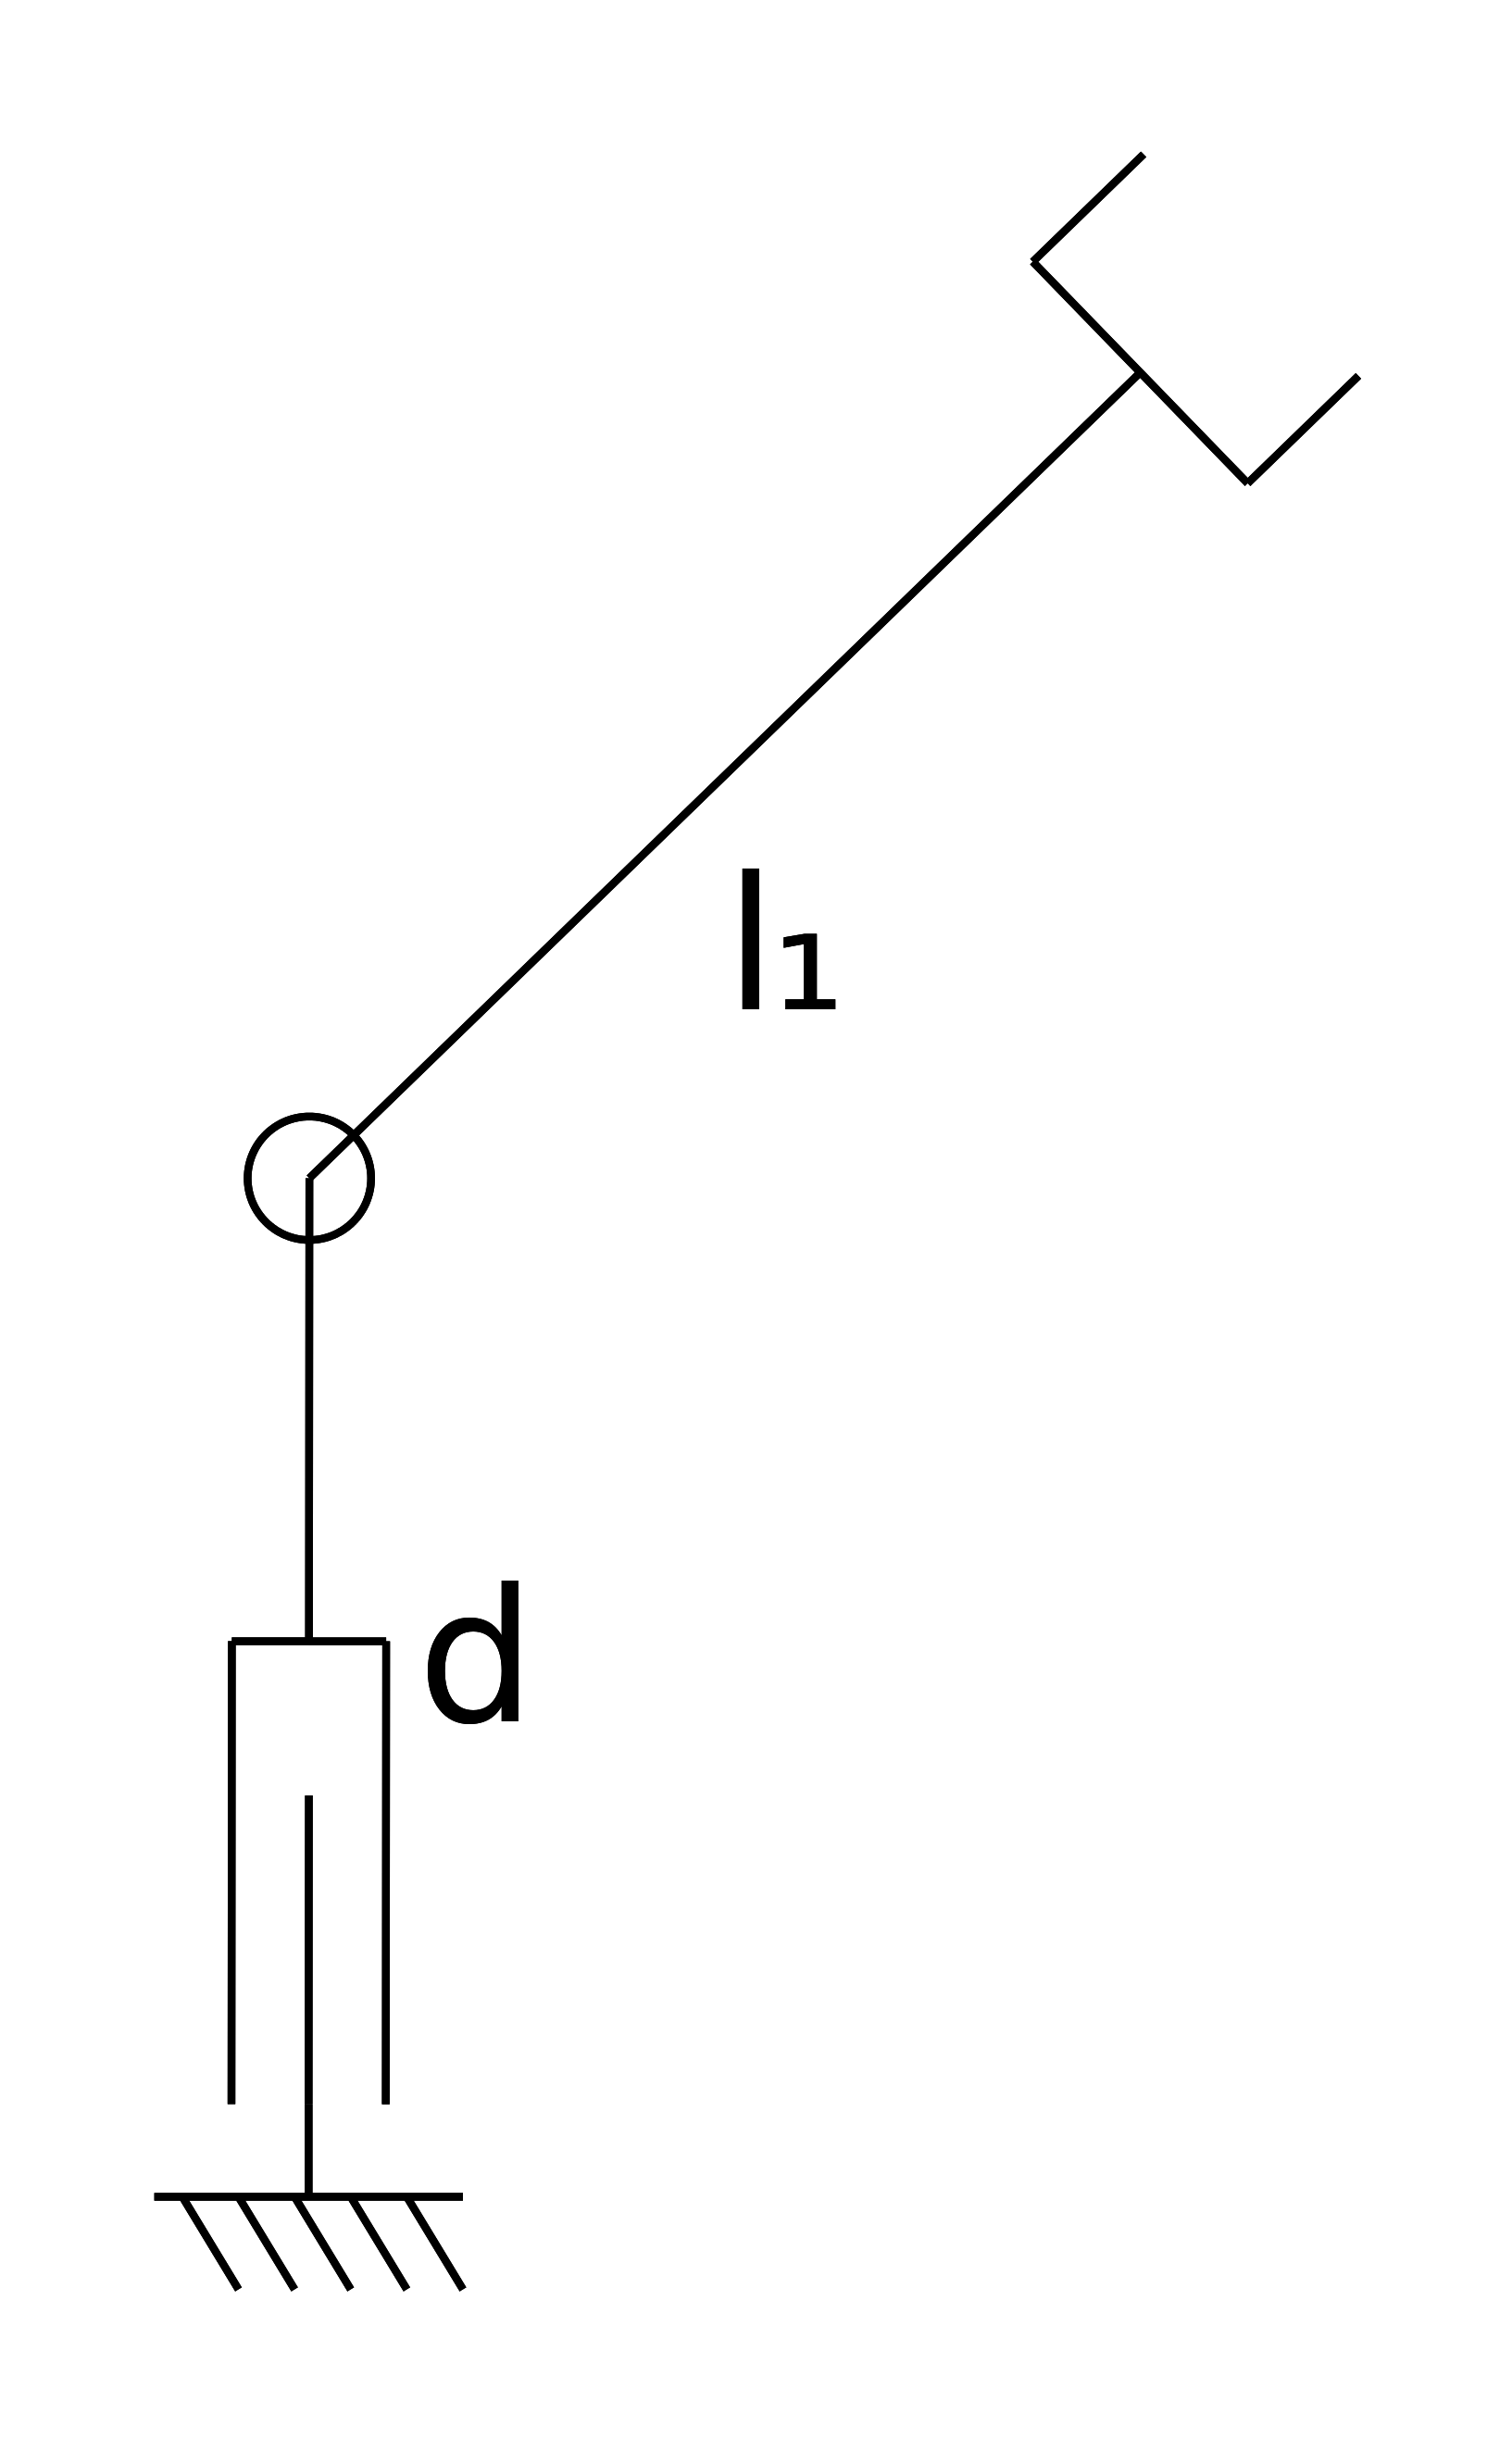
\includegraphics[width=1.5in]{generated_figures/robot_7.png}
    \end{center}
    Remember to use the frame conventions given in the background!
    \begin{enumerate}[label=\alph*.]
    \item \text{[1 point]} The base frame of the entire robot: \frame{0}.
    \begin{tcolorbox}[height=3cm]
         % TODO: ENTER YOUR ANSWER HERE
    \end{tcolorbox}
    \item \text{[1 point]} The starting frame for the first link: \frame{1}
    \begin{tcolorbox}[height=3cm]
         % TODO: ENTER YOUR ANSWER HERE
    \end{tcolorbox}
    \item \text{[1 point]} The frame at the end of the first link: \frame{2}
    \begin{tcolorbox}[height=3cm]
         % TODO: ENTER YOUR ANSWER HERE
    \end{tcolorbox}
    \item \text{[1 point]} The starting frame for the second link: \frame{3}
    \begin{tcolorbox}[height=3cm]
         % TODO: ENTER YOUR ANSWER HERE
    \end{tcolorbox}
    \item \text{[1 point]} The end effector frame: \frame{4}
    \begin{tcolorbox}[height=3cm]
         % TODO: ENTER YOUR ANSWER HERE
    \end{tcolorbox}
        
    \item \text{[3 points]} For the workspace, assume the prismatic joint can go from $d=0$ to $d=d_f$. Draw a separate image for $d_f = l_1$ and $d_f > 2 l_1$.
    \begin{tcolorbox}[height=3cm]
         % TODO: ENTER YOUR ANSWER HERE
    \end{tcolorbox}
        
    \end{enumerate}

    \titledquestion{\textbf{Forward Kinematics of a PR Arm}}[9]
    Repeat problem 9 with the PR arm in problem 10.

    \begin{enumerate} [label=\alph*.]
        \item \text{[1 point]} $H_1^0$ % \H{1}{0}
        \begin{tcolorbox}[height=3cm]
         % TODO: ENTER YOUR ANSWER HERE
        \end{tcolorbox}

        \item \text{[1 point]} $H_2^1$ % \H{2}{1}
        \begin{tcolorbox}[height=3cm]
         % TODO: ENTER YOUR ANSWER HERE
        \end{tcolorbox}
        
        \item \text{[1 point]} $H_3^2$ % \H{3}{2}
        \begin{tcolorbox}[height=3cm]
         % TODO: ENTER YOUR ANSWER HERE
        \end{tcolorbox}
        
        \item \text{[1 point]} $H_4^3$ % \H{4}{3}
        \begin{tcolorbox}[height=3cm]
         % TODO: ENTER YOUR ANSWER HERE
        \end{tcolorbox}
        
        \item \text{[1 point]} $H_4^0$, the transform from the end effector to the base frame (using the previous transforms).
        \begin{tcolorbox}[height=3cm]
         % TODO: ENTER YOUR ANSWER HERE
        \end{tcolorbox}


    \item \text{[4 points]} The position of the origin of the end effector frame \frame{4}, represented in the base frame \frame{0}, for the following values of
    $\begin{bmatrix} d \\ \theta \end{bmatrix}$. Solving for both ``nice'' numbers and intermediate numbers will build 
    intuition of PR arm forward kinematics.

        \begin{enumerate} [label=(\roman*)]
            \item $\begin{bmatrix} 0 \\ 0 \end{bmatrix}$ %\smcolvec{0\\0}

            \item $\begin{bmatrix} 3 \\ \frac\pi2 \end{bmatrix}$ %\smcolvec{3\\\piover{2}}

             \item $\begin{bmatrix} 1 \\ -\frac\pi2 \end{bmatrix}$ %\smcolvec{1\\-\piover{2}}

            \item $\begin{bmatrix} 3 \\ \frac\pi4 \end{bmatrix}$ % \smcolvec{3\\\piover{4}}

        \end{enumerate}
        \begin{tcolorbox}[height=3cm]
         % TODO: ENTER YOUR ANSWER HERE
        \end{tcolorbox}
        
    \end{enumerate}


    \titledquestion{\textbf{Singularities}}[8]
    Consider the following RR arm:
    \begin{center}
    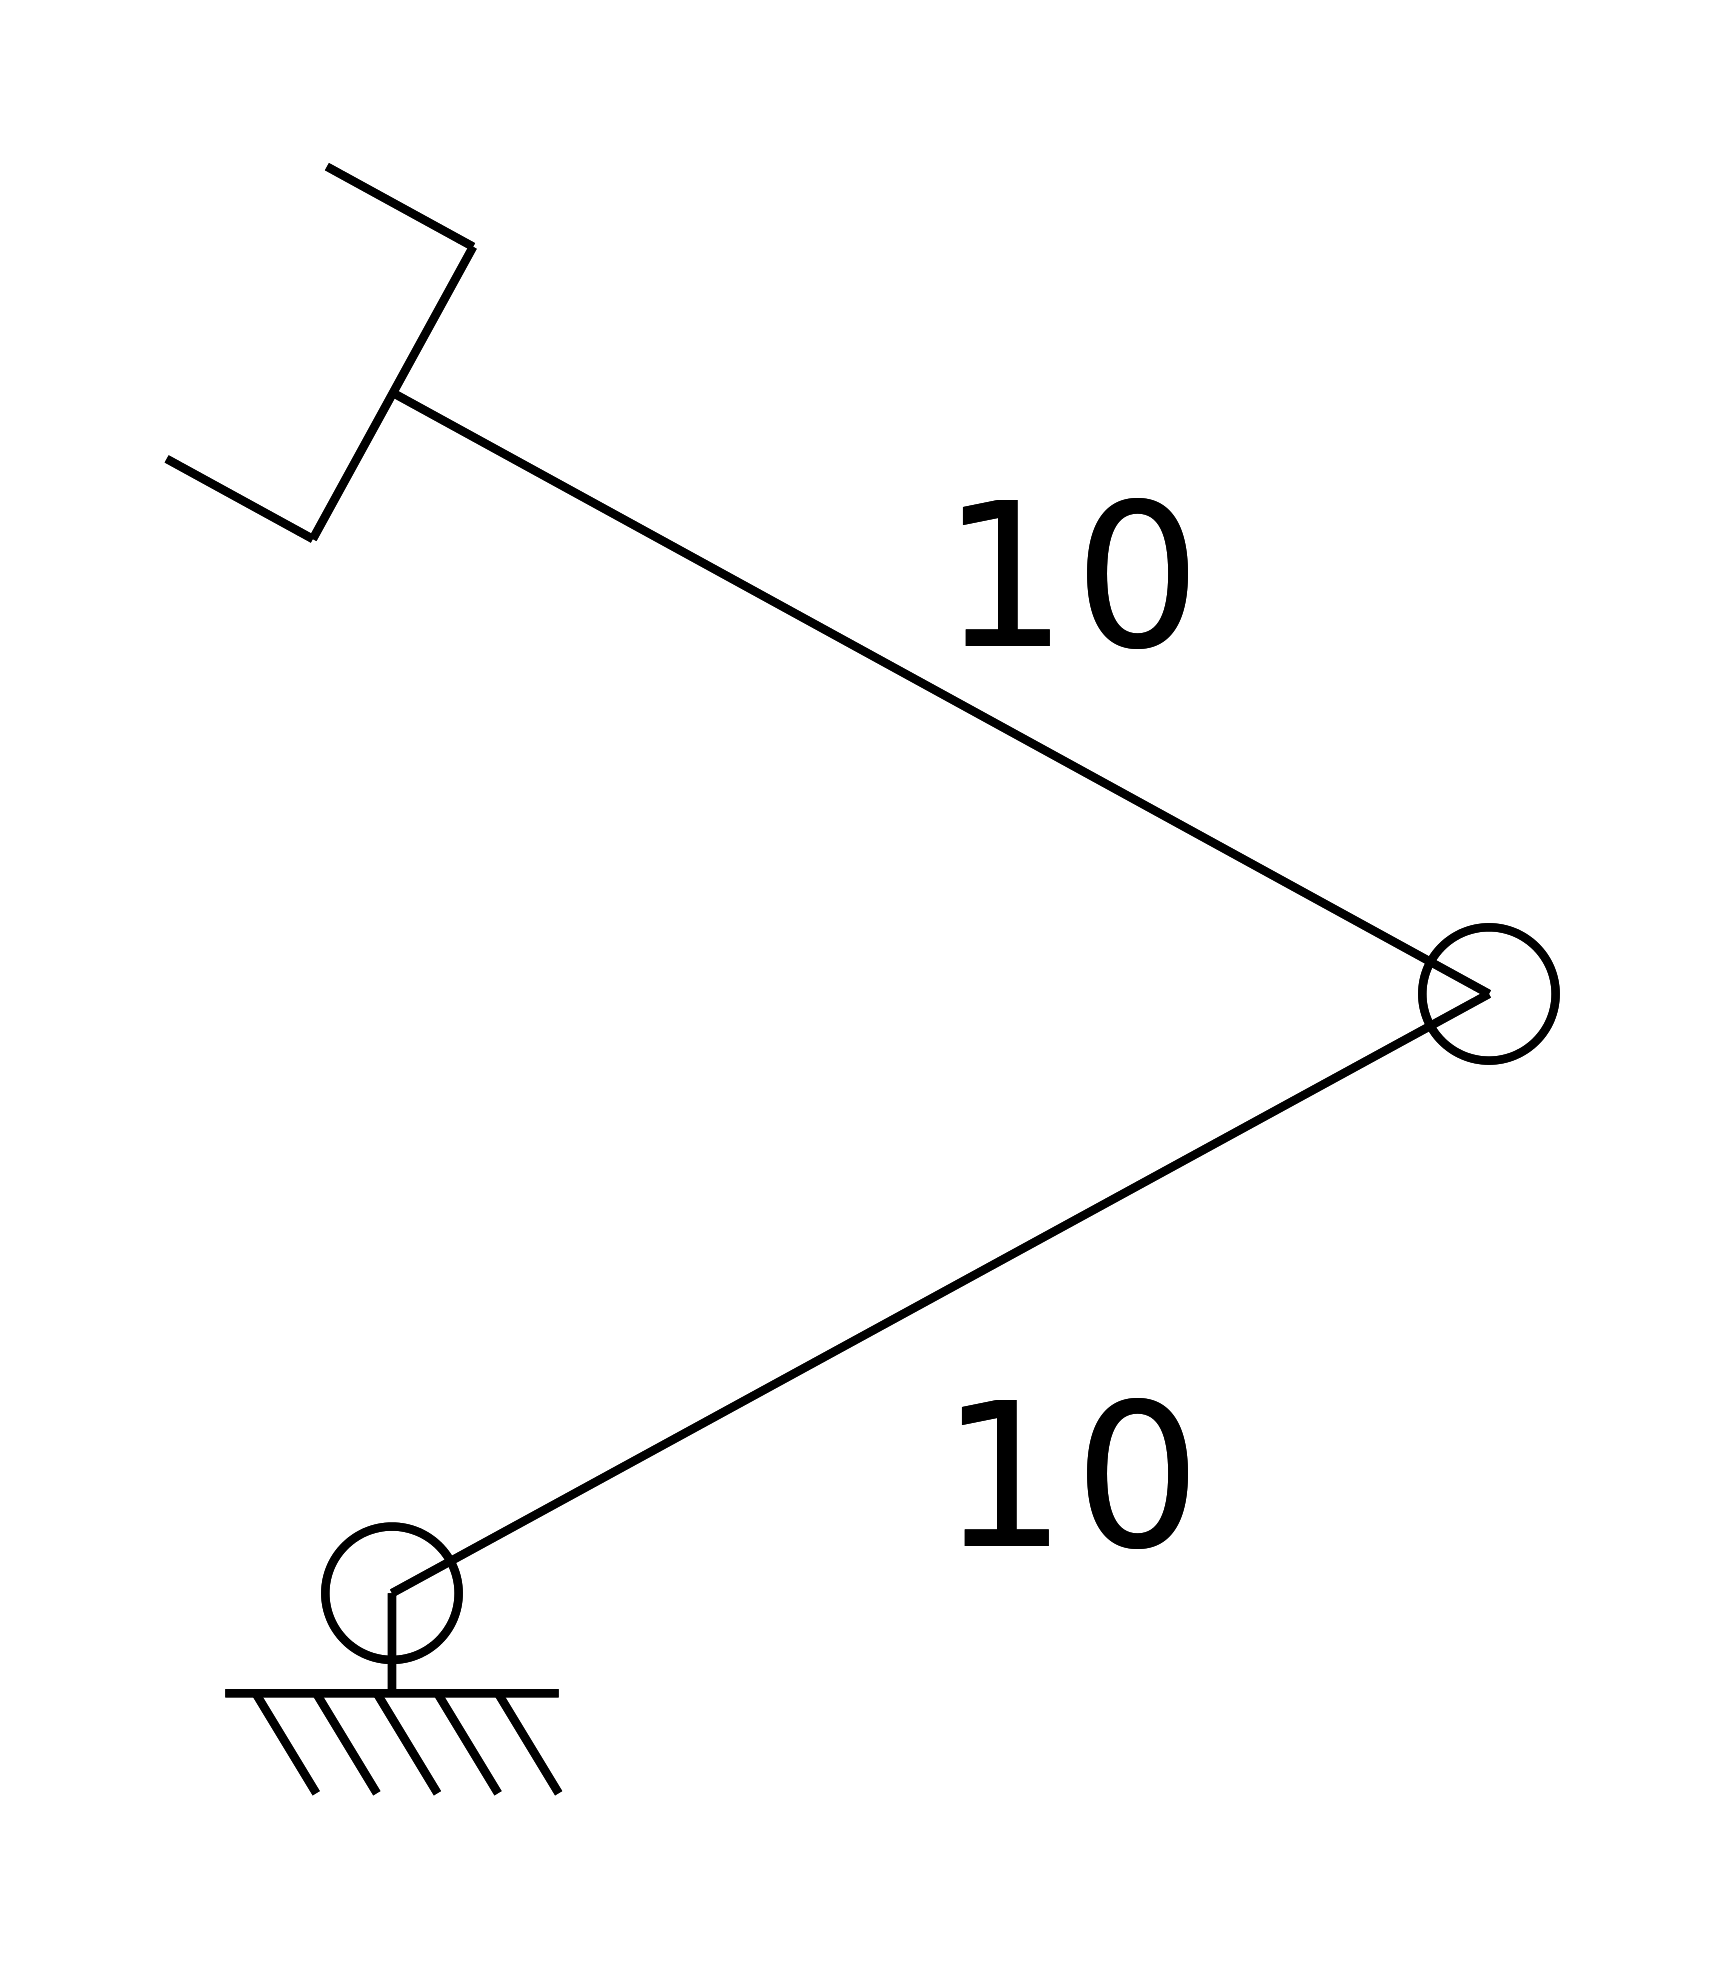
\includegraphics[width=1.5in]{generated_figures/robot_8.png}
    \end{center}

    Draw labeled plots. Please draw each part separately.

    For which $\begin{bmatrix} x \\ y \end{bmatrix}$ or set of $\begin{bmatrix} x \\ y \end{bmatrix}$%\smcolvec{x\\y} 
    in the workspace can the solution 
    $\theta = \begin{bmatrix} \theta_1 \\ \theta_2 \end{bmatrix}$ have
    %\th=\smcolvec{\th[1]\\\th[2]}~have:
    \begin{enumerate} [label=\alph*.]
        \item \text{[2 points]} Only 1 value?
        \begin{tcolorbox}[height=3cm]
         % TODO: ENTER YOUR ANSWER HERE
        \end{tcolorbox}

        \item \text{[2 points]} Exactly 2 values?
        \begin{tcolorbox}[height=3cm]
         % TODO: ENTER YOUR ANSWER HERE
        \end{tcolorbox}
        
        \item \text{[4 points]} Infinite values?
        \begin{tcolorbox}[height=3cm]
         % TODO: ENTER YOUR ANSWER HERE
        \end{tcolorbox}

            
    \end{enumerate}

    

\end{questions}

\begin{submissionChecklist}
		\item Create a PDF of your answers to the written questions with the name \verb!<andrew_id>.pdf! and submit it to Gradescope.
       	\item For the code section that will be released, run \verb!create_submission.py! in the python terminal.
       	\item Upload \verb!<andrew_id>.zip! to Gradescope.
        \item Coding questions are autograded, with no limit on number of submissions within the mandated deadline.
 
	\end{submissionChecklist}

 \newpage
 \section{Summary of concepts}

 \subsection{Preliminary Terms}

\define{Coordinate Frame}{
    A coordinate frame consists of a special point called the \emph{origin} and 
    some number of orthonormal\footnotemark~axes.  Frames provide a reference for
    measurements of positions and rotations of a body or point.  
    Frame \vec{i} is denoted \frame{i}. For the purposes of this class, all frames 
    must be right-handed.
}

\footnotetext{
Orthonormal axes are:
\begin{itemize}
    \item unit vectors (length 1)
    \item mutually orthogonal (perpendicular to each other)
\end{itemize}
}

\define{Point}{
    A point is a fixed position in space. Its coordinates depend on the frame describing
    it. Point \vec{p} relative to \frame{0} is denoted \p{0}. For example,
    in the figure below $\p{0} = \smcolvec{2\\1}$ and $\p{1} = \smcolvec{-1\\2}$.
}
\begin{center}
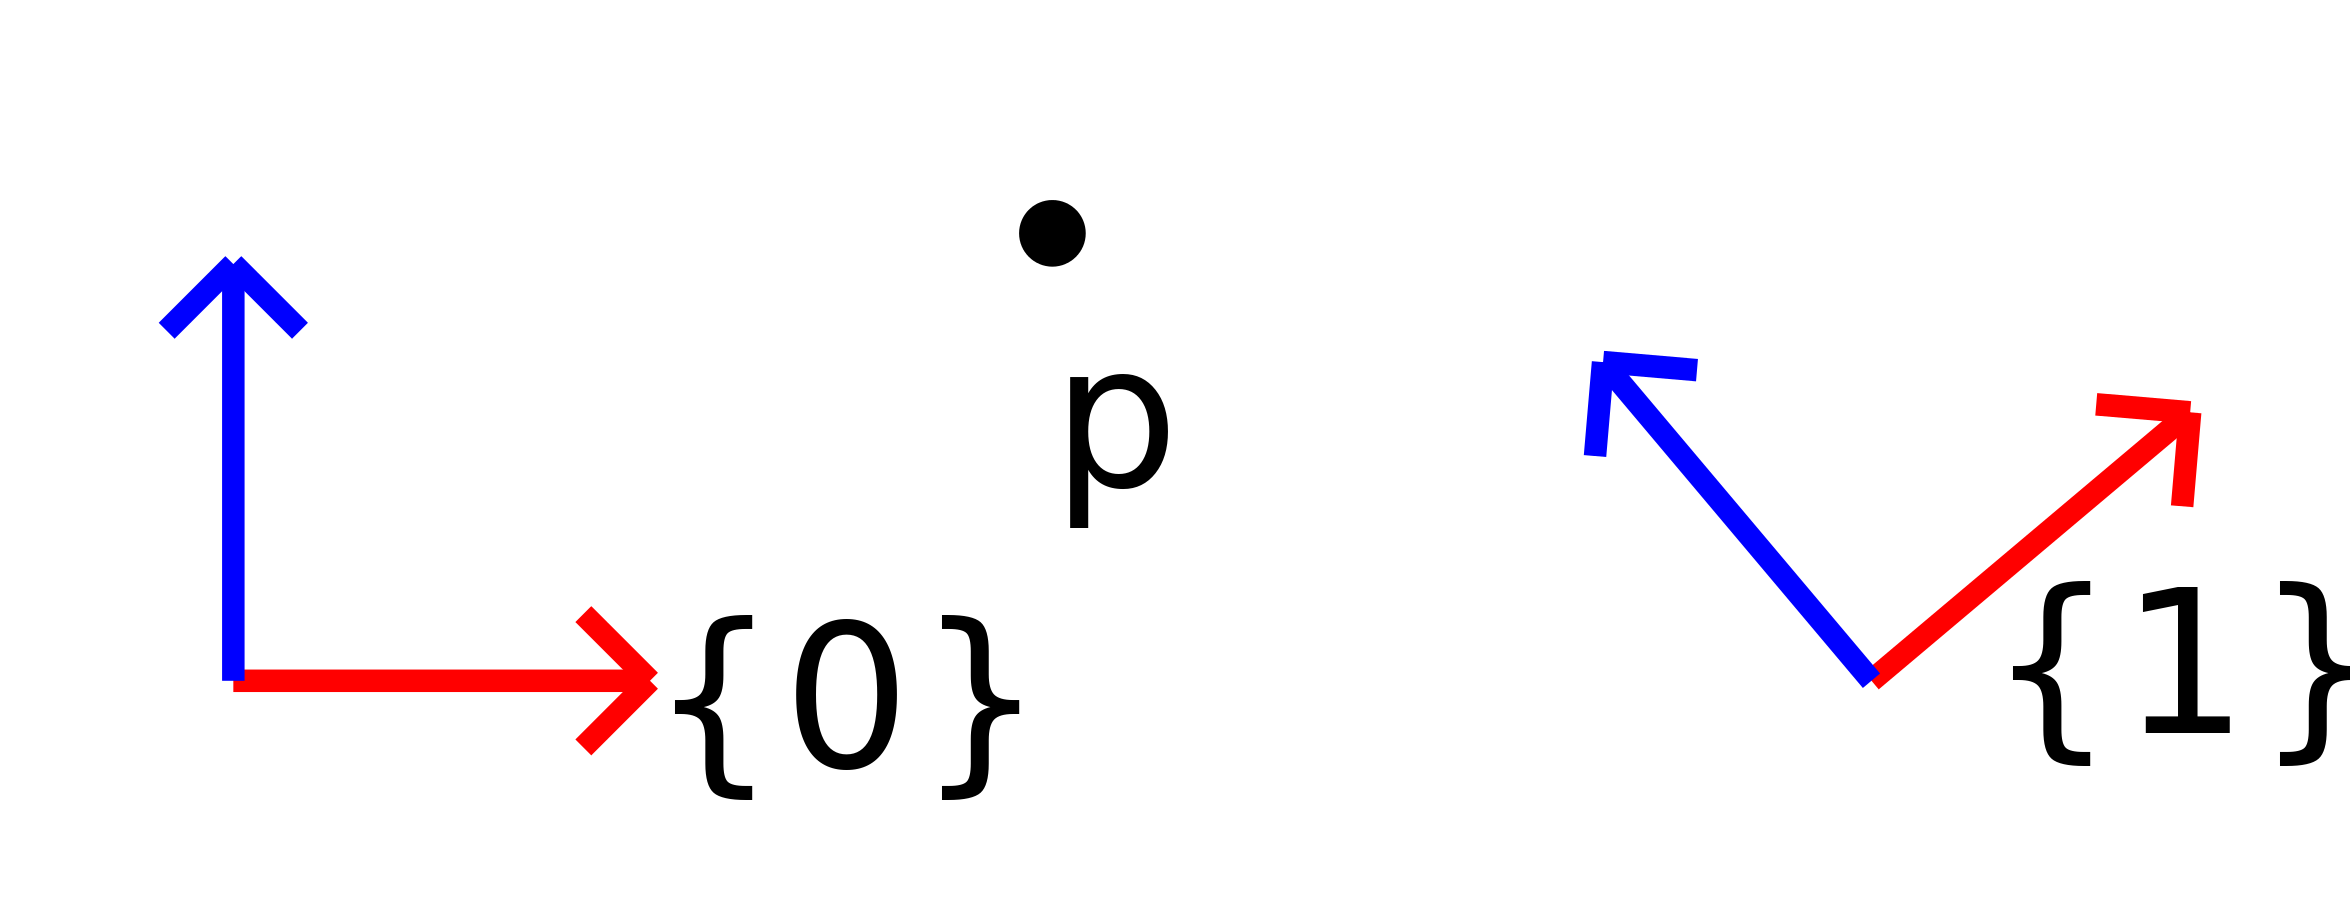
\includegraphics[scale=0.1]{generated_figures/frames_bg_pt.png}
\end{center}

\define{Vector}{
    A direction and magnitude that is free in space.  Among other things,
    vectors can describe offsets from a point, forces, or velocities. Just like a point, the
    direction of the vector depends upon in which frame it is referenced, but the magnitude
    remains constant in all frames. For example, in the figure below $\v{0} = \smcolvec{.7071\\-.
    7071}$ and $\v{1} = \smcolvec{0\\-1}$ both have a magnitude of 1.  
}
\begin{center}
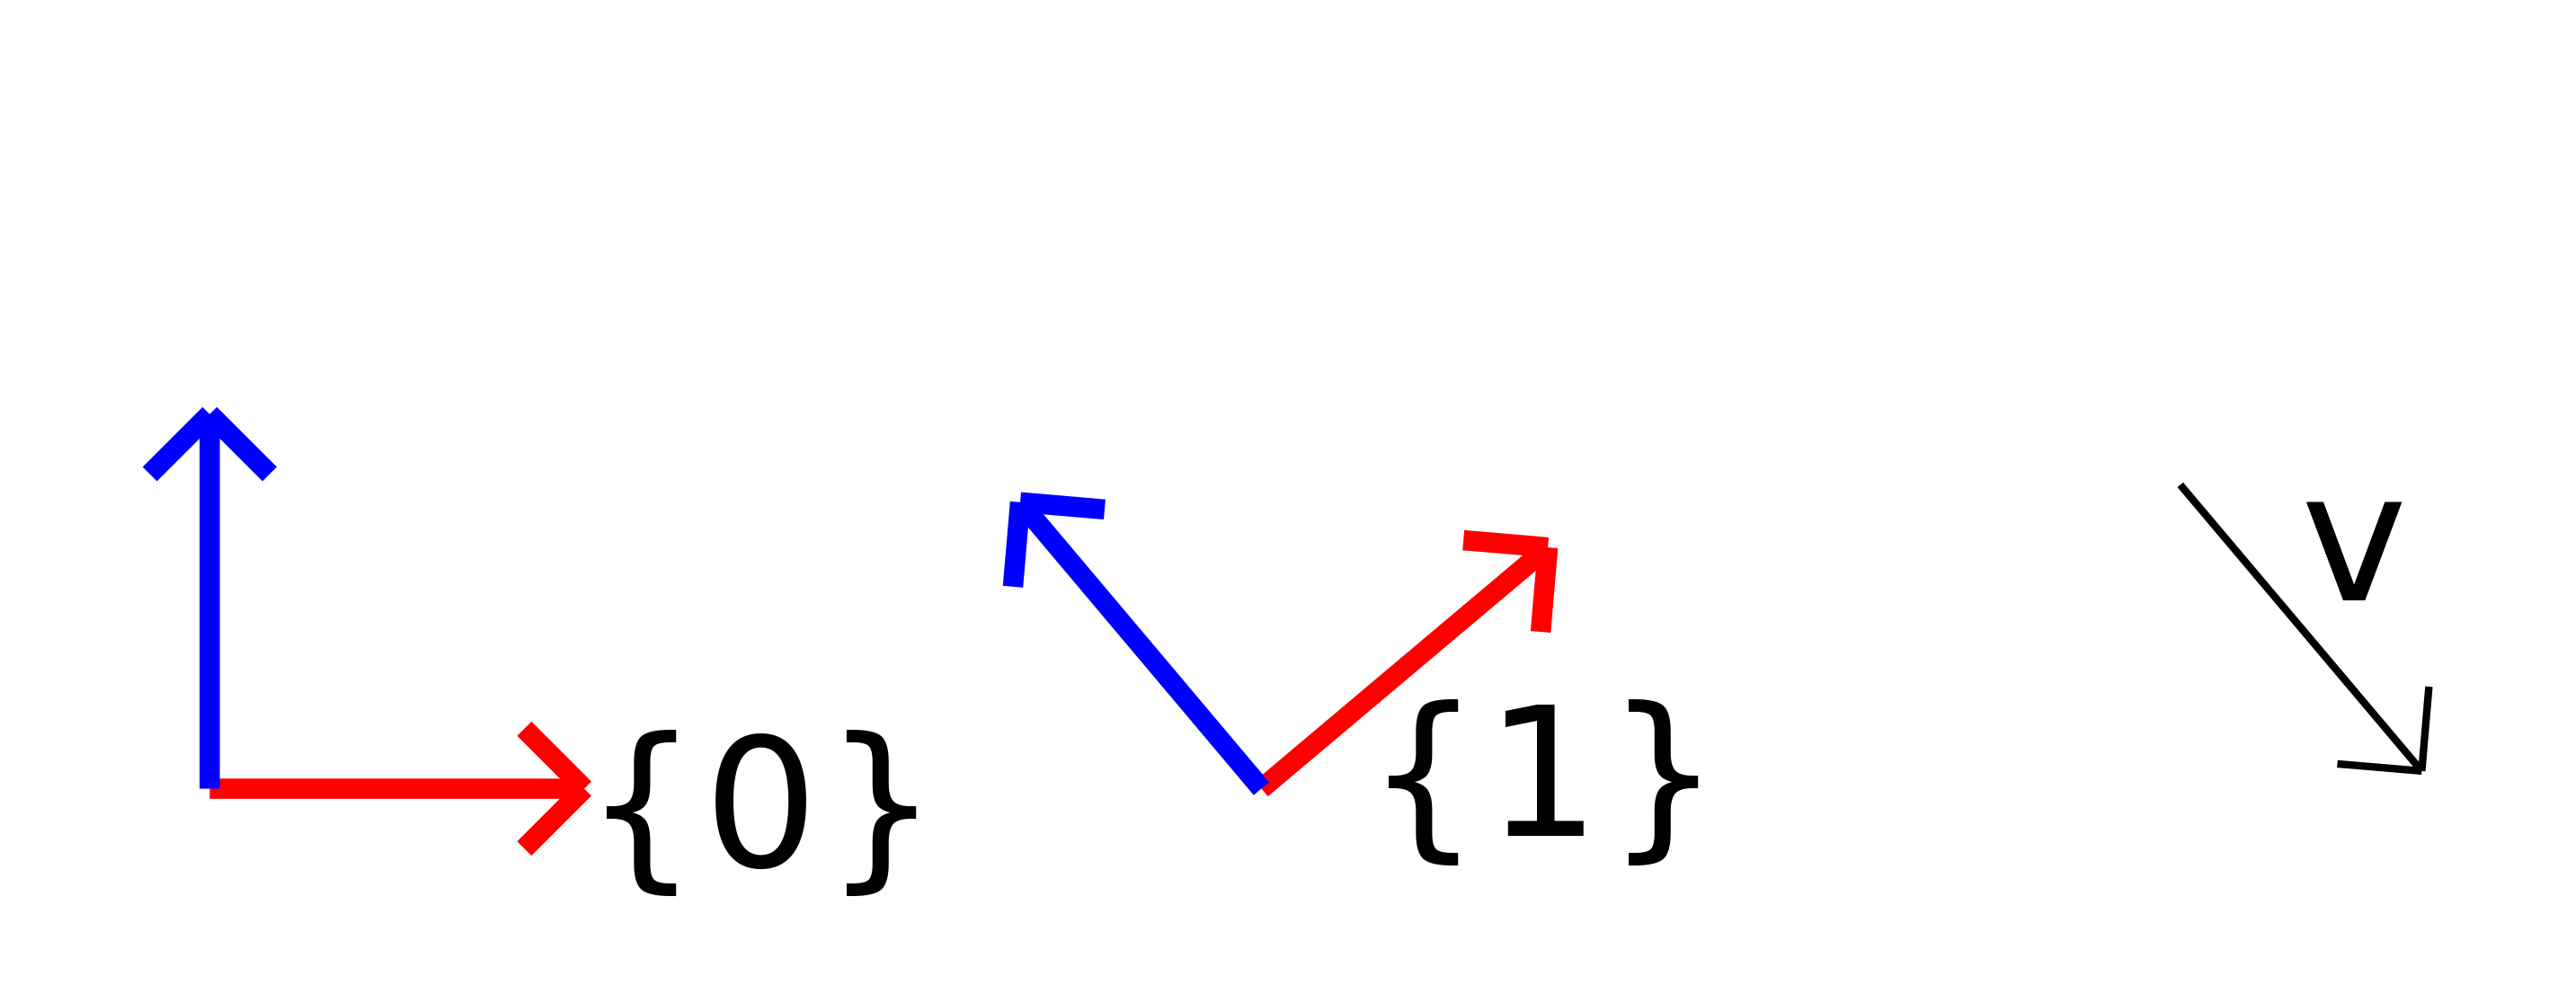
\includegraphics[scale=0.1]{generated_figures/frames_bg_vec.png}
\end{center}

\define{Rigid Body}{
    A collection of points where the distance between two points and the handedness of the points
    remains constant while the collection undergoes a displacement. 
}

\define{Rigid Motion}{
    A translation, rotation, or combination of the two that can be applied to
    a body without changing the distance between any two points in the body or 
    changing the handedness of the points.
}

\define{$\RR^2$}{
    Two-dimensional Cartesian space; can be parameterized by $x$ and $y$.
}

\define{SE(2)} {
    It is both 1) the space corresponding to position and orientation of a rigid body in two
    dimensions and 2) the set of rigid motions in two dimensions.
    It is usually parameterized by $x$, $y$, and $\theta$.
}

\define{Workspace}{
    The set of all points \p{} such that there exists
    some joint configuration which places a robot's end effector at \p{}.
}

\subsection{Robots and Robot Diagrams}

For the purpose of this class, a \textbf{robot} or a \textbf{linkage} is a
combination of \emph{links} (which are rigid bodies) and \emph{joints}, which
connect two links with a certain constraint on relative motion. Links are
generally represented by straight lines in robot diagrams. The two
categories of joints we will use in this class are \emph{rotational} and
\emph{prismatic} joints.

\define{Revolute Joint}{
    Creates an angular offset between two adjacent links.  This offset is
    typically notated as $\theta$, with a subscript that matches the joint index
    or name.  Positive rotations go from the x axis towards the y axis (i.e.,
    they follow the right hand rule). They are drawn as follows in robot
    diagrams: 
}
\begin{center}
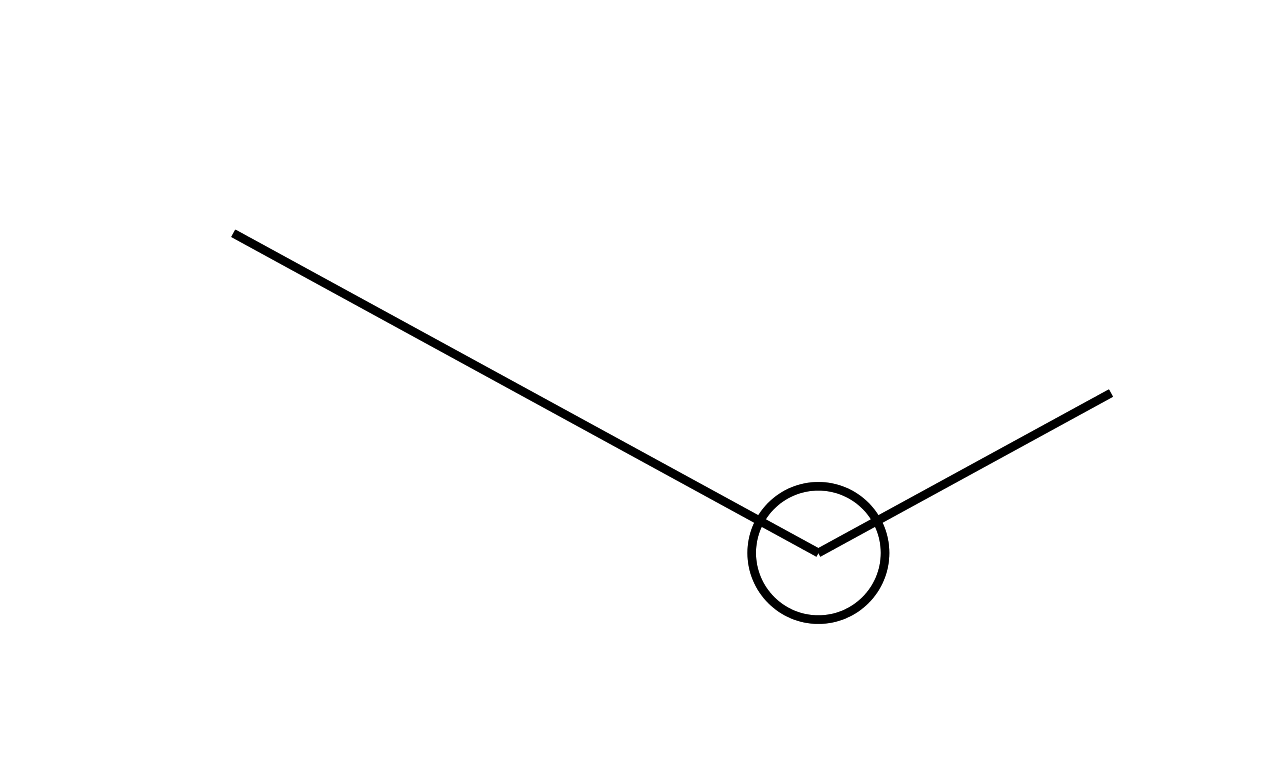
\includegraphics[width=1.5in]{generated_figures/bg_rot_joint_diagram.png}
\end{center}

\define{Prismatic Joint}{
    Creates a translational offset between two adjacent links along a single axis. The notation
    for this offset varies. We will refer to this as $d$ with a subscript to match the joint
    index or name, but in a robot with both rotational and prismatic joints sometimes $\theta or
    q$ is used for any joint.  They are drawn as follows in robot diagrams.
    Note that this figure represents two separate links with one prismatic joint
    in between with a total length is $l_1 + l_2 + d$; however, depending on the
    system, $l_1$ and $l_2$ may be omitted and just combined into $d$. You can use either
    convention, but be sure to label any diagrams clearly.
}

\begin{center}
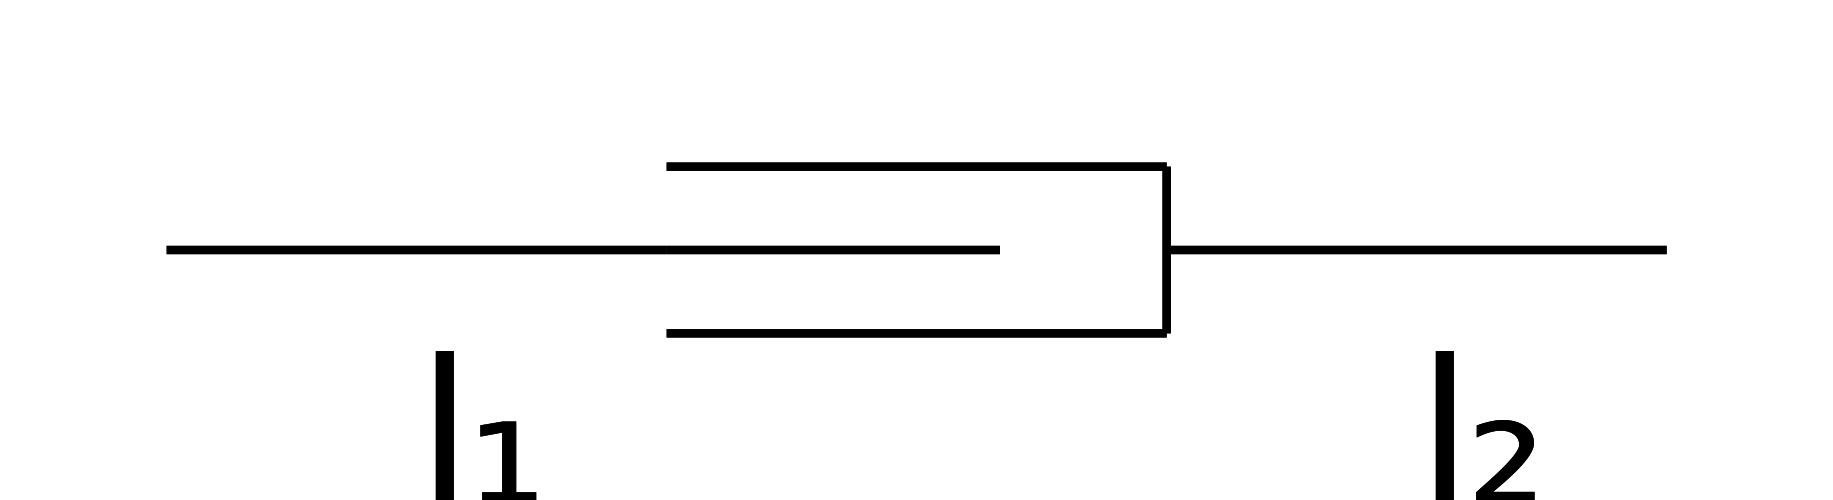
\includegraphics[width=1.5in]{generated_figures/bg_prism_joint_diagram.png}
\end{center}

\define{Kinematic Chain}{
    An $n$-joint kinematic chain is a robot consisting of $n+1$ links and $n$ joints, connected
    in series.  If the robot is attached to the world, the first link is called the base link.
    Often, the first link has zero length and is omitted. Many of our examples will have a zero 
    length base link or "no base link." Joint $i$ connects links $i-1$ and $i$ and joint $i$ 
    moves link $i$.  It is also possible to have a free floating robot of $n+1$ links connected 
    by $n$ joints. 
}

\define{Fixed Base}{
    Drawn as follows, this represents a rigid point of attachment to the world.
}
\begin{center}
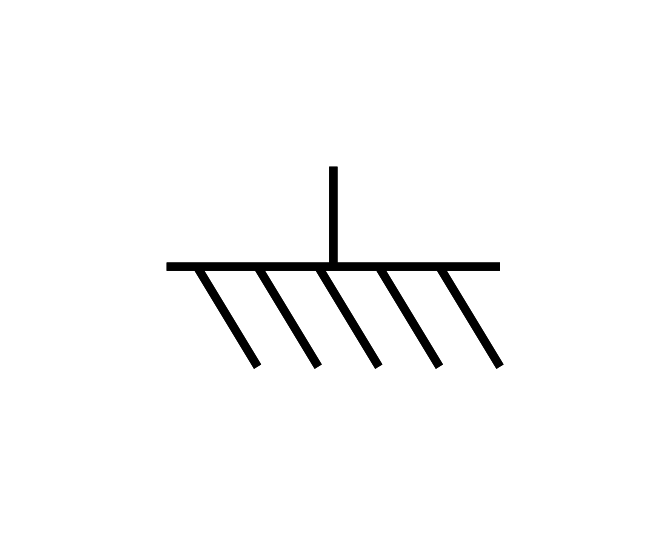
\includegraphics[width=0.75in]{generated_figures/bg_base_diagram.png}
\end{center}

\define{End Effector}{
    Drawn as follows, this represents a gripper or other end effector attached
    to the end of a robot link (or directly to the output of a joint). We
    generally do not consider the end effector to add a degree of freedom to the
    robot, as it does not take part in the overall kinematics.
}
\begin{center}
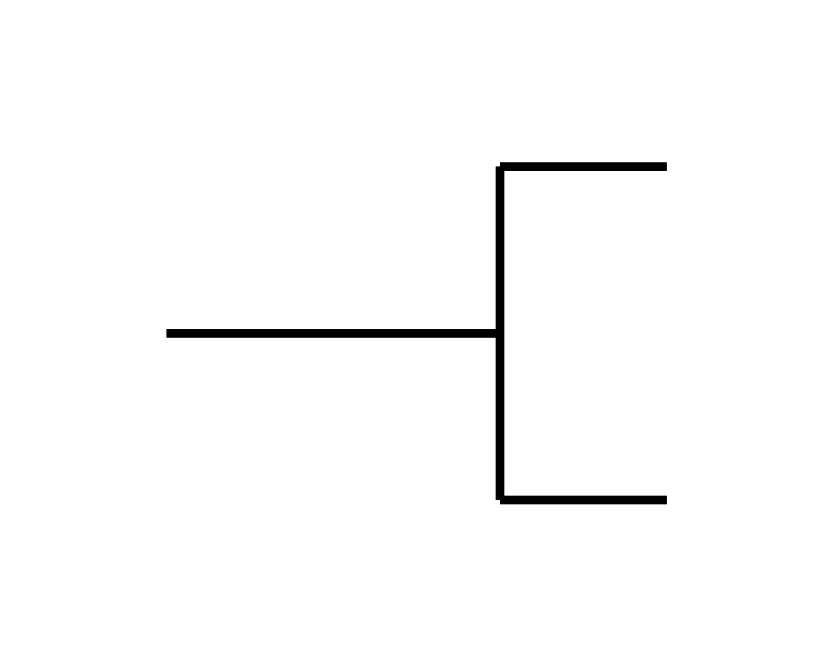
\includegraphics[width=0.75in]{generated_figures/bg_endeffector_diagram.png}
\end{center}

% directions

\define{Frame Conventions}{
    We define a \emph{base} frame as a coordinate frame at the point where the robot is fixed to
    the world, labeled \frame{0} (NOTE: in the OLI material, this frame is omitted).
    We also define a coordinate frame at the base of each link (the \emph{proximal}
    frame for that link).  Optionally, we can also define a frame at the \emph{end}
    of each link, where the next link is attached by a joint; this is the \emph{distal}
    frame. Note that this is also omitted in the OLI material, but is used in this
    assignment to help define the order of all intermediate transformations.
    The convention in this class will be that the $x$ axes of these frames points
    from the base to the end of the link. End effectors of planar robots will have a frame
    defined at the attachment point to the link, and the $x$ axes will point \emph{out} of the 
    gripper (i.e., this frame will usually match the distal frame of the connecting
    link). Positive angles of rotation will be counter-clockwise (from the $x$
    axis towards the $y$ axis). Below are several simple robots demonstrating
    these conventions.
}

\begin{center}
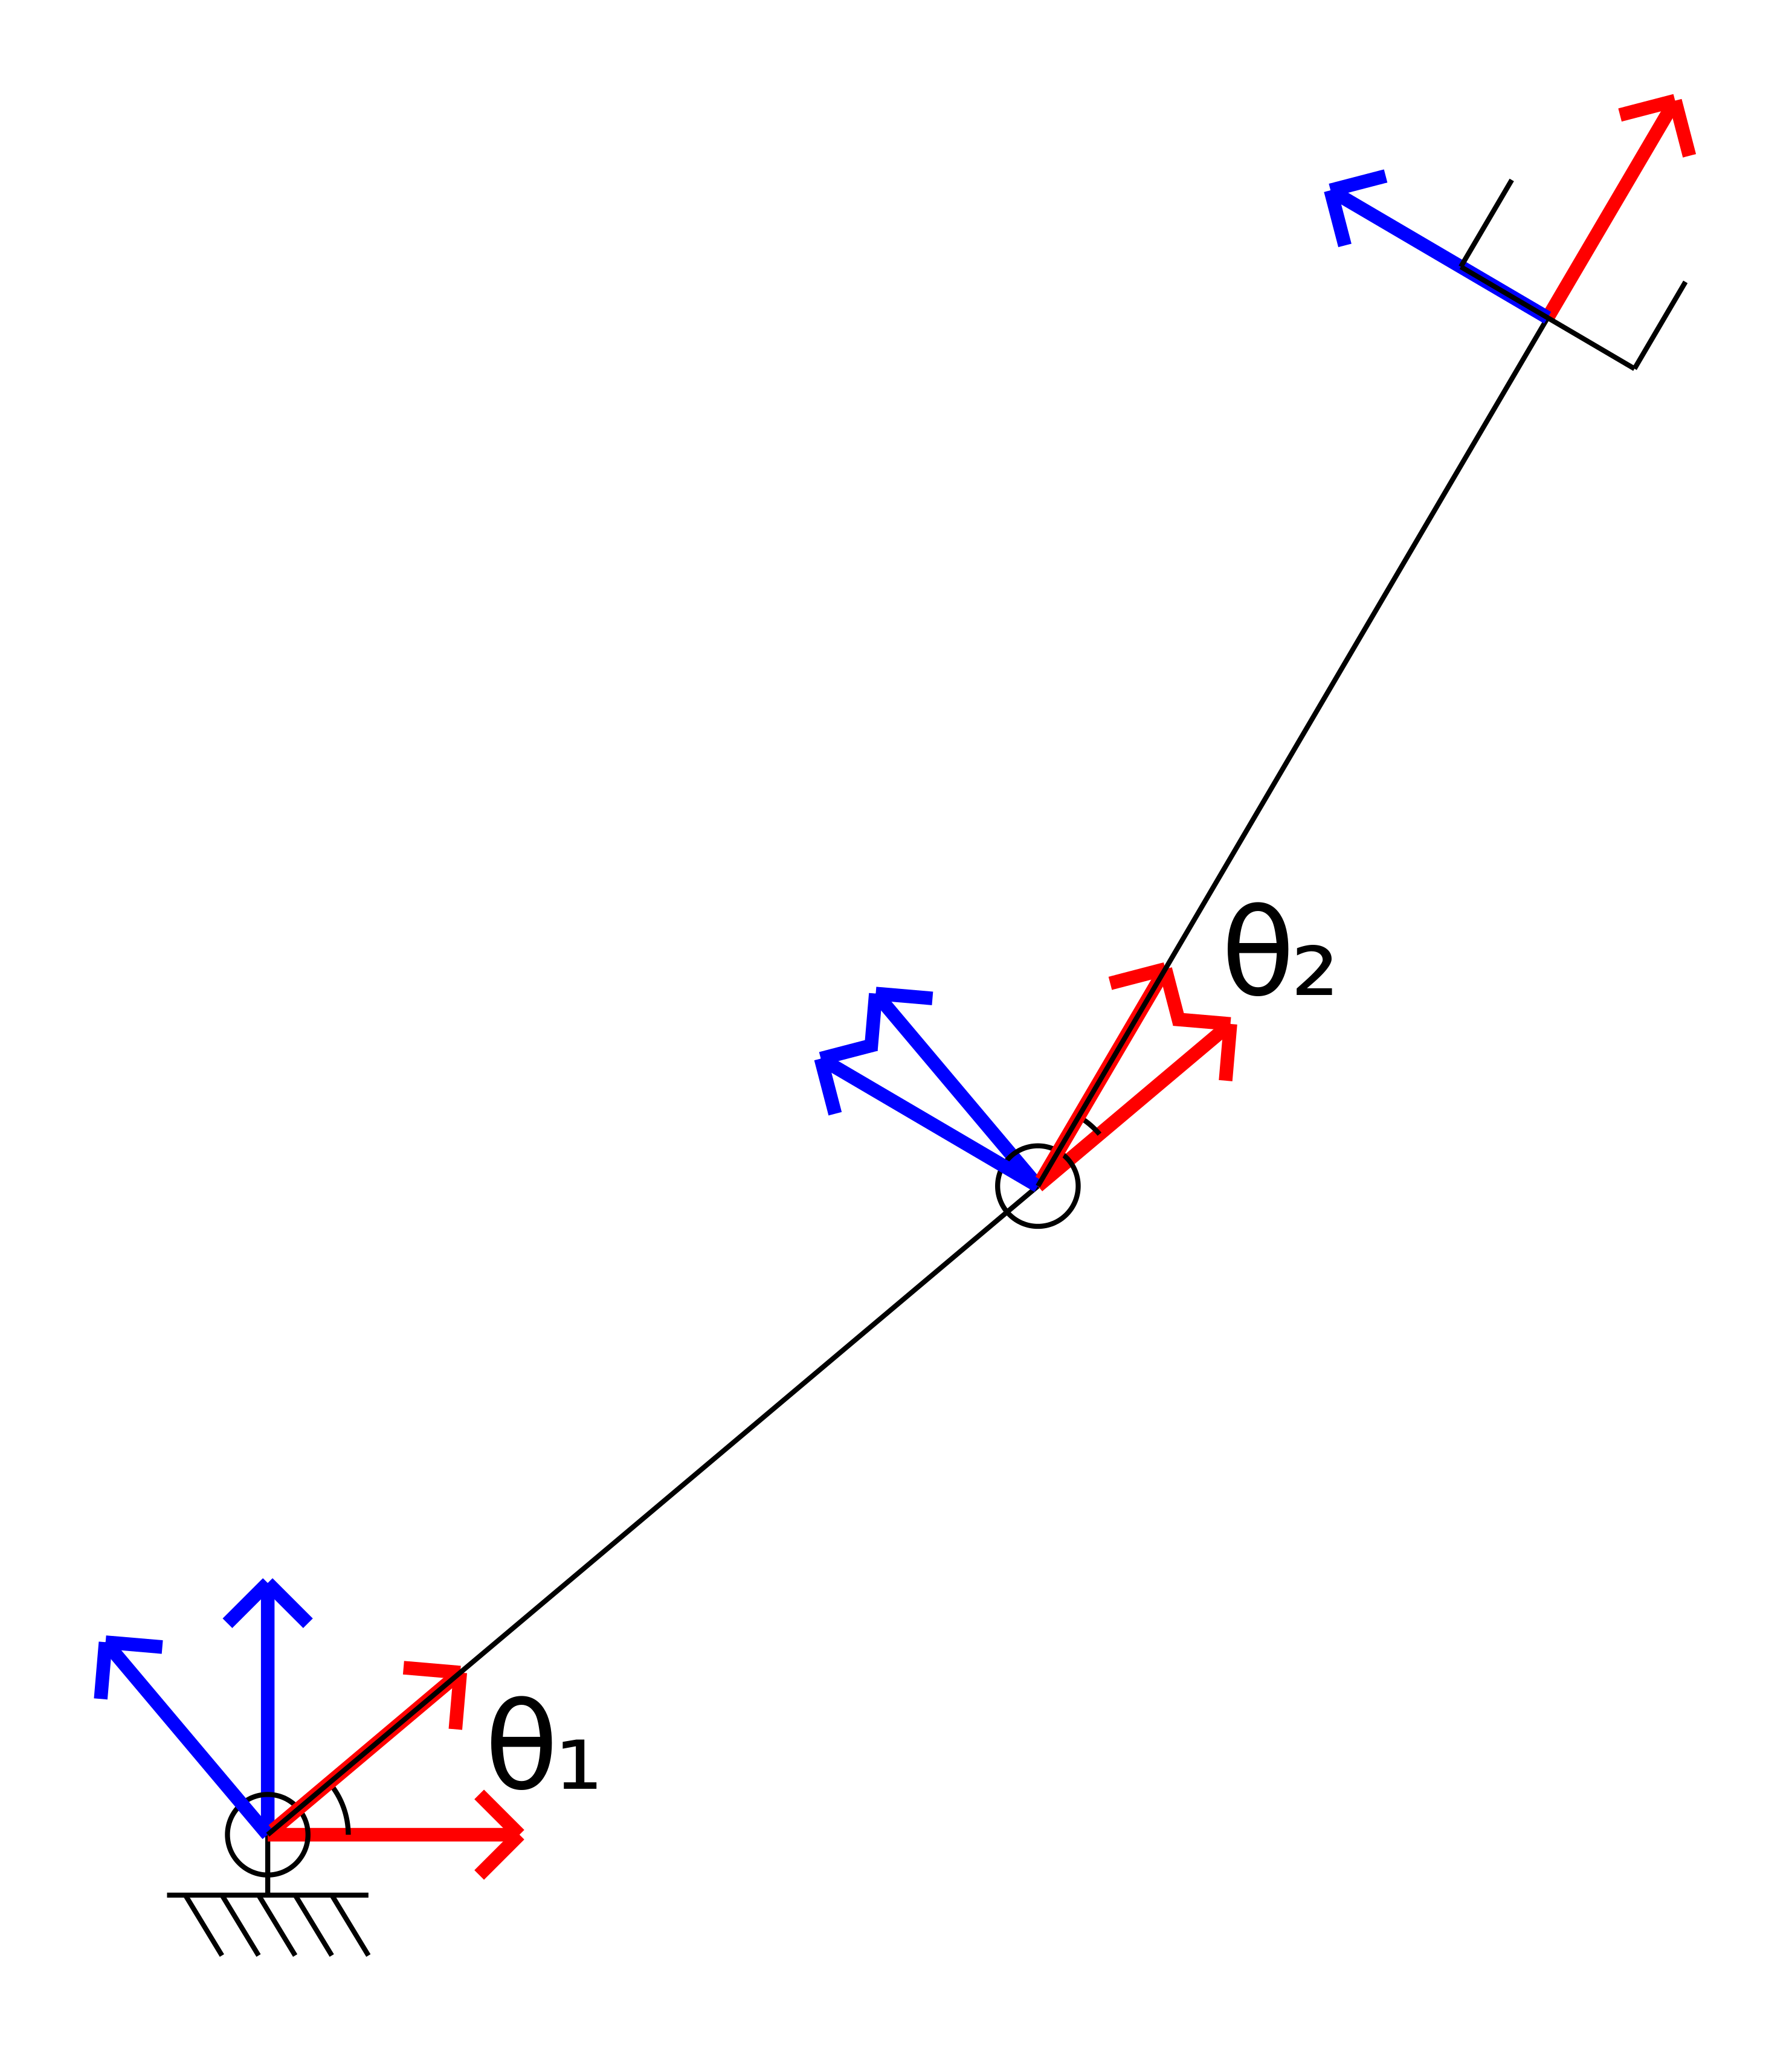
\includegraphics[scale=0.05]{generated_figures/bg_example_diagram_1.png}
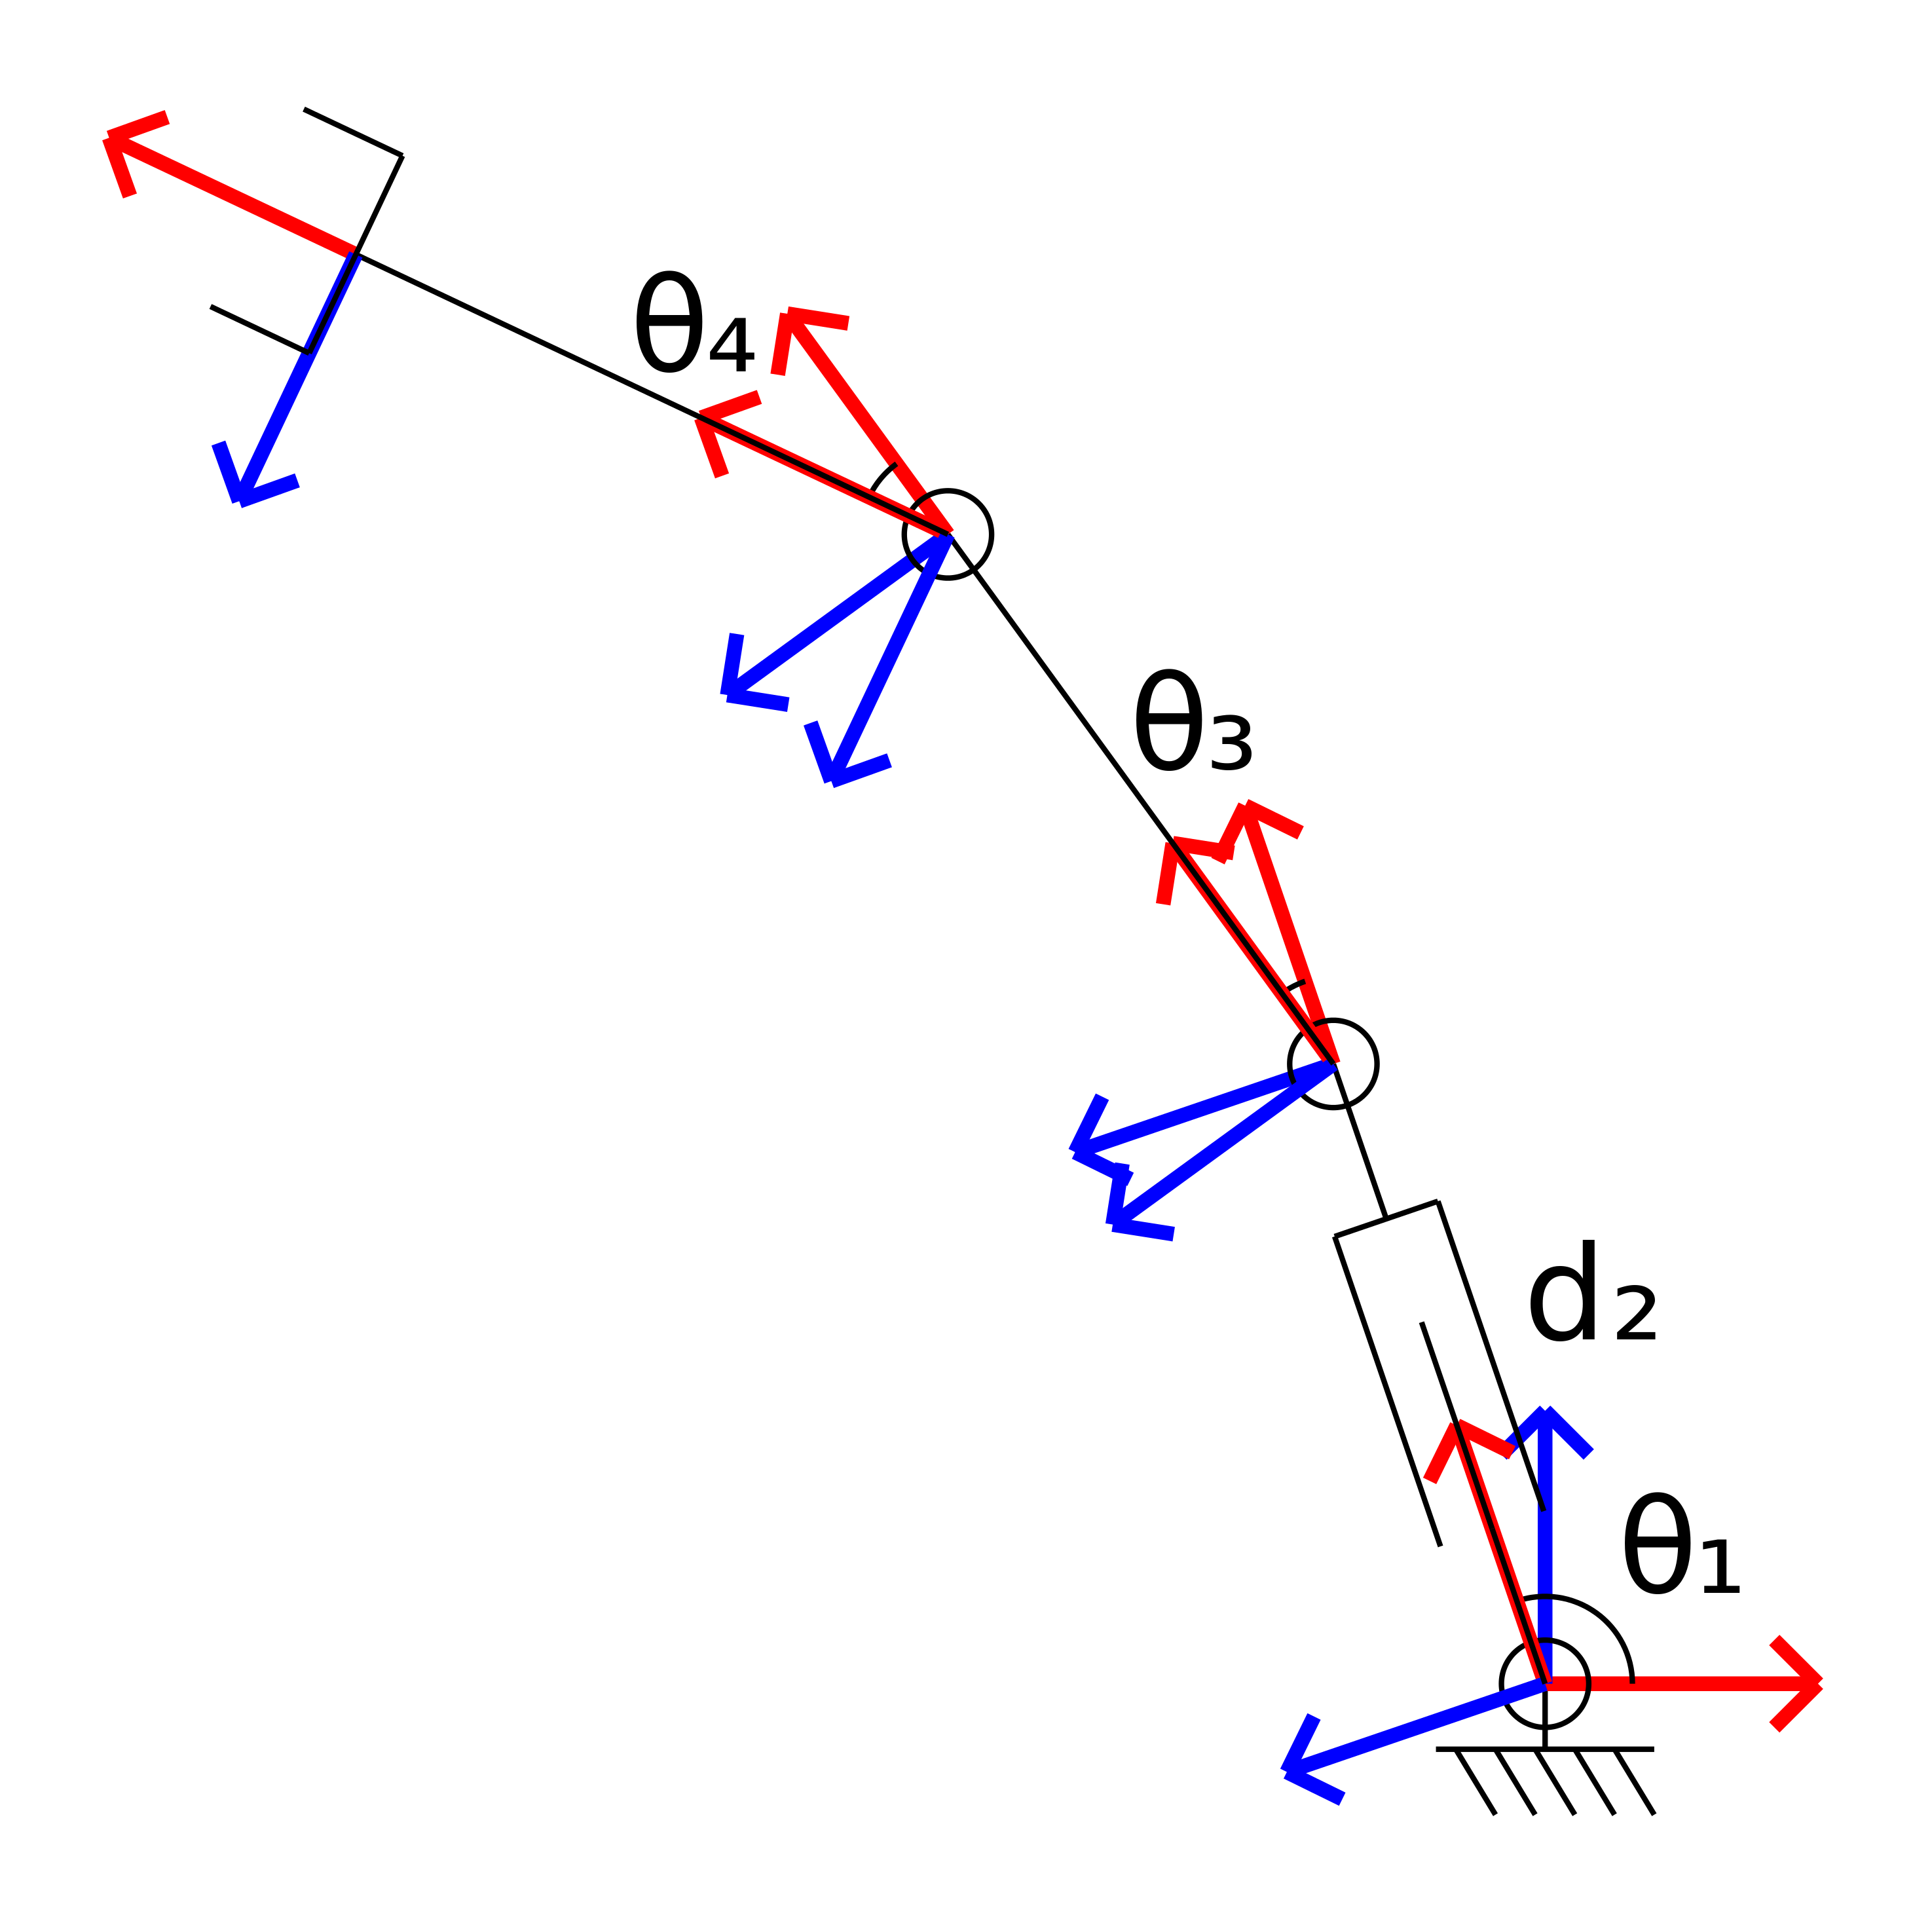
\includegraphics[scale=0.05]{generated_figures/bg_example_diagram_2.png}
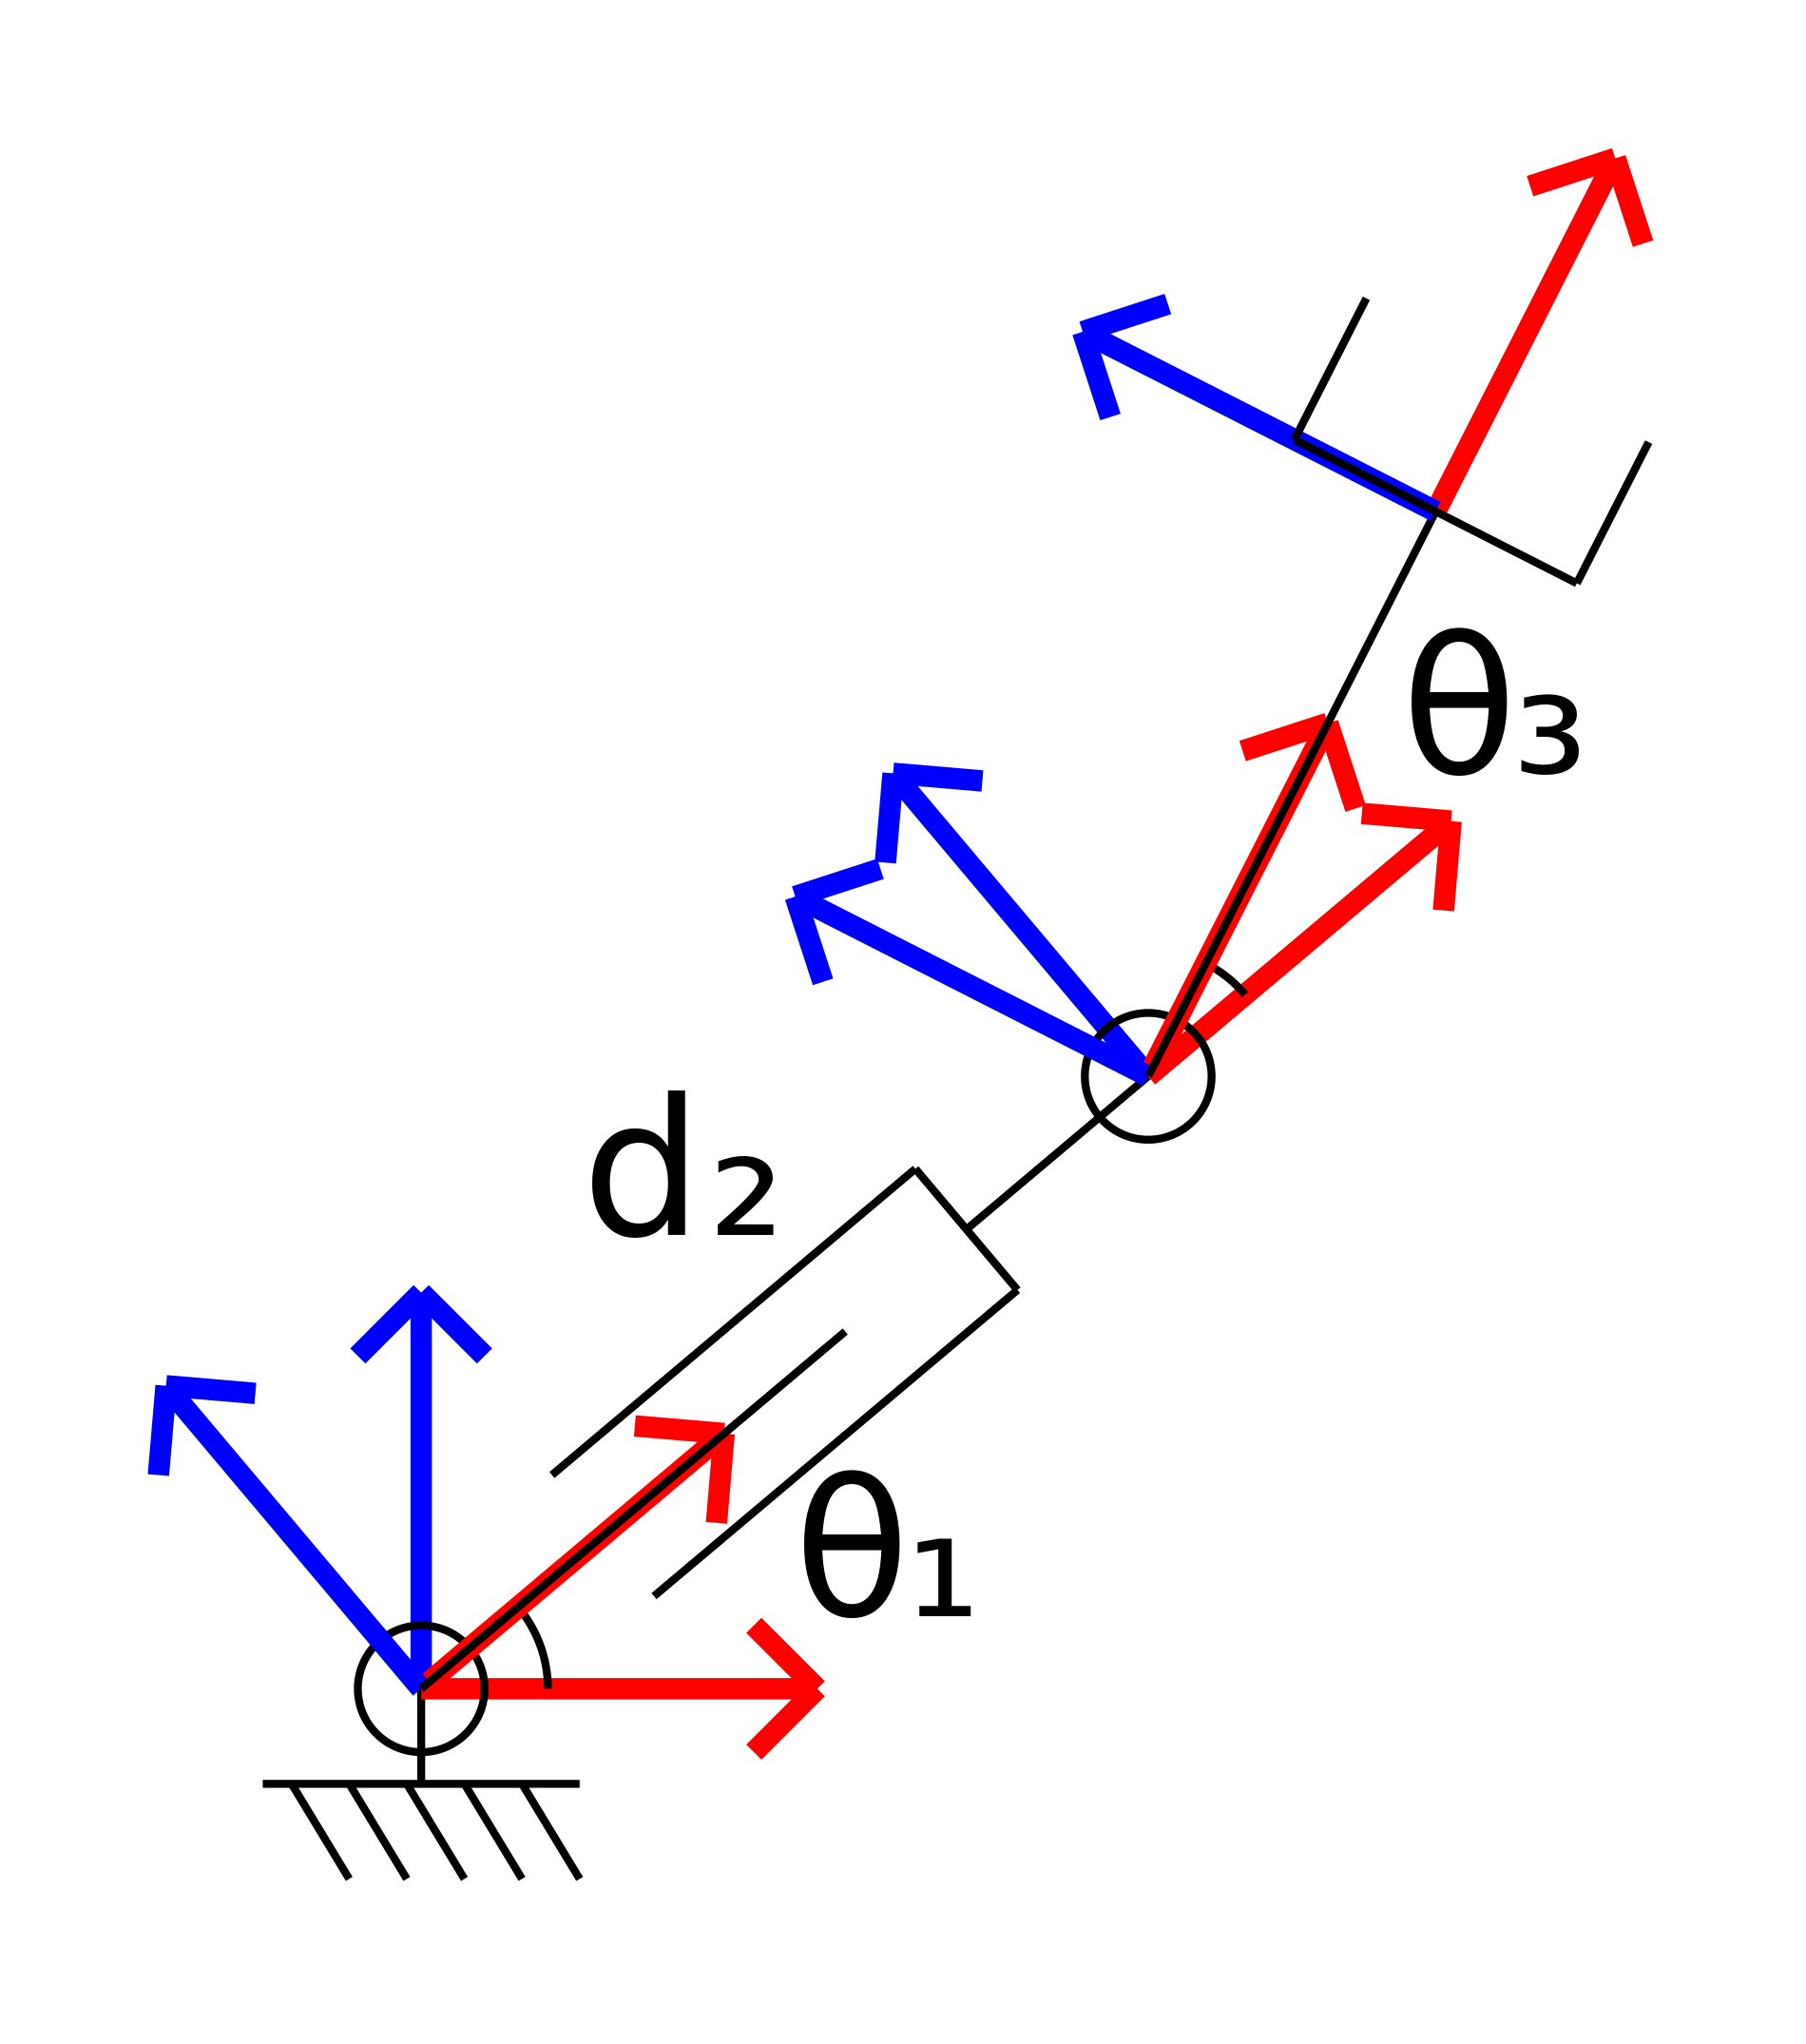
\includegraphics[scale=0.05]{generated_figures/bg_example_diagram_3.png}
\end{center}

\subsection{Degrees of Freedom}

In robot kinematics, a system's \emph{degrees of freedom}, or \emph{DOF}, is the number
of parameters needed to completely define a particular configuaration.  For example:

\begin{itemize}
    \item A point in two dimensions (i.e., $\RR^2$) has 2 DOF, since \smcolvec{x\\y} completely
        defines the point's configuration.

    \item A rigid body in the plane has 3 DOF, since \smcolvec{x\\y\\\theta}
        completely defines its position and orientation.

    \item An fixed-base n-joint kinematic chain in SE(2) has $n$ DOF, since $n$
    parameters for the joints completely define the robot's configuration.  If
    the robot isn't attached to the base frame, the base link can move freely
    (in $x$, $y$, and $\theta$), and the robot has $n + 3$ DOF.
\end{itemize}

\subsection{Rigid Motions / Transforms in Two Dimensions}

There are two basic types of motions/transformation we are concerned with:
rotations and translations. Rotations are represented with matrices, and
translations are represented by vectors.  These can be combined into compound
motions/transformations.

Rotations and translations are used for two different concepts.  The first is
the motion of a point or rigid body within a coordinate frame:

\begin{center}
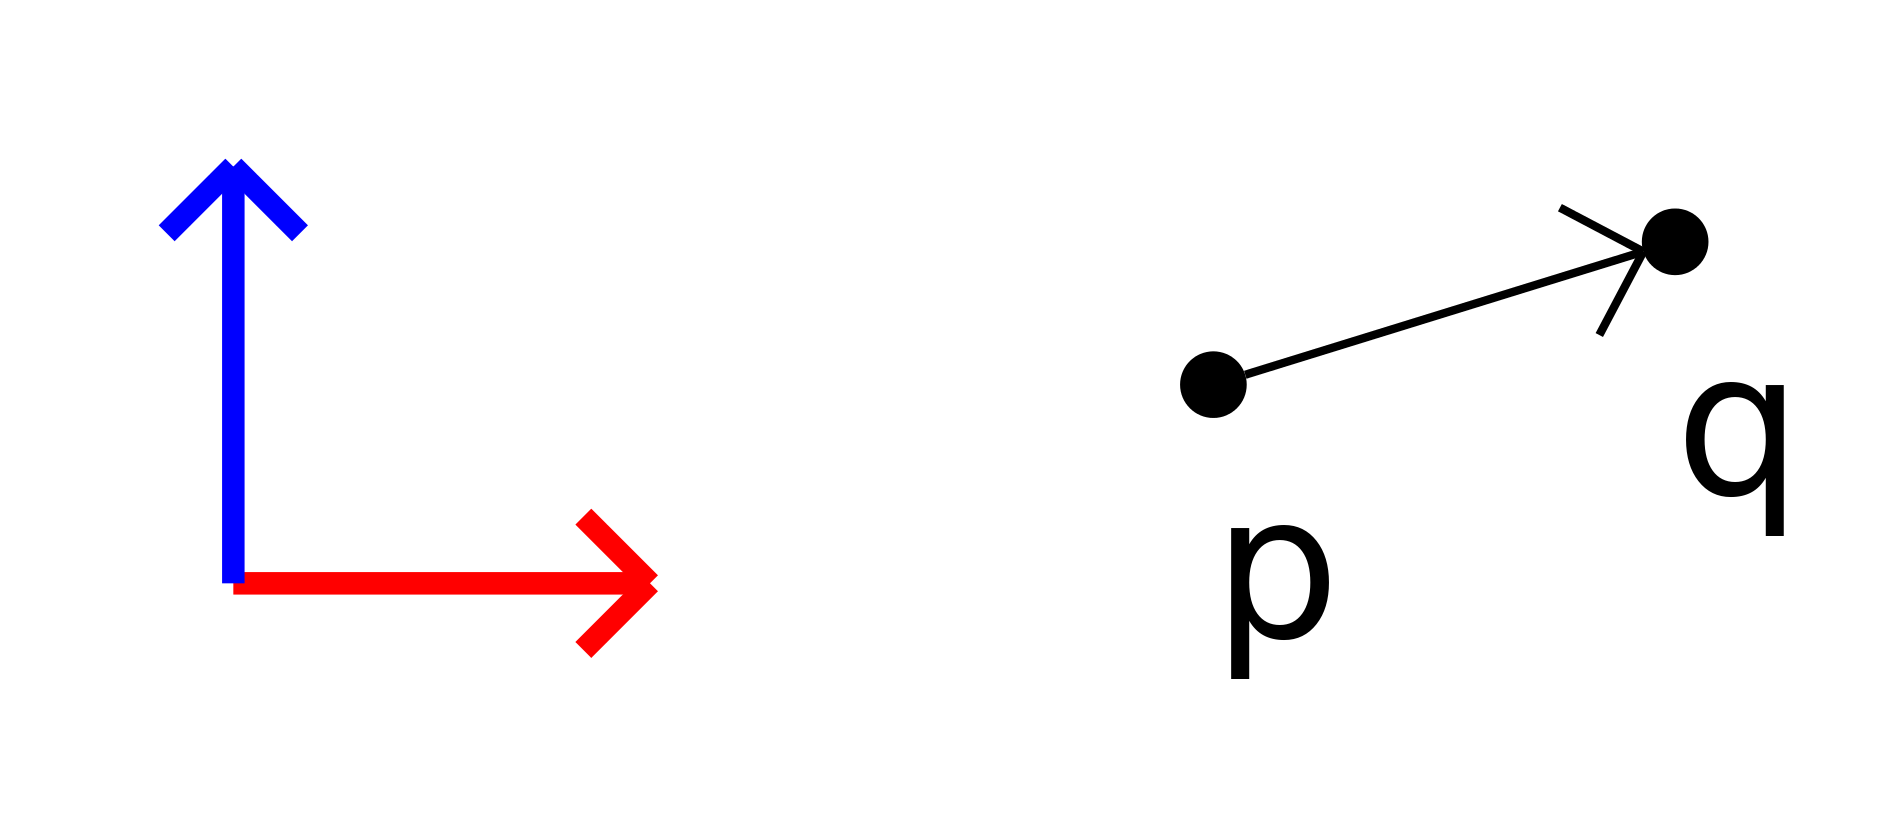
\includegraphics[scale=0.1]{generated_figures/bg_motion.png}
\end{center}

The second concept is a \emph{transform} between two coordinate frames. In
other words, if you have the coordinates of a point or vector in \frame{0}, what
are the coordinates of this same point or vector in \frame{1}:

\begin{center}
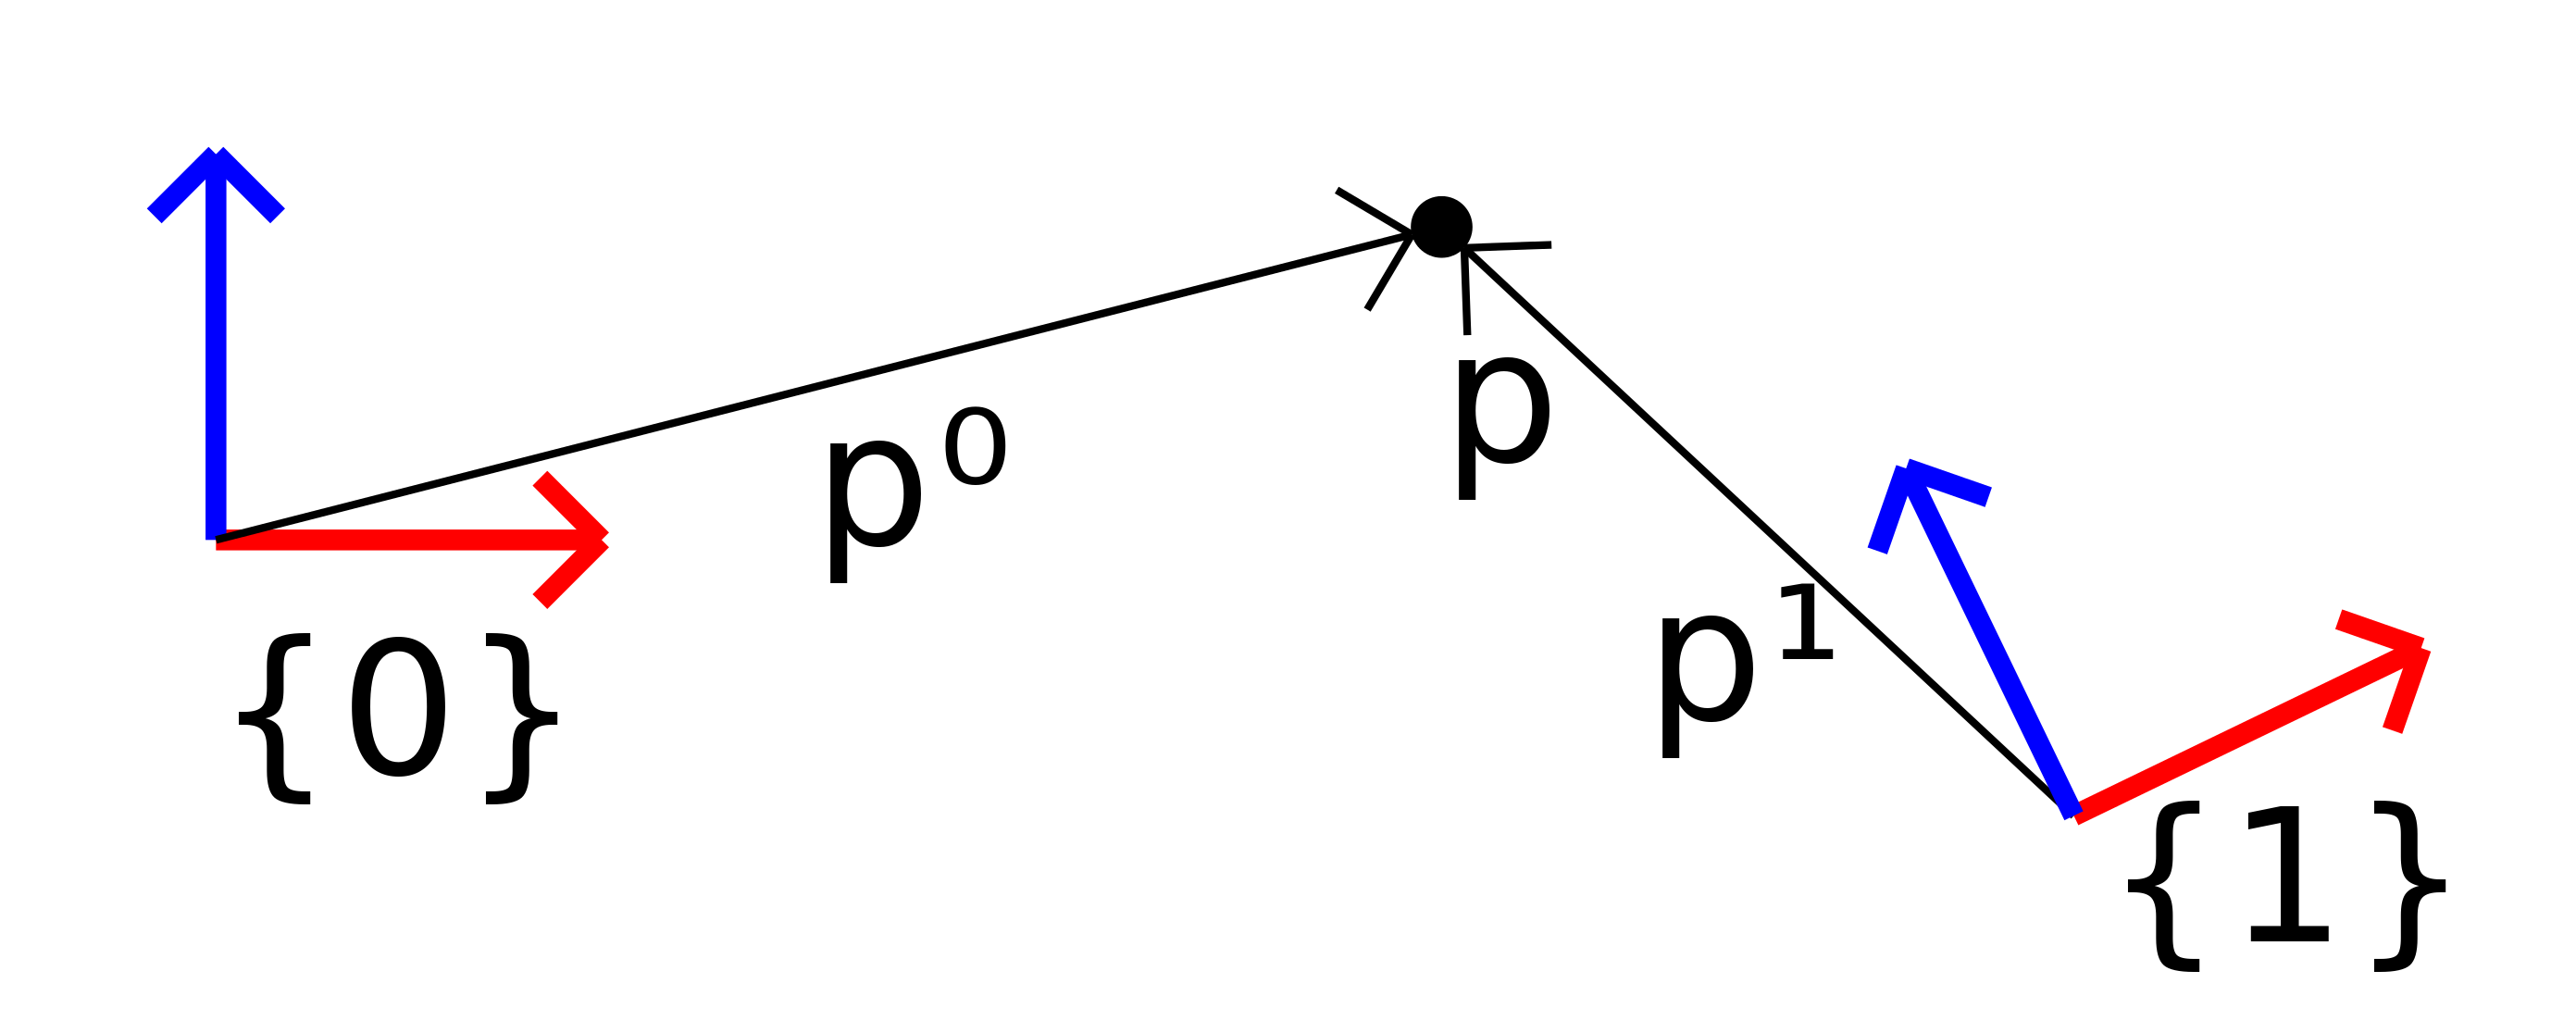
\includegraphics[scale=0.1]{generated_figures/bg_transform.png}
\end{center}

Notationally, transformations follow the convention of a superscript and a
subscript, to describe which frames are transformed between. A transform
$\transform{T}{b}{a}$ between two frames has several interpretations (notice
the order of the superscripts in each case).
\begin{itemize}
  \item The motion that moves \frame{a} to \frame{b}.
  \item \frame{b} as represented in \frame{a}.
  \item The transform that changes the representation of a point or vector from
    \frame{b} to \frame{a}.
\end{itemize}

\vspace{0.2in}
Note that the motion between two frames is the opposite of the transform that
changes point representation between these frames. This is something which can
often lead to errors! A good rule of thumb is that the top number always represents what
frame this motion/transform is represented in.  Here, the transform is in
the frame of reference \frame{a}. Below, we explicitly consider translations, rotations, and combined motions.

\subsubsection{Translation}

% Drawing of frames i and j, where j is offset by \smcolvec{\Delta x\\\Delta y}
\begin{center}
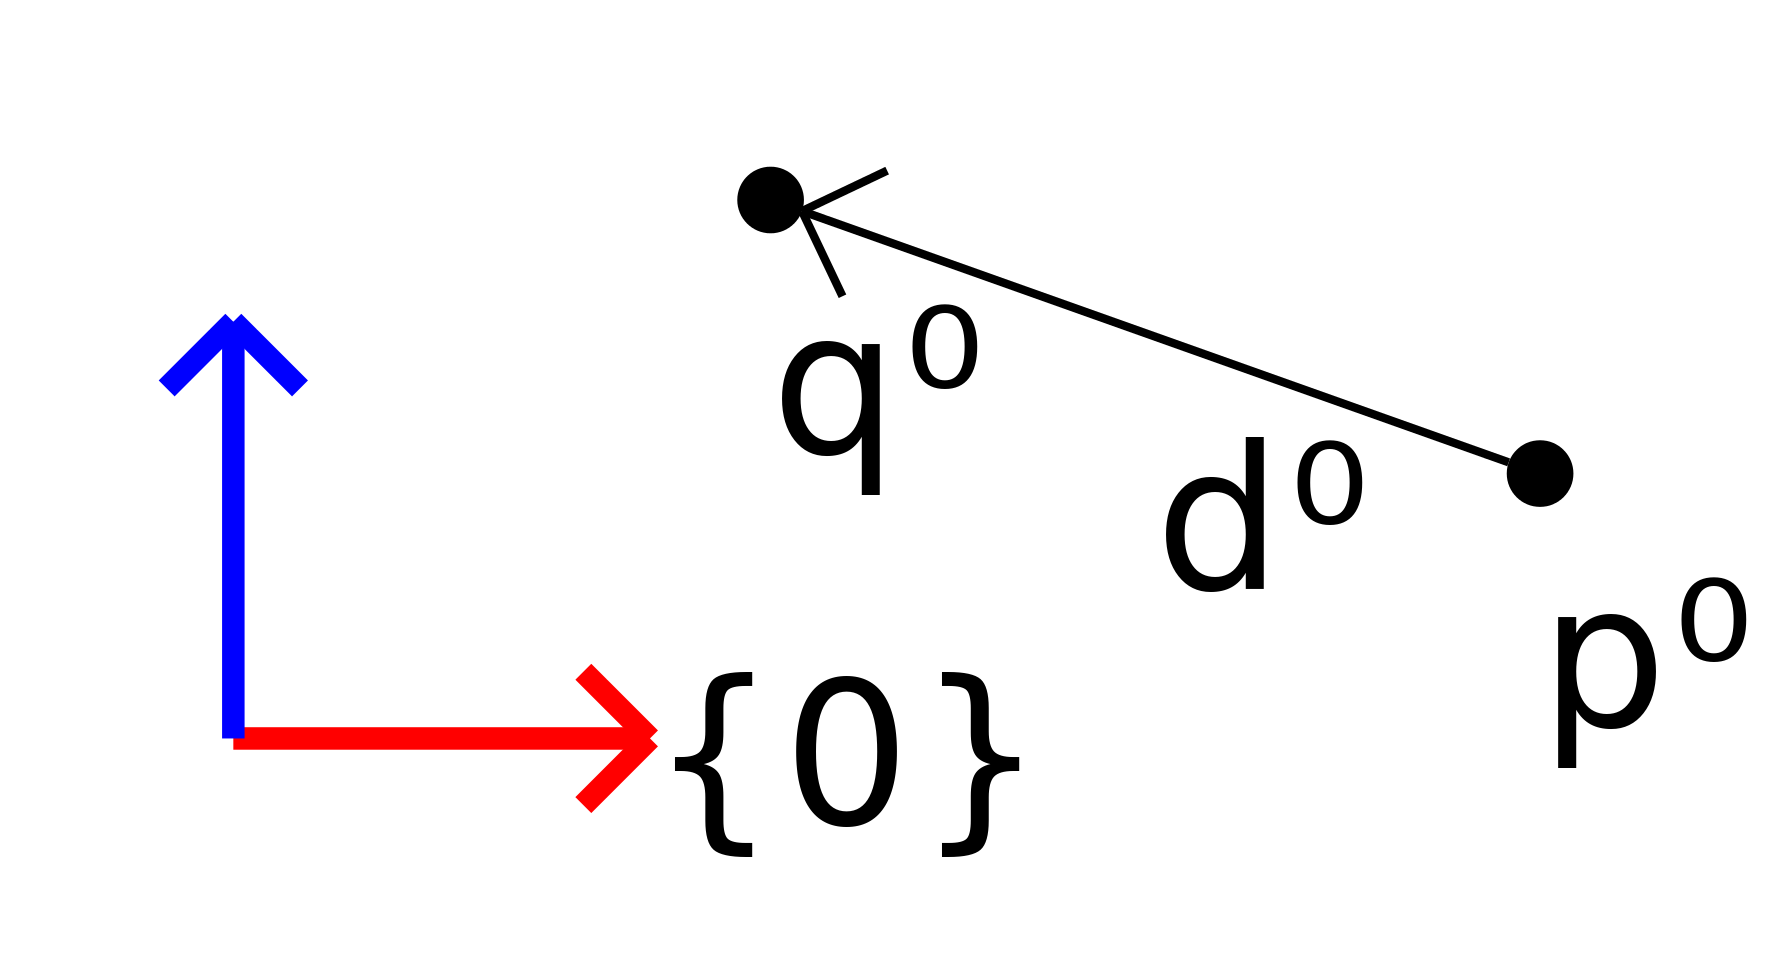
\includegraphics[scale=0.09]{generated_figures/bg_translation_motion.png}
\hspace{0.5in}
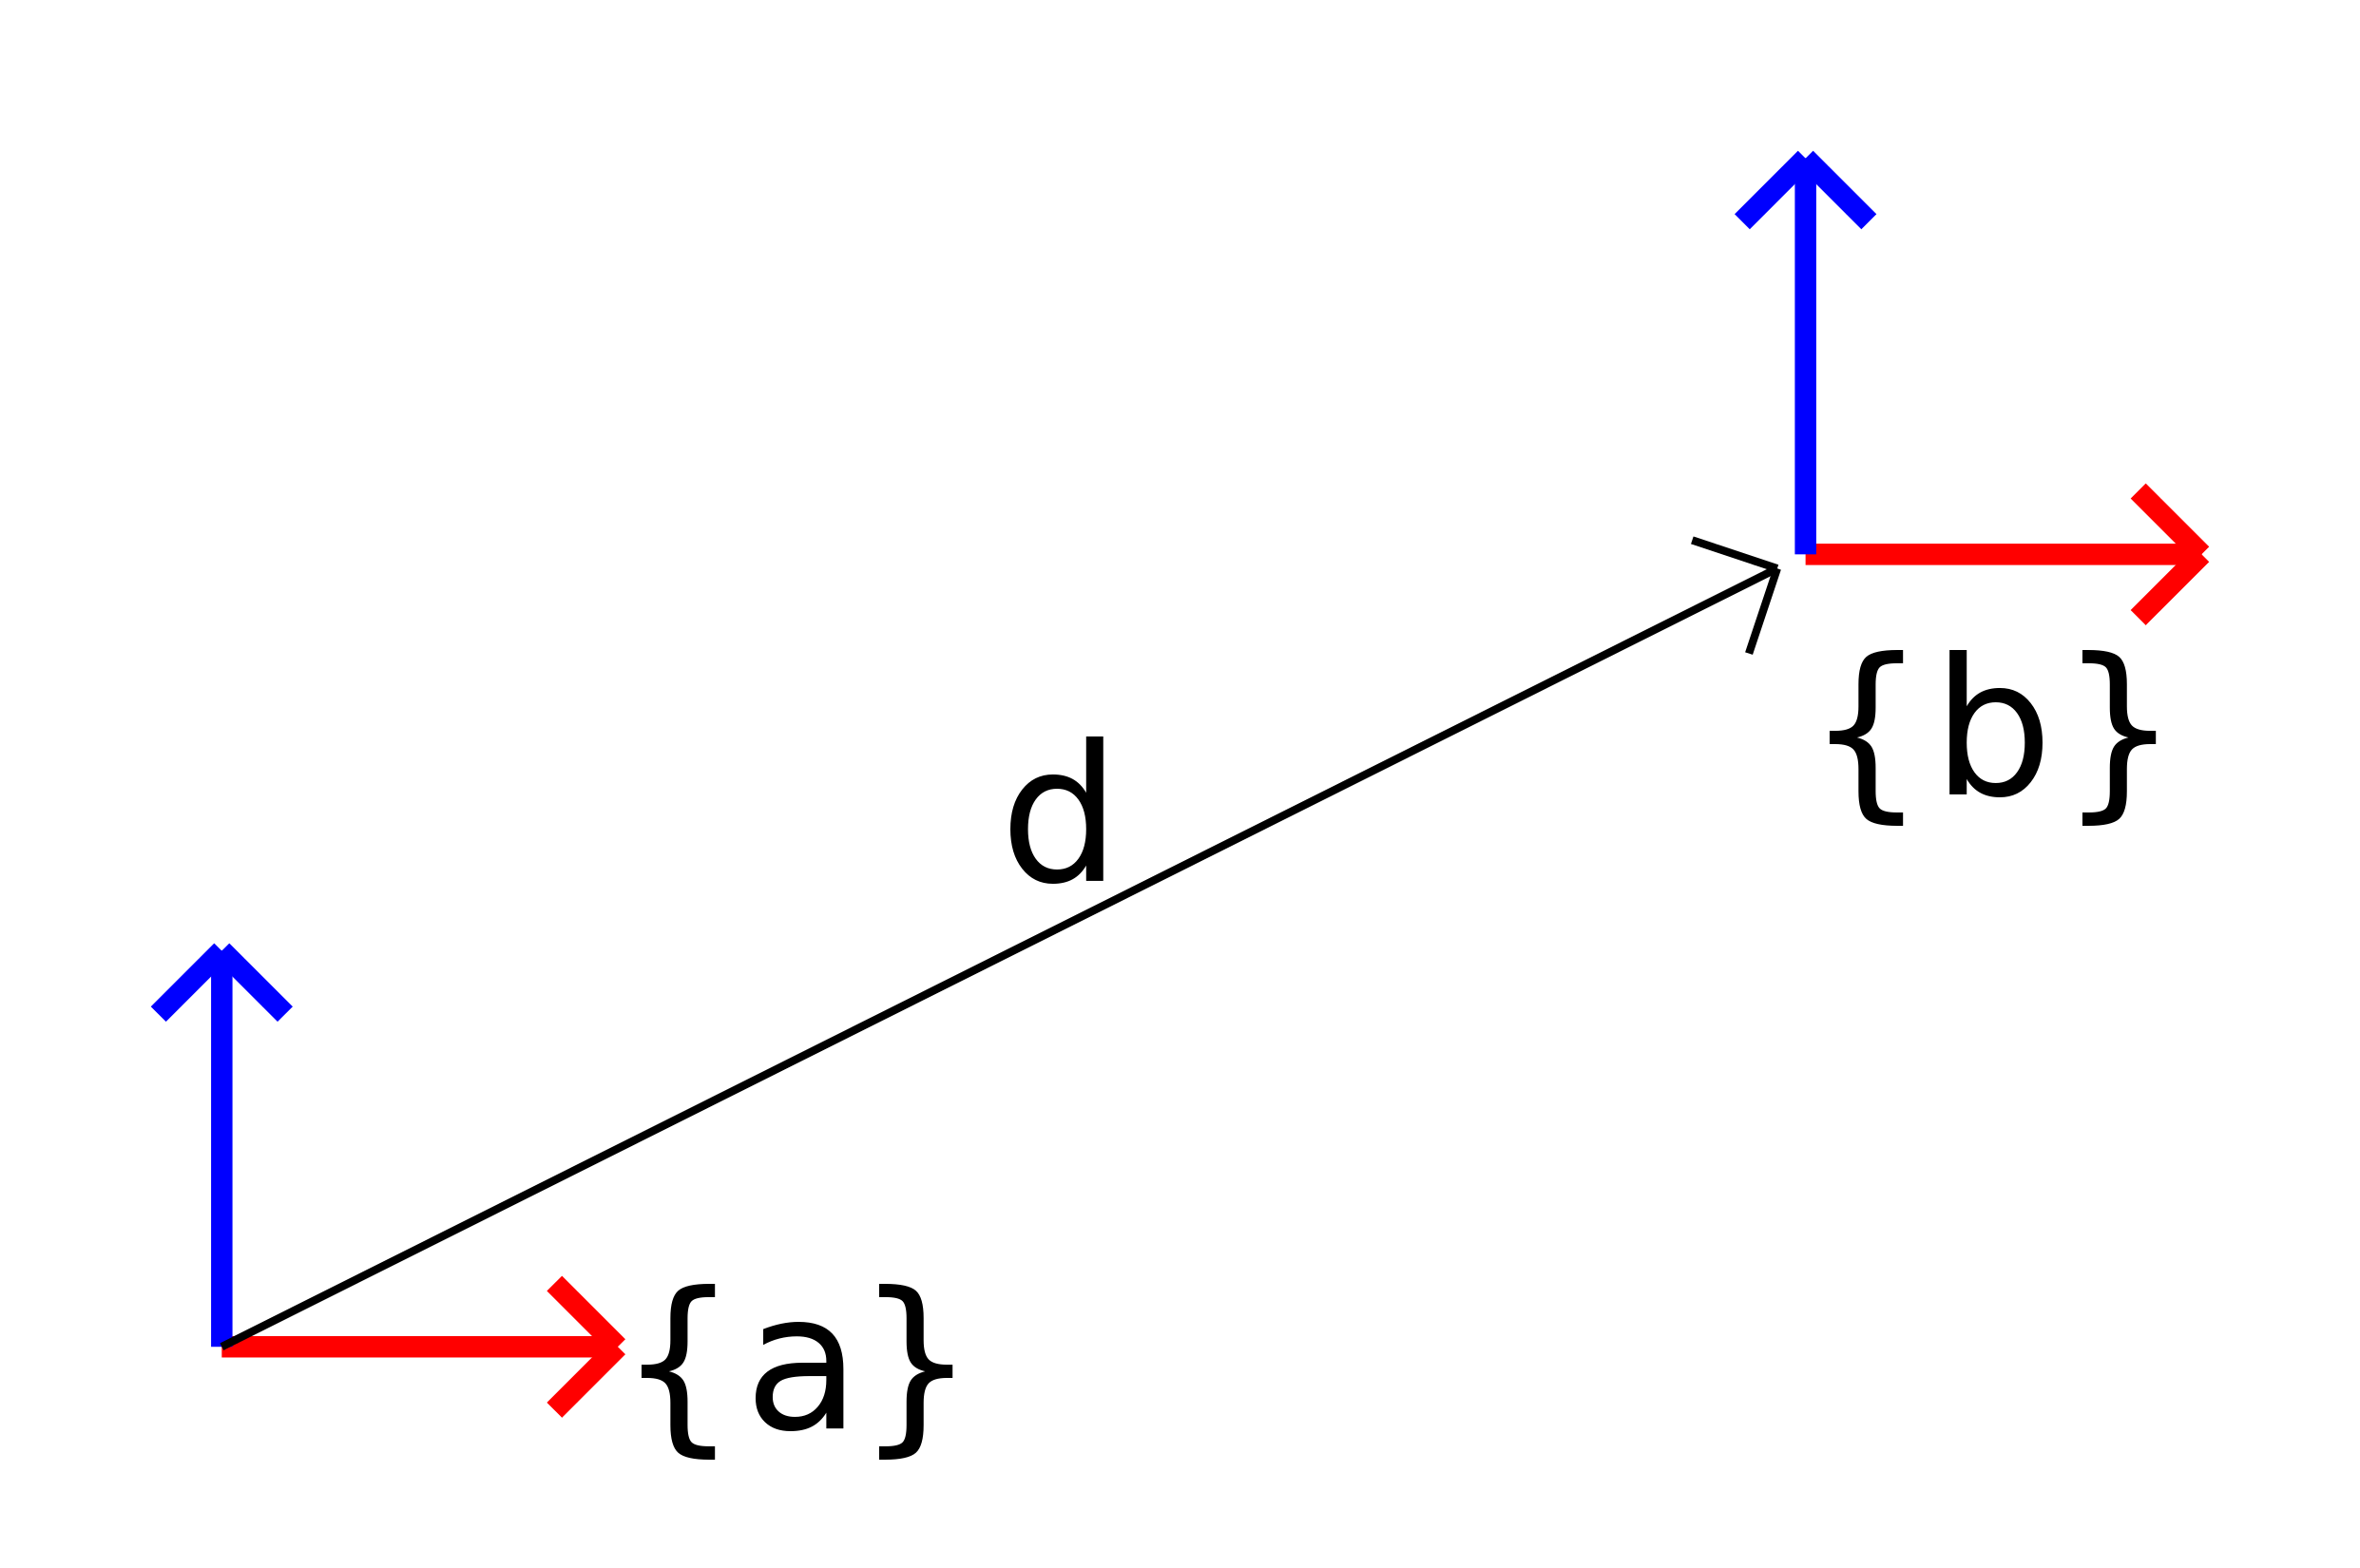
\includegraphics[scale=0.09]{generated_figures/bg_translation.png}
\end{center}

A translation $\t{}{} = \smcolvec{\Delta x\\\Delta y}$ expresses a change in
position of a point or rigid body, or a position offset between coordinate
frames. In terms of rigid motions, translating a point is the geometric addition of two
positions; above left, $\transform{q}{}{0} = \p{0} + \t{}{0}$. This is the motion
that moves $\p{}$ to $\transform{q}{}{}$ in \frame{0}.

For transformations, \t{b}{a} is the offset from \frame{a} to \frame{b} (above
right, $\t{}{} = \t{b}{a} = \smcolvec{4\\2}$). In other words, \t{b}{a} is:
\begin{itemize}
  \item The motion that moves (the origin) of \frame{a} to the origin of
    \frame{b}.
  \item The representation of \frame{b} in \frame{a} (e.g., the coordinates of
    the origin of \frame{b} in \frame{a}).
  \item The transform that changes the representation of a point $p$ from
    \frame{b} to \frame{a}: $\p{a} = \t{b}{a} + \p{b}$.
\end{itemize}

\subsubsection{Rotation}

\begin{center}
% Drawing of rotation of vector by \theta
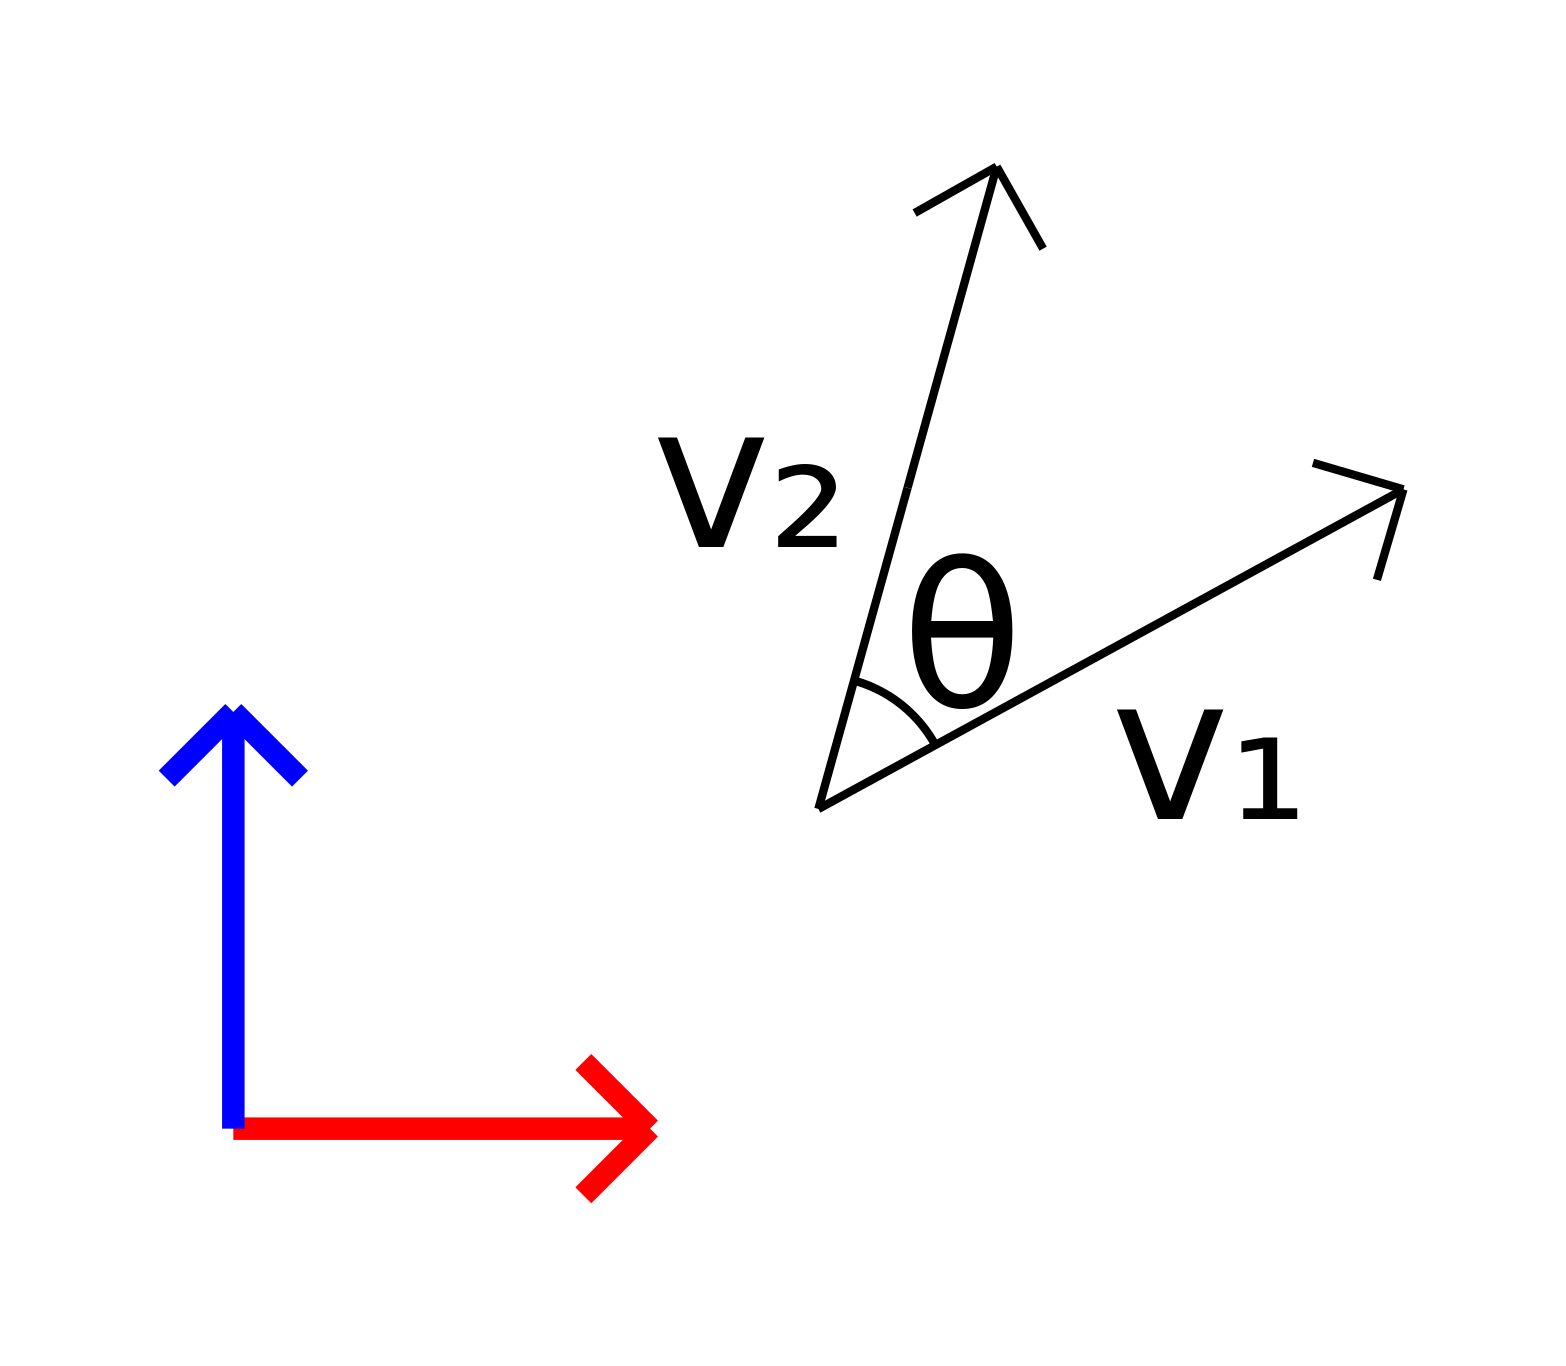
\includegraphics[scale=0.1]{generated_figures/bg_rotate_vec.png}
\hspace{1in}
% Drawing of frames i and j, where j is offset by \th
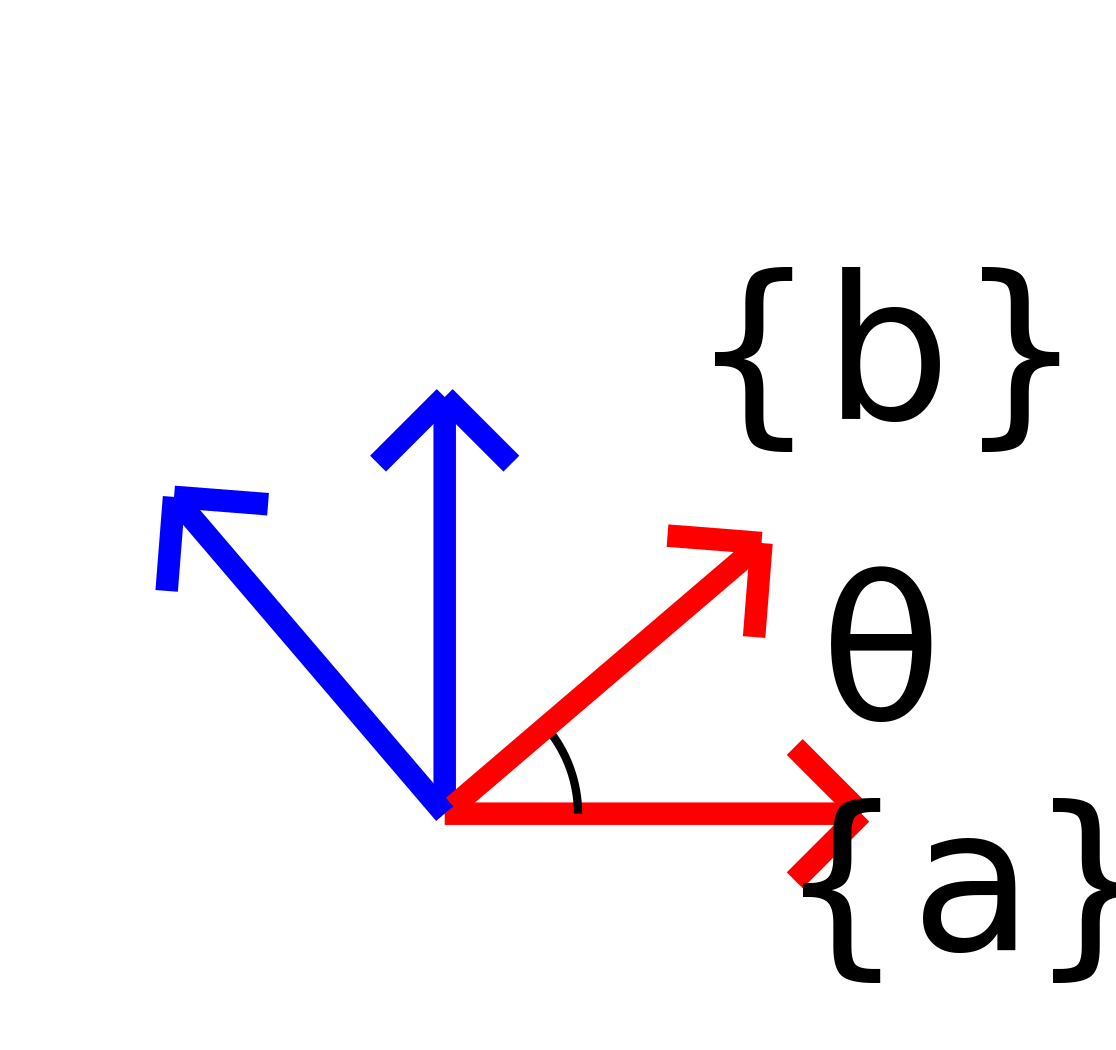
\includegraphics[scale=0.1]{generated_figures/bg_rotation.png}
\end{center}

A \emph{rotation matrix} \R{}{} represents rigid body rotations or rotational
offsets between coordinate frames.  In 2 dimensions, the rotation matrix
corresponding to a rotation of $\theta$ is
$$
\R{}{}(\theta) = \colvec{\cos(\theta)&-\sin(\theta)\\\sin(\theta)&\cos(\theta)}
$$

For rigid motions, this is the rotation of a body or vector by $\theta$; above
left, the vector $v_2 = \R{}{}(\theta) v_1$.

For transformations, \R{b}{a} is the rotation from \frame{a} to \frame{b} (above
right, $\R{b}{a} = \R{}{}(\theta)$). $\R{b}{a}$ can be described as:
\begin{itemize}
  \item The motion that rotates \frame{a} to \frame{b}.
  \item The representation of \frame{b} in \frame{a}; $\R{b}{a}$ can be found by
    expressing the axes of \frame{b} in \frame{a} as column vectors.
  \item The rotation that changes the representation of a vector $v$ from
    \frame{b} to \frame{a}: $\v{a} = \R{b}{a} \v{b}$.
\end{itemize}

\vspace{0.2in}
Furthermore, as shown in lecture, for any
rotation matrix \mat{R}, \inv{\mat{R}} = \trans{\mat{R}}.

\subsubsection{Compound Motions: Homogeneous Transforms}

Any rigid motion/transform between two frames can be expressed by combining a
single rotation and translation.  A \emph{homogeneous transform} is a single
matrix which allows us to express this combined rotation and translation:

$$
\H{b}{a} = \colvec{\R{b}{a}&\t{b}{a}\\0~0&1}
$$

As with previous notation, \H{b}{a} is a motion from \frame{a} to \frame{b}, or
equivalently the transform that changes the coordinates of points from \frame{b}
to \frame{a}.

% [ Drawing of frames i and j, where j is rotated by theta and offset by some
\begin{center}
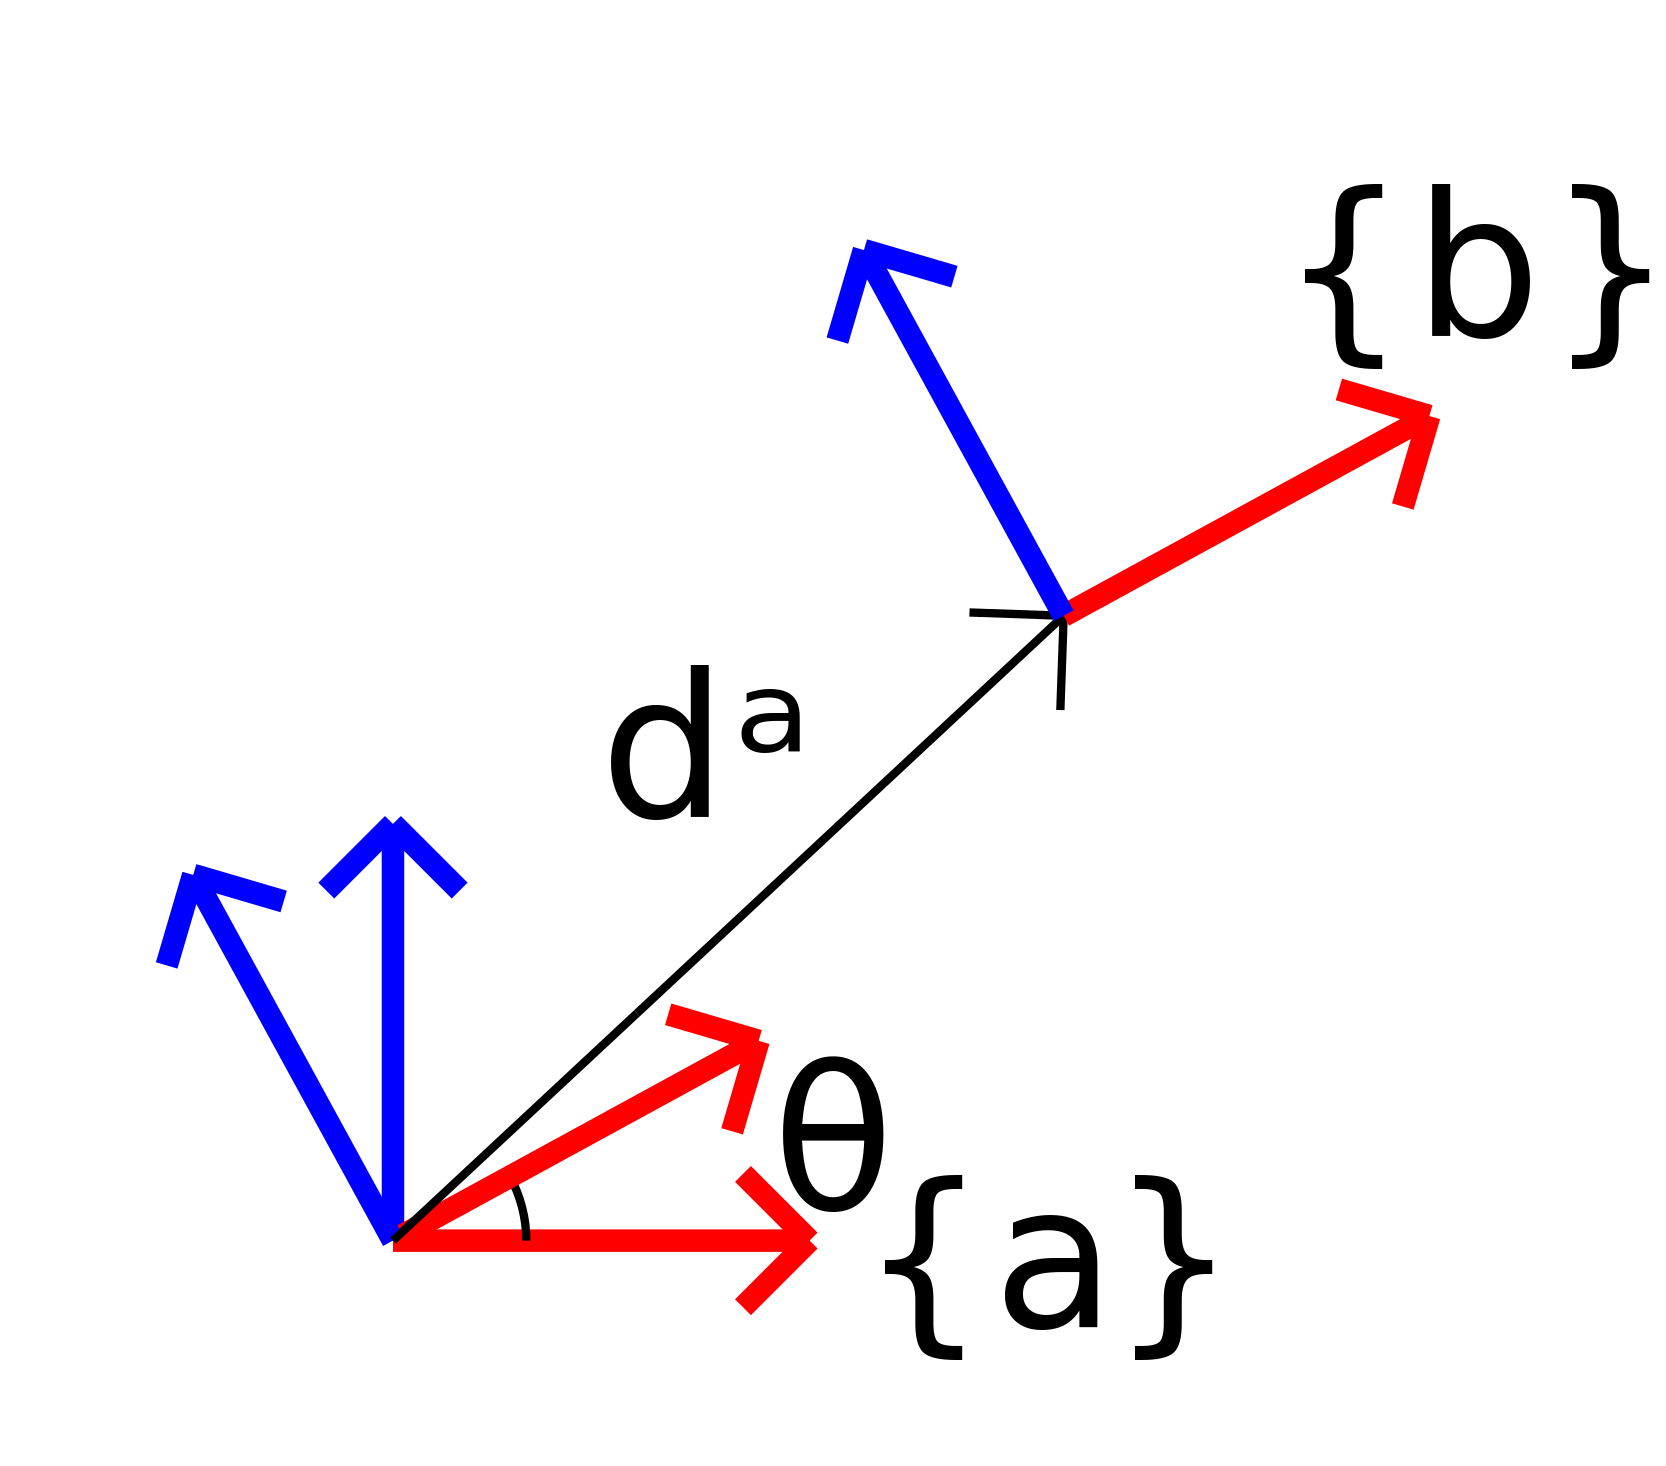
\includegraphics[scale=0.1]{generated_figures/bg_homo_r_then_t.png}
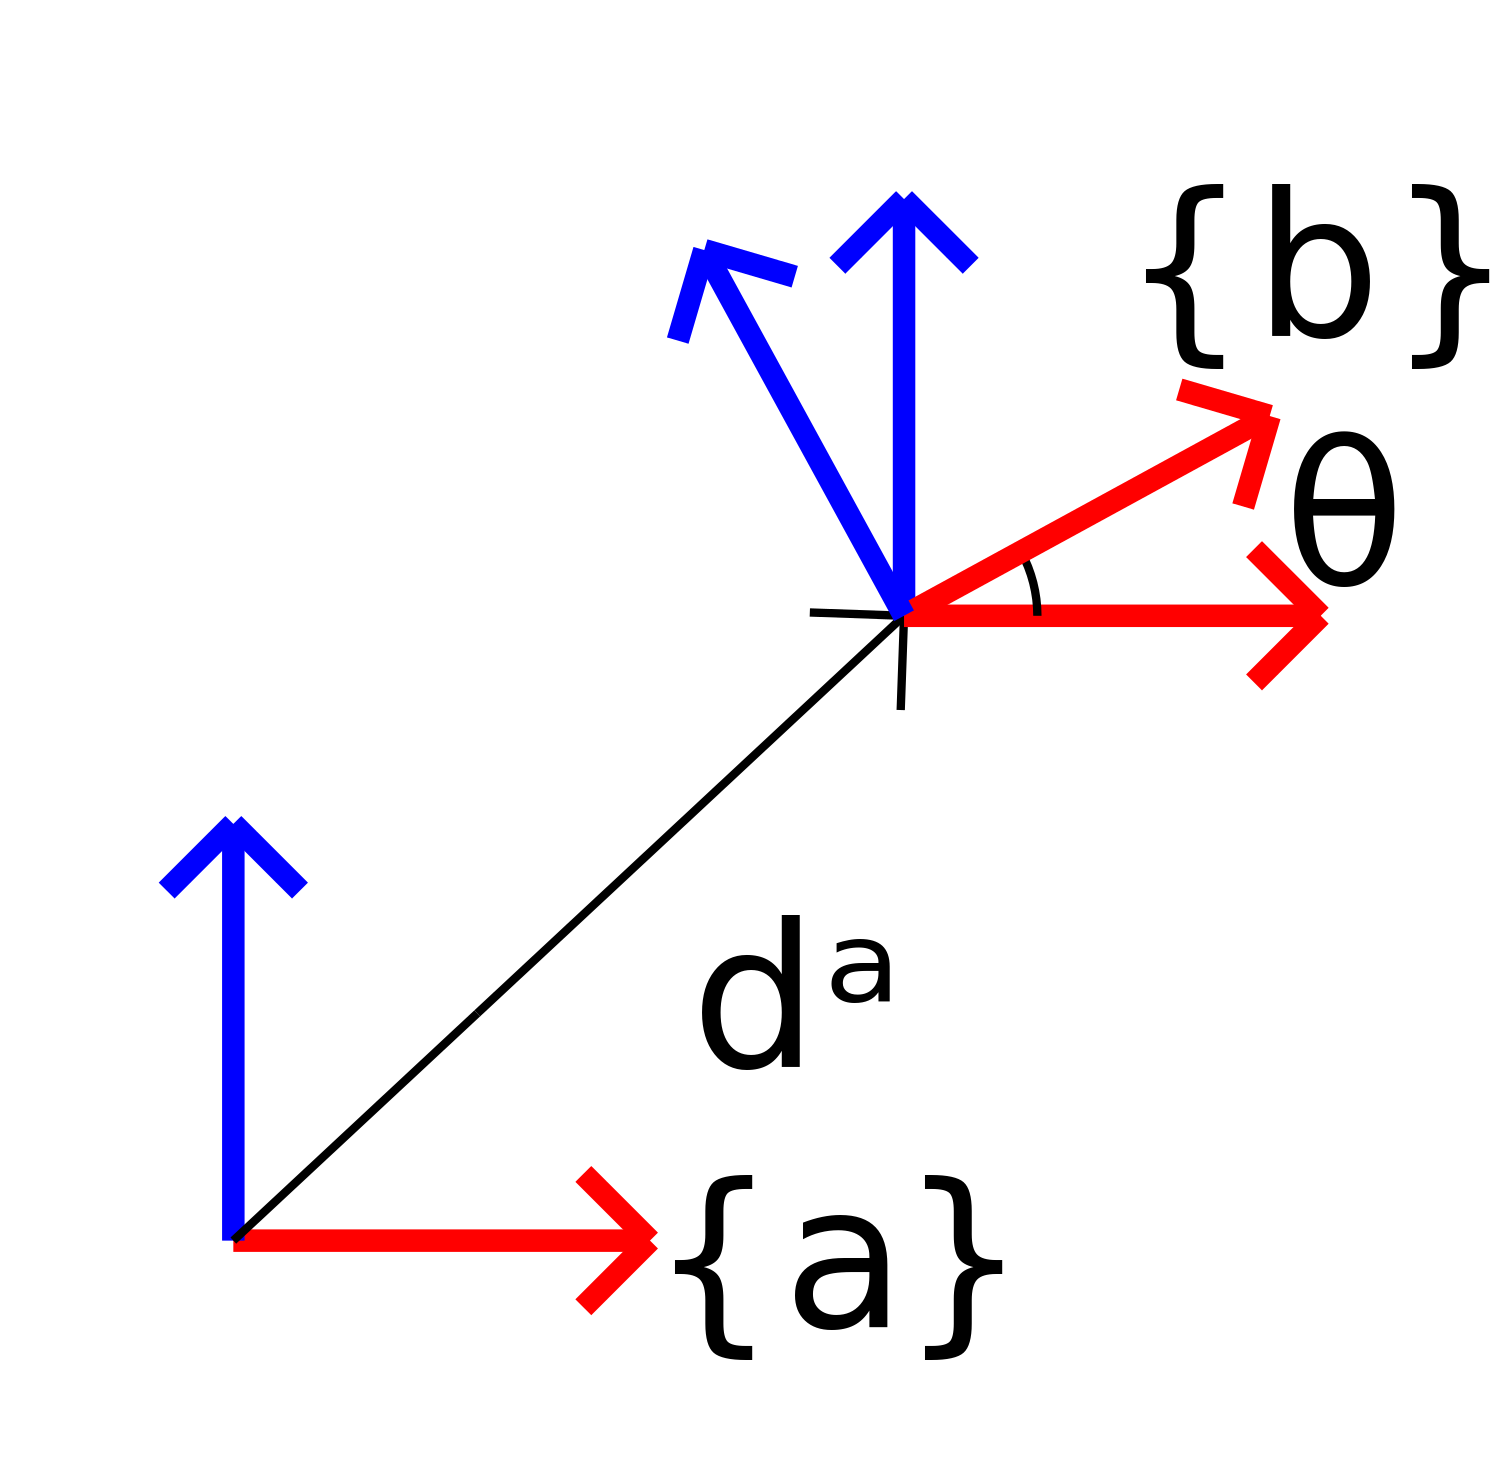
\includegraphics[scale=0.1]{generated_figures/bg_homo_t_then_r.png}
\end{center}

An important point here is that the \emph{order} and \emph{frame of reference}
which you apply the rotation and transforms here matter. The following two
descriptions are equivalent (and describe \H{b}{a}):
\begin{itemize}
\item First apply the rotation relative to \frame{a}, and then apply the
translation relative to \frame{a} (see above left).
\item First apply the translation relative to \frame{a} and then apply to
rotation relative to the \emph{new} frame resulting from this translation (see
above right).
\end{itemize}

Note that the other two potential descriptions - rotation then translation in
the new frame, or translation then rotation in \frame{a} - are both equivalent
but \textbf{do not describe \H{b}{a}}.

\subsubsection{Points, Vectors, and Homogeneous Transforms}

When using Homogeneous Transforms to operate on points and vectors, we must add
an extra coordinate to these values. Points are padded with a 1, so $\p{i} =
\smcolvec{p_x\\p_y}$ is now \smcolvec{p_x\\p_y\\1}, whereas vectors are padded with a 0,
so $\v{i} = \smcolvec{v_x\\v_y}$ is now \smcolvec{v_x\\v_y\\0}. This allows the
matrix dimensions to match when multiplying by such transforms.

If $\H{}{0}$ describes a motion in \frame{0}, then the point $\transform{q}{}{0}$
resulting from this motion starting at point $\p{0}$ is:

\begin{eqnarray*}
\transform{q}{}{0} &=& \H{}{0} \colvec{\p{0}\\1} \\
&=& \colvec{\R{}{0}&\t{}{0}\\0~0&1} \colvec{\p{0}\\1} \\
&=& \R{}{0} \p{0} + \t{}{0} \\
\end{eqnarray*}

Note that the $1$ we added to the bottom of the point results in the addition of
$\t{}{0}$; because free vectors have a $0$ added, they are only affected by the
rotation portion of \H{}{0}.

Using $\H{b}{a}$ as a transformation between coordinate representations of
points/vectors, we have

$$
\smcolvec{\p{a}\\1} = \H{b}{a} \smcolvec{\p{b}\\1} \text{and} \smcolvec{\v{a}\\0} = \H{b}{a} \smcolvec{\v{b}\\0}.
$$

\subsubsection{Inverting \H{b}{a}}
The inverse of \H{b}{a} is \H{a}{b}, representing the opposite motion, or a
reverse transform between the two frames.

To invert \H{b}{a}, we could perform the matrix inversion manually,
but there is a faster method using the properties of \H{b}{a}. First,
recall that \p{a} = \R{b}{a} \p{b} + \t{b}{a}.  Solving for \p{b}, we can see
that \p{b} = \trans{\R{b}{a}}\p{a} - \trans{\R{b}{a}}\t{b}{a}.  Therefore, given
\R{b}{a} and \t{b}{a}, \R{a}{b} = \trans{\R{b}{a}} and \t{a}{b} =
-\trans{\R{b}{a}}\t{b}{a}.  This finally gives us that

$$
\inv{\H{b}{a}} = \H{a}{b} = \smcolvec{\trans{\R{b}{a}}&(-\trans{\R{b}{a}}\t{b}{a})\\\trans{\vec{0}}&1}
$$

Inspection can show that this holds true for \v{a} and \v{b} as well.

\subsubsection{Composing Transforms}

Homogeneous transforms are composable. For example:
$$
\H{2}{0} = \H{1}{0} \H{2}{1}
$$

Note that in expressions like \p{1} = \H{0}{1}\p{0}, the superscripts ``cancel''
out, which gives you a quick check for your systems of equations.  However, note
that multiplication of transformations is \textbf{not} commutative and this
cancellation only works diagonally one way: $\H{2}{0} \ne \H{2}{1} \H{1}{0}$.
Using superscripts for the frame of points and vectors will help enforce this
consistency.

Furthermore, \inv{\H{i}{j}} = \H{j}{i}, so if we are given \H{1}{0}, \H{1}{2},
and \H{3}{2}, we can find \H{3}{0} = \H{1}{0}\inv{\H{1}{2}}\H{3}{2}.

\subsection{Forward Kinematics}

Forward kinematics is the idea of taking a robot's input parameters (joint
angles, link lengths, etc.) and finding the position of the end effector. We can do
this by writing homogeneous transforms that use the input parameters as
variables in order to find the final end effector position.  In effect, we want
to define frames at each link and joint and describe their differences in terms
of the robot parameters.

Let us consider the single link R arm of length $d$.
% DRAWING OF ARM
\begin{center}
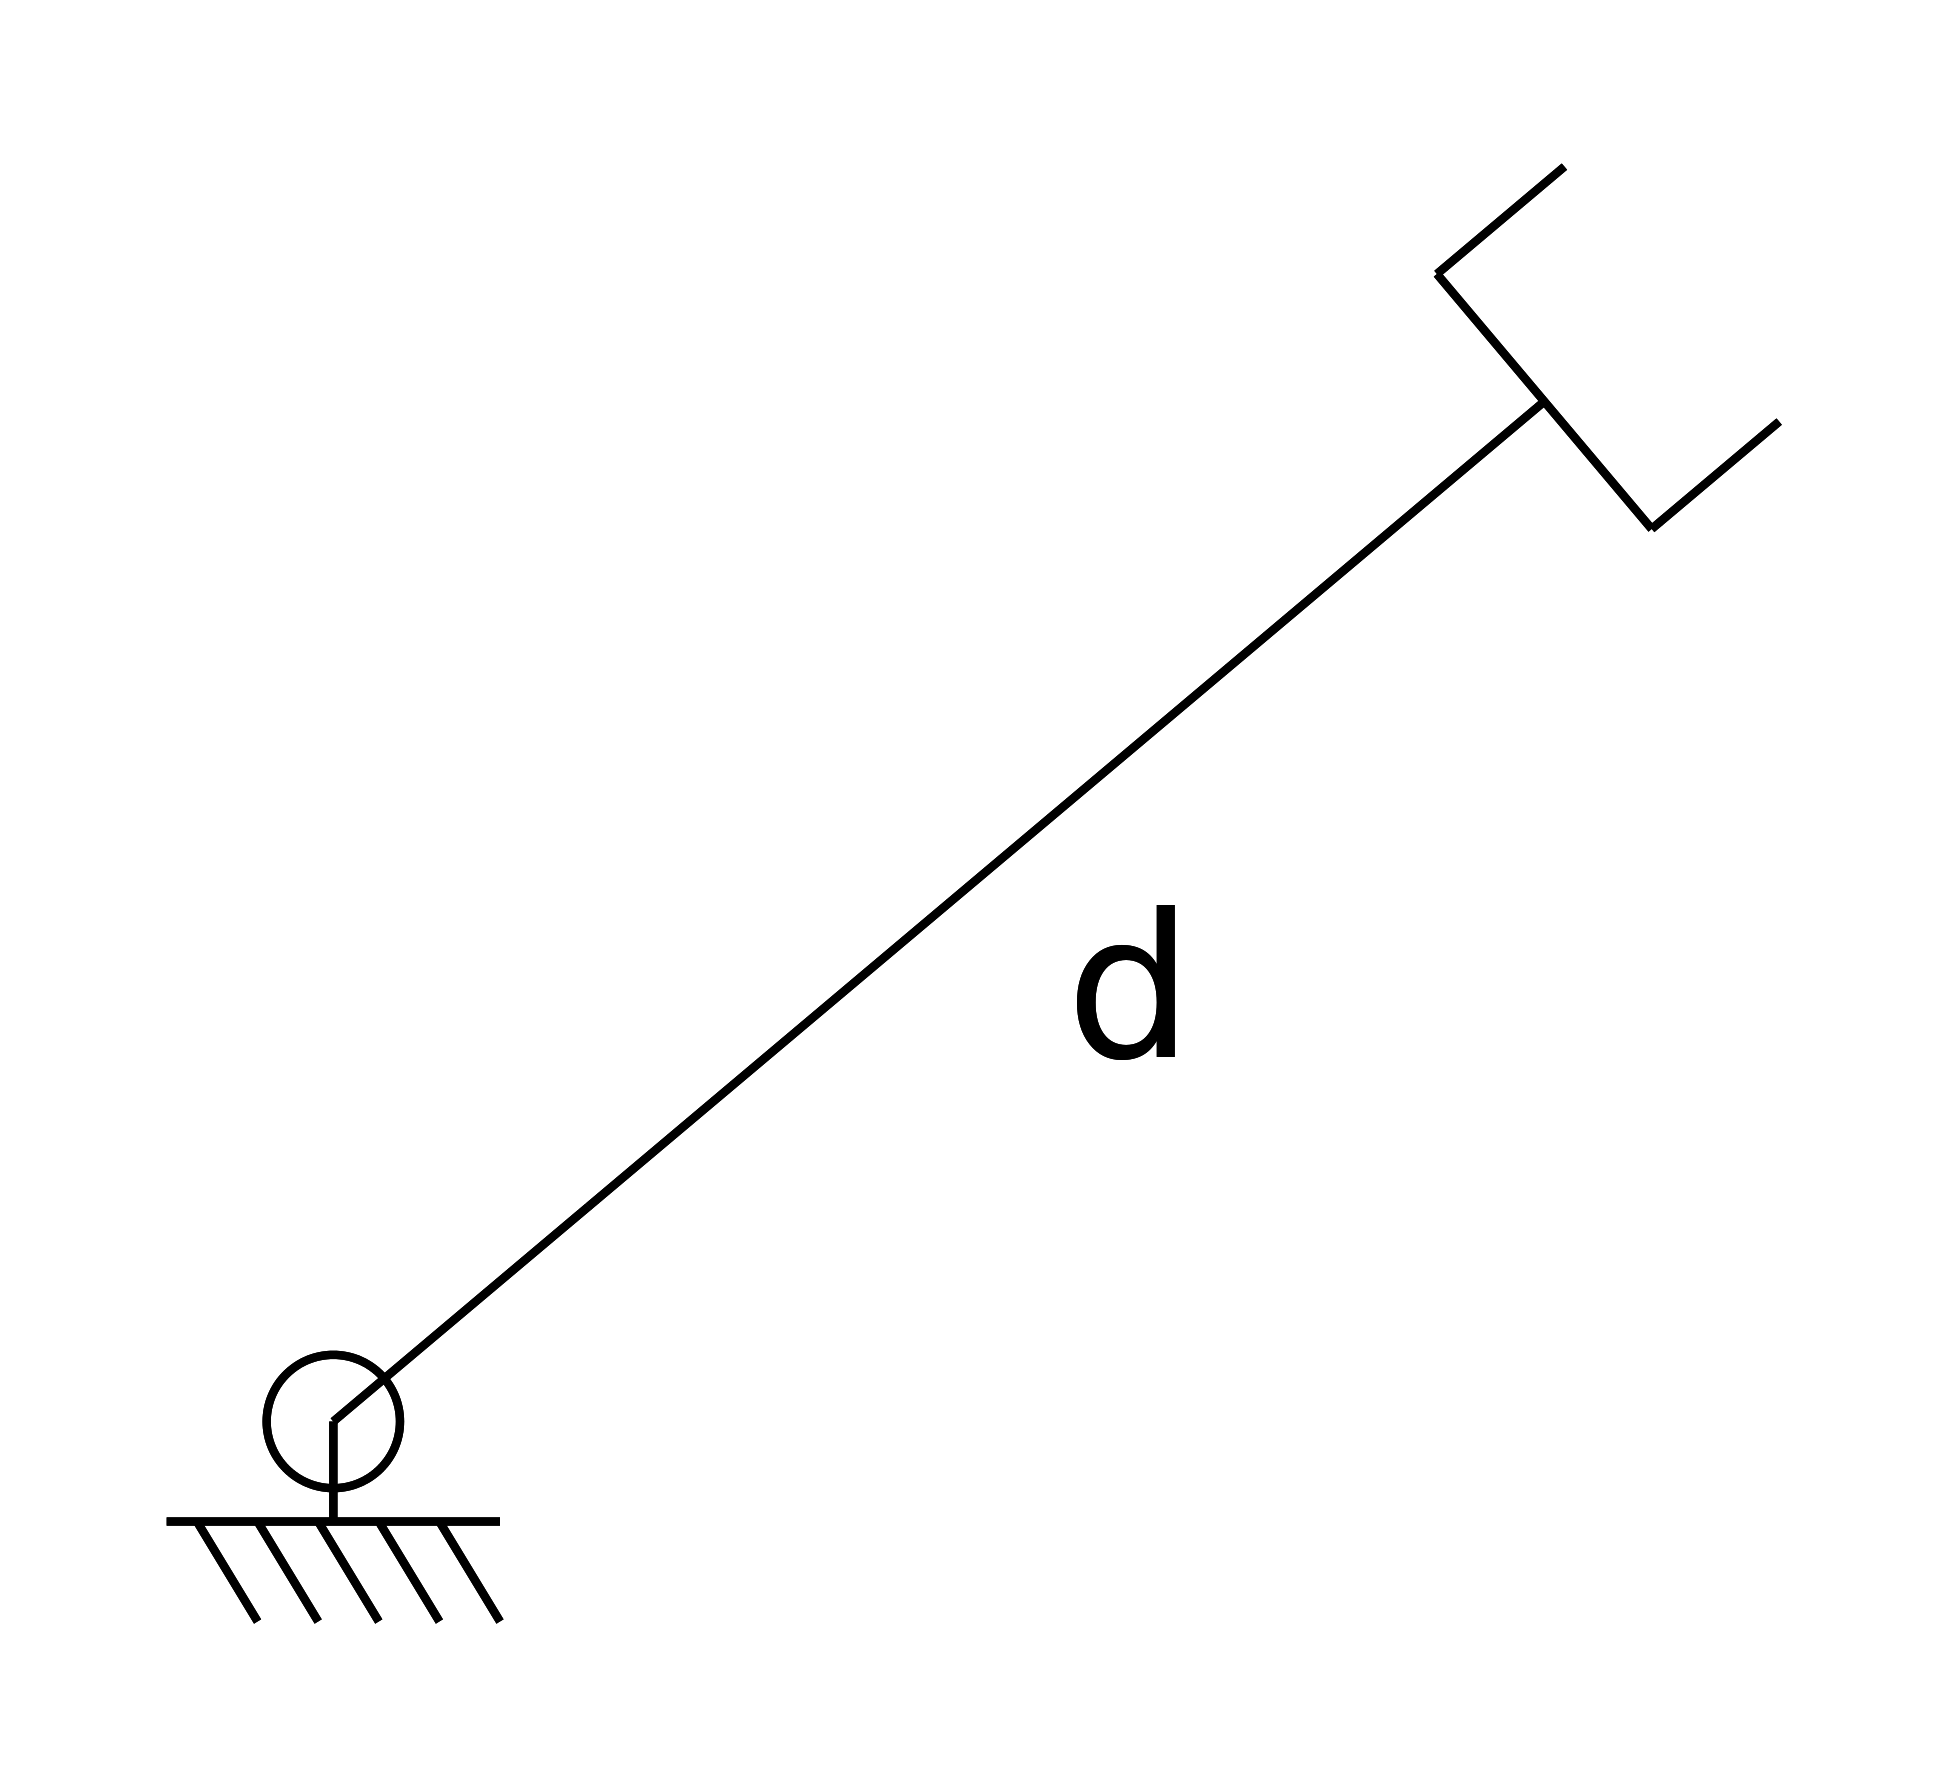
\includegraphics[scale=0.08]{generated_figures/bg_r_robot.png}
\end{center}

We wish to find the end effector position.  First, we can find it analytically
by noting that $x = d \cos(\th)$ and $y = d \sin(\th)$.  In vector form,
\smcolvec{x\\y} = \smcolvec{d \cos(\th)\\d\sin(\th)}.  While finding the forward
kinematics algebraically will always work, it definitely gets more error prone
with larger systems, and when composing multiple arms.  The way around this is using
homogeneous transforms.

We define one frame at the base, the base frame, usually labeled \vec{0}.
Let \frame{1} be another frame at the base of the link, but rotated by \th.
Finally, let \frame{2} be based at the end of the link, such that
$\transform{p}{e}{2} = \smcolvec{0\\0}$ in that frame is the end-effector position.

% [Drawing of said frames.]
\begin{center}
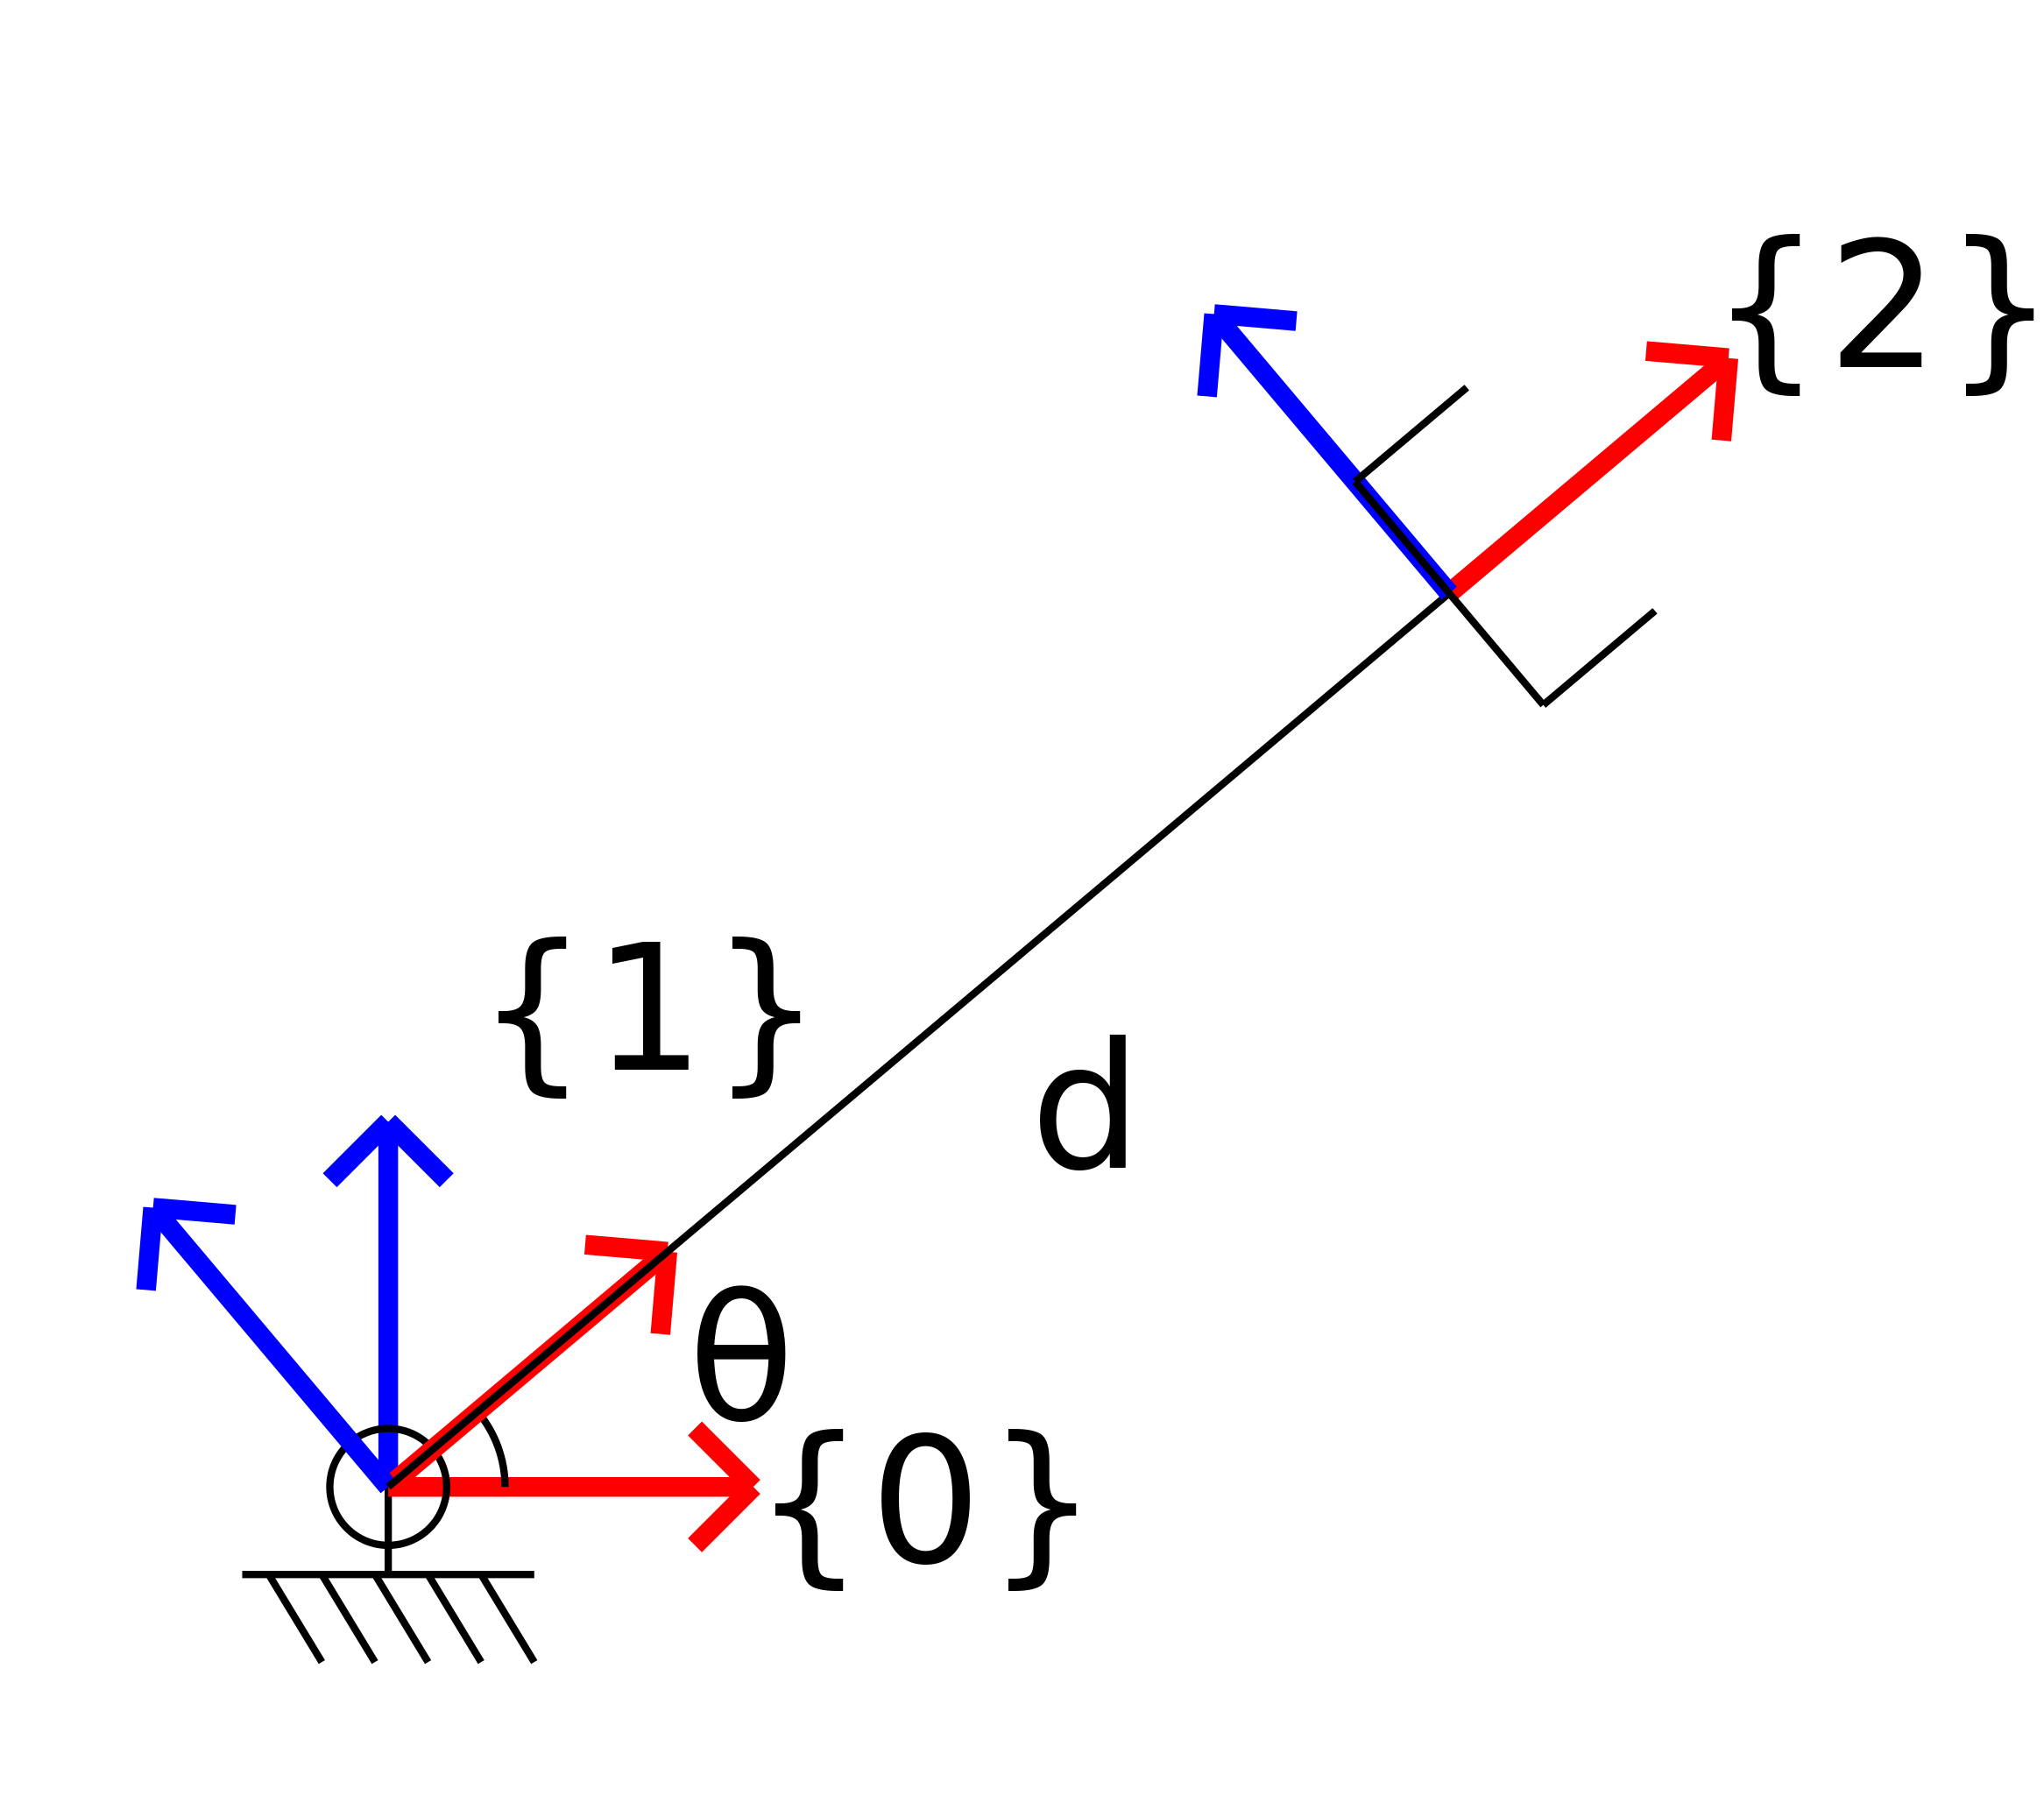
\includegraphics[scale=0.08]{generated_figures/bg_r_robot_frames.png}
\end{center}

Note that:

\begin{itemize}
    \item \H{1}{0} = \smcolvec{\mat{R_{\th}}&\vec{0}\\\trans{\vec{0}}&1} =
        \smcolvec{\cos(\th)&-\sin(\th)&0\\\sin(\th)&\cos(\th)&0\\0&0&1}
    \item \H{2}{1} = \smcolvec{1&0&d\\0&1&0\\0&0&1}
\end{itemize}

Therefore, \H{2}{0} = \H{1}{0}\H{2}{1} = \smcolvec{\cos(\th)&-\sin(\th)&d
\cos(\th)\\\sin(\th)&\cos(\th)&d\sin(\th)\\0&0&1}. Lastly, we can see that
$\H{2}{0} \transform{p}{e}{2} = \H{2}{0} \smcolvec{0\\0\\1} = \smcolvec{d \cos(\th)\\d \sin(\th)}$, which matches our analytical solution.

\end{document}
